\documentclass[12pt,a4paper,oneside, openright]{book}
\usepackage[ left=3cm,right=2.5cm,top=2.5cm,bottom=2.5cm]{geometry}

\usepackage[italian]{babel}
\usepackage{setspace}
\usepackage{graphicx}
\usepackage{hyperref}
\usepackage{fancyhdr}
\usepackage{subcaption}
\usepackage{csvsimple}
\usepackage{amsmath}
\usepackage{amssymb}
\usepackage{float}



\graphicspath{ {immagini/} }
\doublespacing
\fancyhf{}
\newcommand{\R}{\mathbb{R}}



\begin{document}
	\pagestyle{plain}
	\begin{titlepage}
\onehalfspacing


 \ \\ \ \\
\begin{figure}[htbp]
\begin{center}

\includegraphics[angle=0, height=3.7cm]{logo.jpg}
\end{center}
\end{figure}


\begin{center}
\begin{large}
\textbf{UNIVERSITÀ DI PISA}
\end{large}

\textsl{Dipartimento di informatica}

\begin{normalsize}
\textsl{Corso di Laurea in Informatica}
\\
\end{normalsize}
\vspace{2cm}
	TESI DI LAUREA \\

\begin{Large}
	\textbf{Implementazione e valutazione di un modello probabilistico di data coverage per scenari di Mobile CrowdSensing} \\
\end{Large}


\ \\ \ \\
\end{center}

\begin{normalsize}
\begin{flushleft}
\textit{Relatori}  \hspace{238pt} \textit{Candidato}
\\ \vspace{5pt} Prof. Stefano Chessa \hspace{6cm} Tommaso Colella
 \\ \vspace{5pt} Dr. Michele Girolami
\end{flushleft}

\end{normalsize}

\vspace{2cm}
\begin{center}
\small{Anno Accademico 2019/2020}
\end{center}

\end{titlepage}

\clearpage\null\thispagestyle{empty}\clearpage     %inserisce una pagina bianca senza numerarla
	\frontmatter
	\null\vspace{\stretch{1}}
\begin{flushright}
\emph{A mia nonna Paola}
\end{flushright}
\vspace{\stretch{2}}\null
\newpage
	
\begin{singlespace}
	\begin{center}
		\textsc{riassunto}
	\end{center}

I sistemi di Mobile CrowdSensing permettono di creare data set utilizzando le rilevazioni prodotte dai sensori presenti su dispositivi personali, indossabili, etc.
Uno degli aspetti di interesse per tale paradigma è misurare la qualità, ovvero la rappresentatività, dei dati che possono essere acquisiti. Tale problema prende il nome di Data Coverage.
	
In questa tesi ci prefiggiamo di implementare e applicare un modello probabilistico di Data Coverage in un contesto urbano basandoci sullo stato dell'arte.
Applichiamo il modello al dataset Microsoft Geolife, dopo averlo opportunamente arricchito per ovviare alla mancanza di dati.
Mettiamo inoltre a confronto il data set ottenuto con l'originale per valutare la bontà dell'arricchimento effettuato.
Nel seguito, studiamo la Data Coverage calcolata dal modello per una serie di scenari di Mobile Crowdsensing nell'area metropolitana di Pechino.
Gli scenari selezionati si legano a specifiche problematiche proprie delle smart cities, siano esse esigenze di monitoraggio ambientale, controllo dei flussi di traffico o di raccolta dati da punti di interesse dislocati nella metropoli.
Per ciascuno scenario mostriamo i risultati del nostro esperimento per mezzo di opportune mappe di calore.
	
Tramite questo studio otteniamo alcuni data set di Coverage per ciascuno scenario considerato, adatti a pianificare future campagne di raccolta dati di vario genere.
	
\end{singlespace}

	
	\mainmatter
	\hypersetup{linkcolor=black}
\tableofcontents
\listoffigures
	\chapter*{Introduzione}
\addcontentsline{toc}{chapter}{Introduzione}

La diffusione massiccia di dispositivi indossabili, e la loro sempre maggiore potenza di calcolo, hanno dato origine ad un recente paradigma computazionale denominato Mobile Crowdsensing (o MCS). Tale paradigma permette di raccogliere dati sull'ambiente che ci circonda e di analizzarli. Le applicazioni del MCS sono molteplici. Nel caso delle Smart Cities, il MCS può contribuire a migliorarne la vivibilità, la sicurezza e la interconnettività, sfruttando le capacità sensoriali e di calcolo dei dispositivi.

Grazie al Crowdsensing è possibile creare data set utilizzando rilevazioni ottenute dai dispositivi personali degli utenti. Tali dataset possono poi essere inviati ad un server remoto che svolga analisi approfondite su di essi e restituisca delle metriche utili.
Molti gruppi di ricerca (accademici e industriali) si sono interessati al Crowdsensing e hanno prodotto negli anni una moltitudine di articoli che esplorano i vari aspetti di questa metodologia di raccolta dati. Dedicheremo la Sezione 1.1 del Capitolo 1 a presentare il Crowdsensing con la dovuta profondità, mostrando i principali ambiti in cui è stato impiegato e presentando gli articoli fondamentali che ne hanno determinato l'origine.
Successivamente, nella Sezione 1.2, daremo una prima descrizione dei data set di mobilità urbana, sottolineandone l'utilità nell'ambito del Crowdsensing e presentando i più noti tra di essi. 


Uno dei problemi strettamente legati al MCS è quello di misurare la copertura dei dati che possiamo aspettarci per una determinata campagna di raccolta.
Per probabilità di copertura, o Data Coverage, intendiamo la probabilità che gli utenti che partecipano volontariamente alla nostra campagna di Crowdsensing si avvicinino alle locazioni di interesse per la campagna di MCS in modo da poter acquisire i dati.
Nel seguito ci riferiremo ad essa chiamandola alternativamente "Data Coverage", "probabilità di copertura", o anche solo "Coverage", quando il significato risulti chiaro dal contesto.

 Per modellare la probabilità di copertura utilizzeremo una funzione di densità di probabilità che andremo a descrivere nel Capitolo 2, in cui approfondiremo maggiormente il concetto di Data Coverage.
  La Figura \ref{fig:coverage_examples} mostra una rappresentazione grafica della Data Coverage ottenuta per mezzo di una meshgrid.
  
 \begin{figure}[h!]
 	\centering
 	\begin{subfigure}[b]{0.5\linewidth}
 		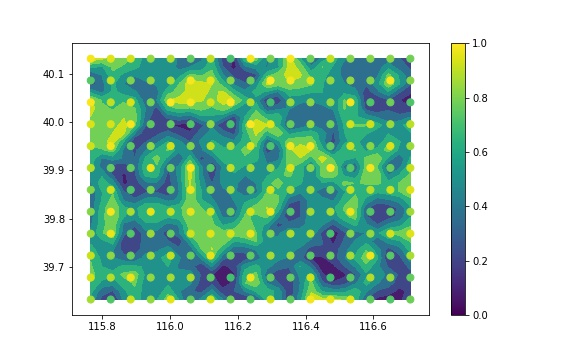
\includegraphics[width=\linewidth]{well_covered_meshgrid.jpg}
 		\caption{Buona Data Coverage}
 	\end{subfigure}\hfill
 	\begin{subfigure}[b]{0.5\linewidth}
 		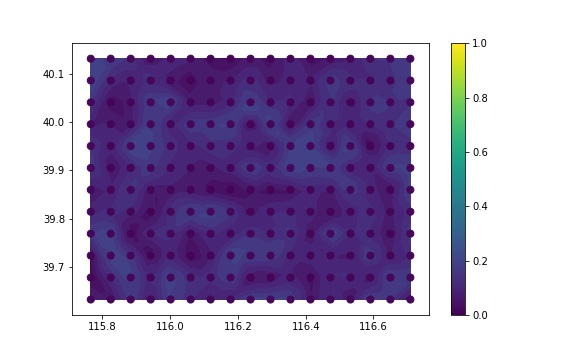
\includegraphics[width=\linewidth]{badly_covered_meshgrid.jpg}
 		\caption{Cattiva Data Coverage}
 	\end{subfigure}\hfill
 	\caption[Esempio di Data Coverage]{Esempi di Data Coverage su una griglia di locazioni}
 	\label{fig:coverage_examples}
 \end{figure}

\ \\ \\
 
 
La presente tesi ha come obiettivo quello di implementare una misura di copertura utilizzando un modello probabilistico che tenga conto della mobilità degli utenti che partecipano alla campagna.
Tale modello deve essere facilmente utilizzabile in scenari di raccolta dati differenti.
Al fine di misurare la Data Coverage, è stato analizzato ed esteso il data set GeoLife \cite{zheng1,zheng2,zheng3}.
Il data set offre tracciati GPS raccolti su base volontaria in un periodo temporale molto ampio; questo porta a problematiche di vario tipo: la campionatura dei punti GPS non è regolare e vi sono intere settimane nel nostro data set che mancano di dati significativi per la scarsa partecipazione degli utenti; nel corso della tesi tale data set è stato esteso, generando in questo modo Augmented Geolife, di cui daremo una descrizione approfondita nel Capitolo 3, dopo aver parlato del data set originale.

\section*{Obiettivi della Tesi}


La presente tesi ha due obiettivi principali:
\begin{enumerate}
	\item Analizzare ed estendere un data set di mobilità
	\item Sviluppare un modello di Data Coverage
\end{enumerate}

In merito al primo obiettivo la tesi ha permesso di ottenere un data set aumentato per la città di Pechino, contenente una quantità di dati sufficienti al prosieguo delle analisi.
In merito al secondo obiettivo, lo sviluppo del modello di Data Coverage e la sua applicazione a differenti scenari applicativi, ci ha permesso di ottenere delle mappe di probabilità di copertura dell'area oggetto della campagna di Crowdsensing.
Tali mappe ci possono aiutare a pianificare future campagne di acquisizione dati, e sono sufficientemente chiare da permettere una identificazione rapida ed efficace delle zone che risultano essere scoperte, zone per cui dovremo probabilmente prevedere campagne di raccolta ad hoc.

La misurazione della Data Coverage è di estrema importanza per una serie di motivi: oltre a permetterci di valutare in modo quantitativo l'efficacia di una campagna di crowdsensing, ci fornisce anche un modo per pianificare ulteriori meccanismi di raccolta dati che siano complementari al paradigma di MCS. Uno tra questi potrebbe essere l'utilizzo di droni da inviare su richiesta nelle zone scarsamente coperte, in modo da migliorarne il parametro di coverage.
Un altro dei vantaggi della misurazione della Data Coverage è quello di dare informazioni su quali siano le aree urbane scarsamente popolate o trafficate. Grazie alla visualizzazione grafica dei data set di probabilità ottenuti per i vari scenari, è possibile comprendere facilmente tali risultati sperimentali.

\section*{Metodologia e Risultati}

\subsection*{Metodologia usata}

Per raggiungere i nostri scopi ci siamo avvalsi di una serie di librerie software all'avanguardia nel campo della mobilità, dell'analisi dati e della visualizzazione di questi ultimi. Nella Sezione 1.3 presenteremo le librerie che ci hanno aiutati maggiormente nella nostra analisi. Tra di esse è sicuramente importante ricordare scikit-mobility \cite{pappalardo2019scikitmobility}, strumento grazie al quale abbiamo elaborato con semplicità ed efficacia i dati spaziali.
Nel corso della tesi abbiamo progettato e sviluppato processi simulativi per arricchire il data set Geolife con ulteriori traiettorie.
L'utilizzo di strumenti di visual analytics ci ha infine permesso di rappresentare le proprietà dei dati spaziali che abbiamo analizzato.

\subsection*{Risultati ottenuti}

Lo studio ci ha condotti allo sviluppo di opportune analitiche per misurare le proprietà del data set GeoLife, tra di esse citiamo il numero di utenti attivi in un determinato periodo temporale, i punti di partenza e di arrivo delle traiettorie degli utenti, i flussi di spostamenti sulla città di Pechino.

Abbiamo inoltre sviluppato un simulatore di tracce che, per mezzo di interpolazioni e calcoli di distanze, permette di generare serie temporali di traiettorie sintetiche con una certa precisione basandoci su punti di partenza e di arrivo.

Altro importante risultato ottenuto è l'implementazione di un modello di Data Coverage basato sulla probabilità di detour degli utenti. 

I risultati della applicazione del modello ai vari scenari sono presentati nel Capitolo 4 assieme a delle mappe di calore che ne riassumono graficamente il significato. La rappresentazione grafica ci mostra intere zone completamente scoperte per ciascuno dei tre scenari che abbiamo preso in esame, e ci invita a indagare soluzioni future atte a migliorare la Data Coverage nella zona che abbiamo preso come riferimento.
Di tali sviluppi futuri facciamo menzione nel Capitolo 5.

	\input{cap1}
	\input{cap2}
	\input{cap3}
	\chapter{Sperimentazioni e analisi dei risultati}
In questo capitolo descriviamo la sperimentazione effettuata grazie al modello di Data Coverage e alle traiettorie di Augmented Geolife.
Daremo una descrizione per ciascuno degli scenari applicativi del modello, e successivamente presenteremo i risultati sperimentali, fornendone anche una opportuna visualizzazione grafica. Dapprima parleremo del monitoraggio ambientale, spostandoci poi sul monitoraggio dei flussi di traffico e trattando infine il sensing basato su punti di interesse.

Nell'ultima sezione del capitolo, cercheremo di interpretare i risultati ottenuti per ciascuno scenario.


\section{Tre scenari applicativi}
In questa tesi abbiamo preso in esame tre diversi scenari applicativi. Ciascuno di essi rappresenta un diverso ambito di applicazione della Data Coverage e, più in generale, del paradigma del Mobile Crowdsensing.
Con scenario applicativo intendiamo un diverso posizionamento delle locazioni di raccolta dati, guidato dall'obiettivo che vogliamo raggiungere. Tali differenze nei posizionamenti sono state considerate principalmente per mostrare l'efficienza del modello di copertura in diversi contesti di raccolta dati.
 
Nel seguito del capitolo evidenzieremo le peculiarità di ciascuno scenario, fornendo contestualmente i risultati dell'applicazione del modello di Data Coverage.

Il procedimento sperimentale seguito per ciascuno scenario è il seguente:
\begin{enumerate}
	\item Dato uno scenario, ne abbiamo identificato le locazioni tramite generazione o estrazione dal database di OpenStreetMap.
	\item Abbiamo considerato tre diversi valori di $\lambda$ per modellare la probabilità che un utente sia disposto ad accettare un detour, come descritto nel Capitolo 2. 
	\item Applicando il modello alle locazioni dello scenario abbiamo ottenuto i valori di coverage per ciascuna di esse.
	\item Utilizzando grafici di vario tipo abbiamo dato una visualizzazione della Data Coverage.
\end{enumerate}

La Figura \ref{fig:pipeline} presenta la nostra pipeline di sperimentazione, utilizzata per ogni scenario.

Gli scenari presi in esame sono i seguenti:
\begin{itemize}
	\item Monitoraggio dei flussi di traffico
	\item Sensing basato su punti di interesse
	\item Monitoraggio ambientale basato su griglia
\end{itemize}


\begin{figure}[H]
	\centering 
	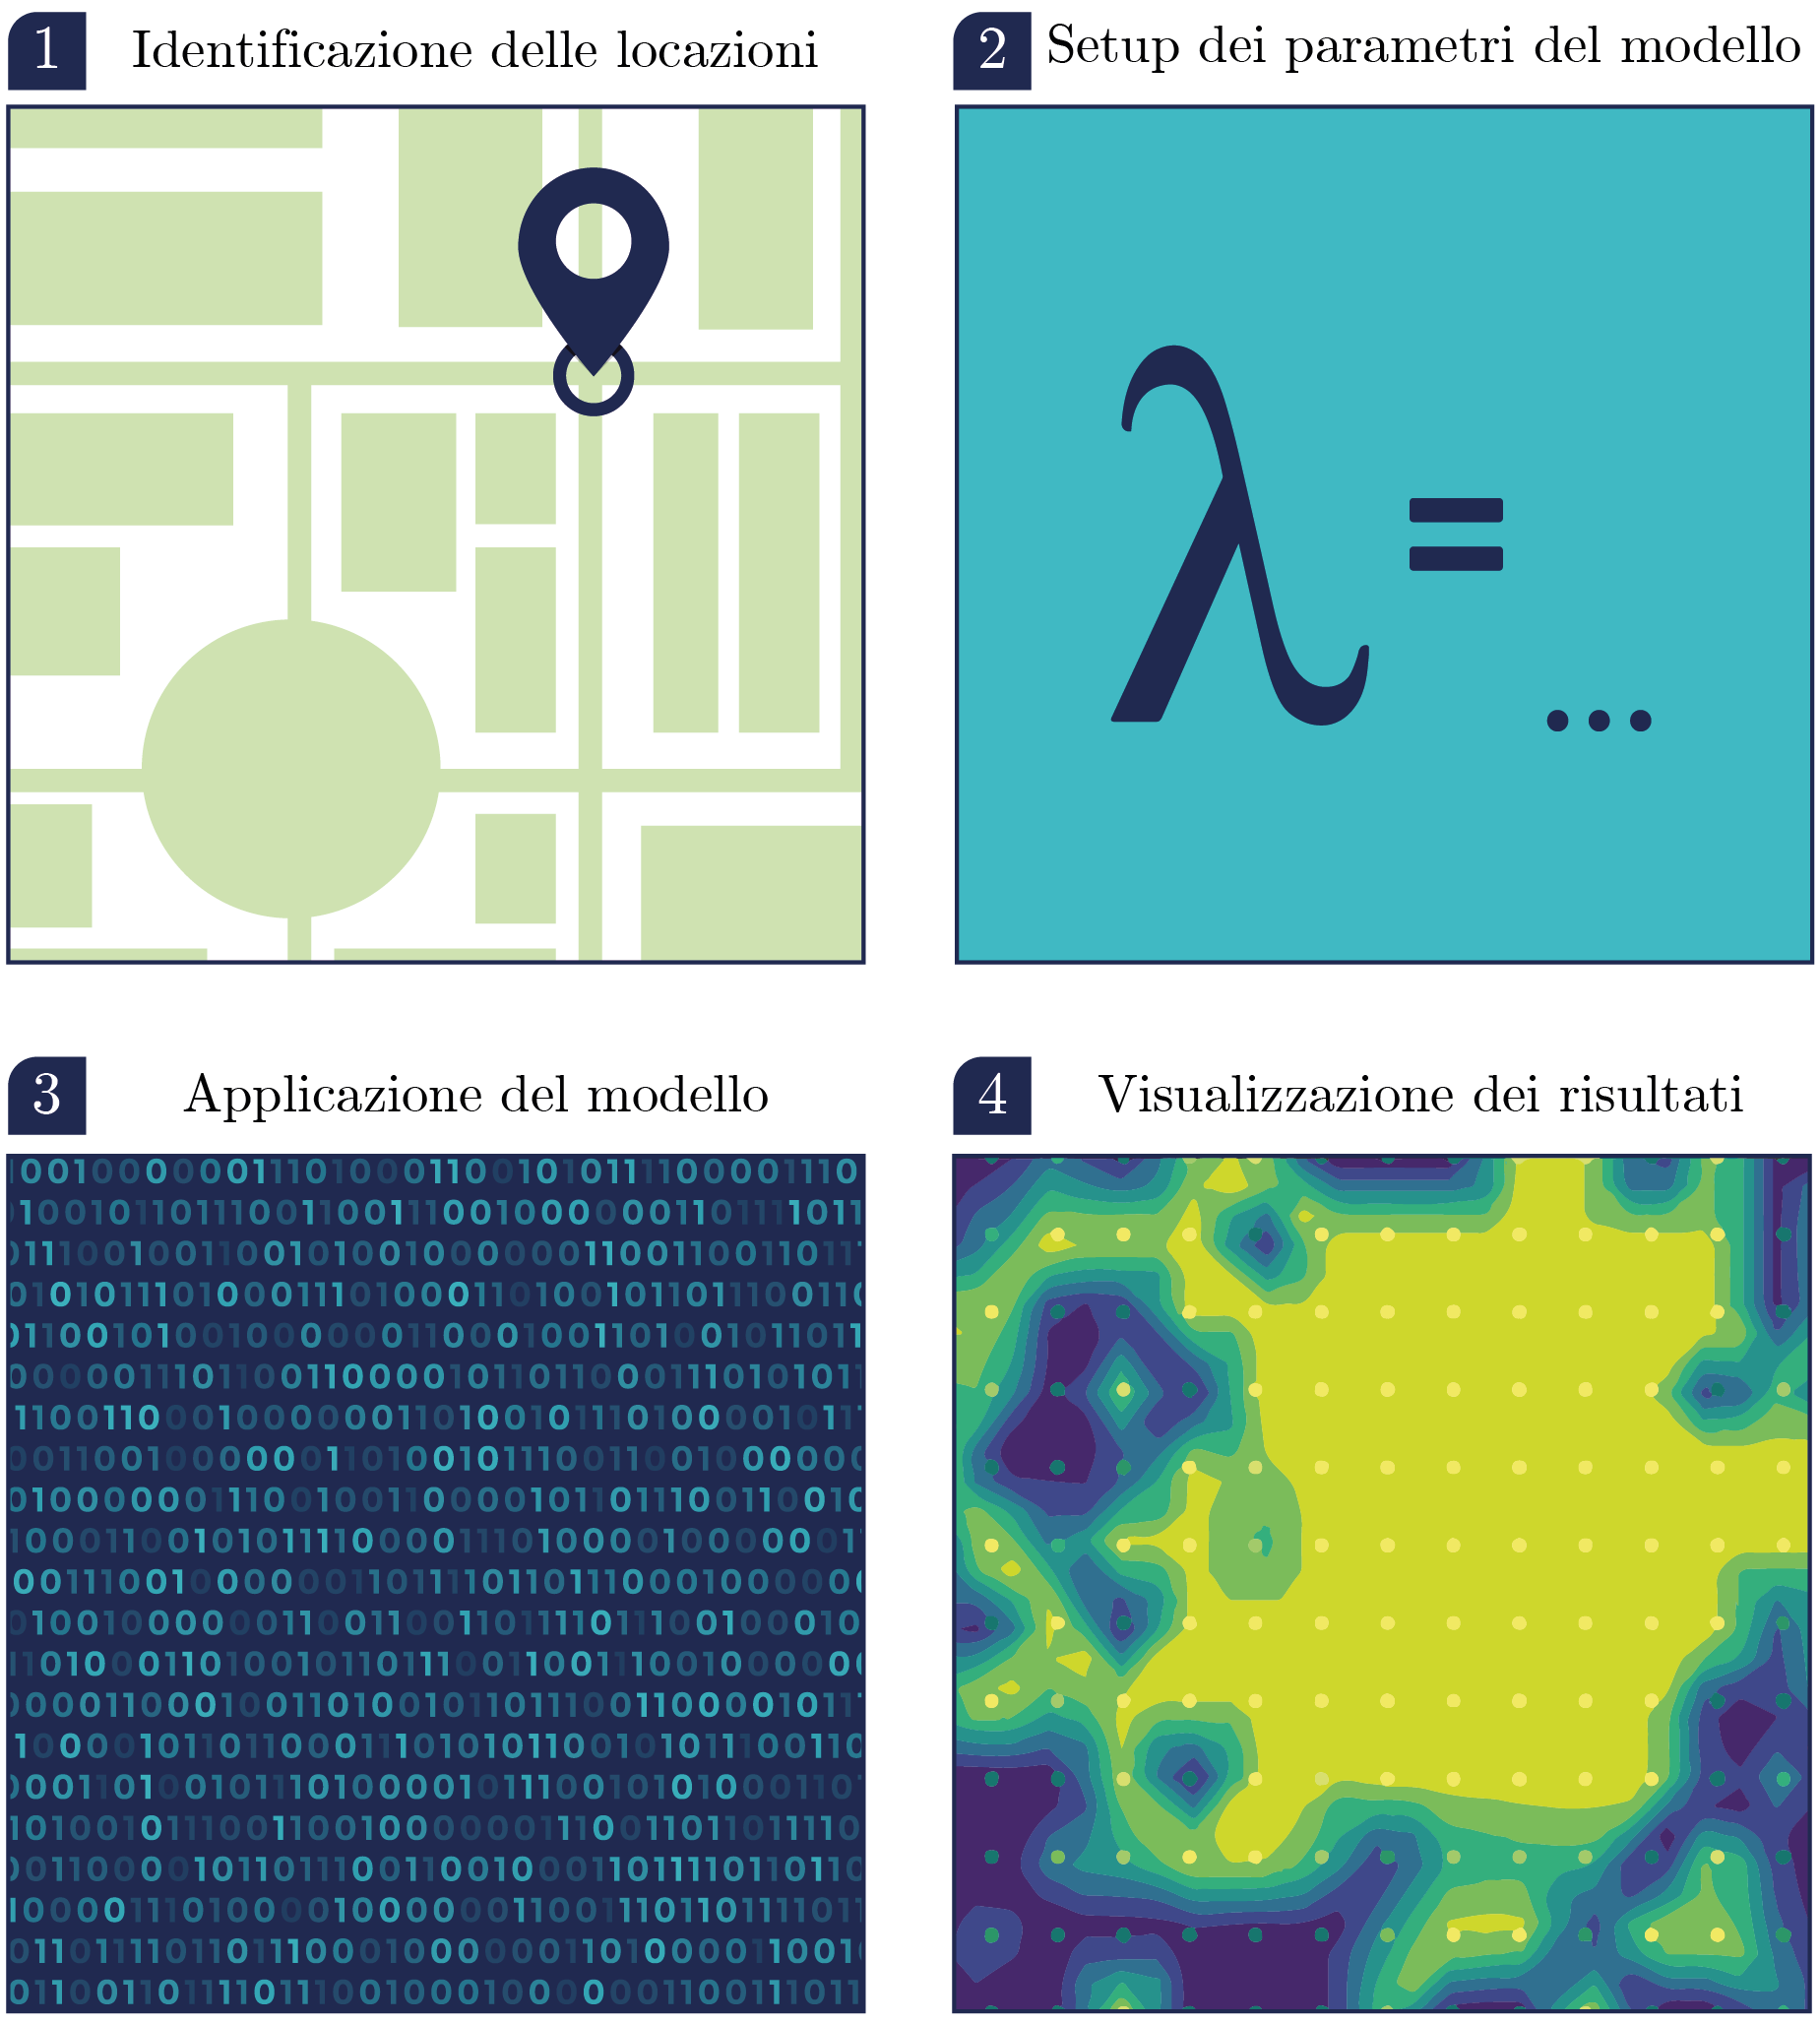
\includegraphics[width=\linewidth]{pipeline.png}
	\caption[Pipeline di sperimentazione]{L'immagine mostra la pipeline di sperimentazione utilizzata}
	\label{fig:pipeline}
\end{figure}


\section{Monitoraggio ambientale}
Lo scenario applicativo di monitoraggio ambientale si riferisce alla raccolta di dati utili al monitoraggio di parametri ambientali, come ad esempio: la temperatura, l'inquinamento acustico, la copertura e la qualità dei segnali wireless e molti altri. 

Per questa tipologia di MCS abbiamo preso in esame locazioni disposte a griglia ed equispaziate l'una dall'altra. Per fare ciò abbiamo opportunamente generato una griglia rettangolare più grande possibile che ricadesse all'interno dei confini geografici della macroarea di Pechino. L'idea è che i dati di tipo ambientale varino in modo molto meno netto rispetto a dati di altro tipo come possono essere quelli del traffico, per questa ragione la distanza tra le locazioni è nell'ordine dei chilometri, così da poter captare variazioni significative nei dati che devono essere raccolti. 

\subsection{Generazione della griglia}
Per la generazione della griglia ci siamo avvalsi di \textit{Shapely} \cite{shapely} e \textit{PiProj} \cite{pyproj}.
Dopo aver scelto gli estremi dell'area su cui generare la griglia, abbiamo impiegato queste librerie per ottenere le locazioni corrette. Grazie alla classe Point di Shapely e alle proiezioni fornite da PyProj, abbiamo iterativamente selezionato i punti della griglia prendendoli a distanza regolare sulla proiezione bidimensionale ottenuta. Successivamente li abbiamo riproiettati  a coordinate GCS sempre grazie a PyProj. 

Una volta ottenuta la griglia abbiamo provveduto a serializzarla per la successiva applicazione del modello.

Grazie a folium \cite{folium}, in Figura \ref{fig:grid}, possiamo visualizzare la griglia ottenuta.
Le locazioni sono identificate dai cerchi blu.
In sovraimpressione sono presenti alcune delle traiettorie di Augmented Geolife.

\begin{figure}[H]
	\centering 
	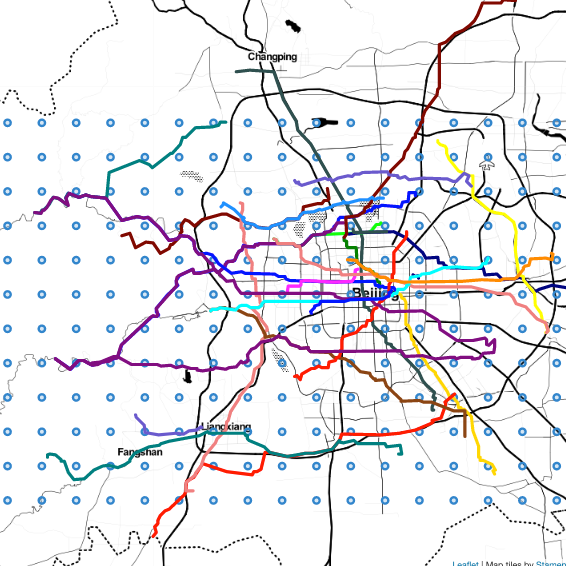
\includegraphics[width=\linewidth]{grid_folium.png}
	\caption[Griglia visualizzata con folium]{La griglia visualizzata per mezzo di folium}
	\label{fig:grid}
\end{figure}

\subsection{Risultati del modello di coverage}
Le Figure \ref{fig:grid_coverage1}, \ref{fig:grid_coverage2}, e \ref{fig:grid_coverage3}, mostrano i risultati ottenuti applicando il modello con differenti valori di lambda sulla griglia ottenuta. 
Dalle mappe di calore e meshgrid ottenute, si può notare come la Data Coverage vari al variare del paramentro $\lambda$, che modella la probabilità che gli utenti siano disposti ad accettare il detour verso le locazioni di raccolta dati.
Al crescere di $\lambda$ la Data Coverage migliora.
Le meshgrid e le mappe di calore sono state ottenute tramite interpolazione lineare sui risultati di Data Coverage ottenuti applicando il modello ad ogni singola locazione.

\begin{figure}[H]
	\centering
	\begin{subfigure}[b]{\linewidth}
		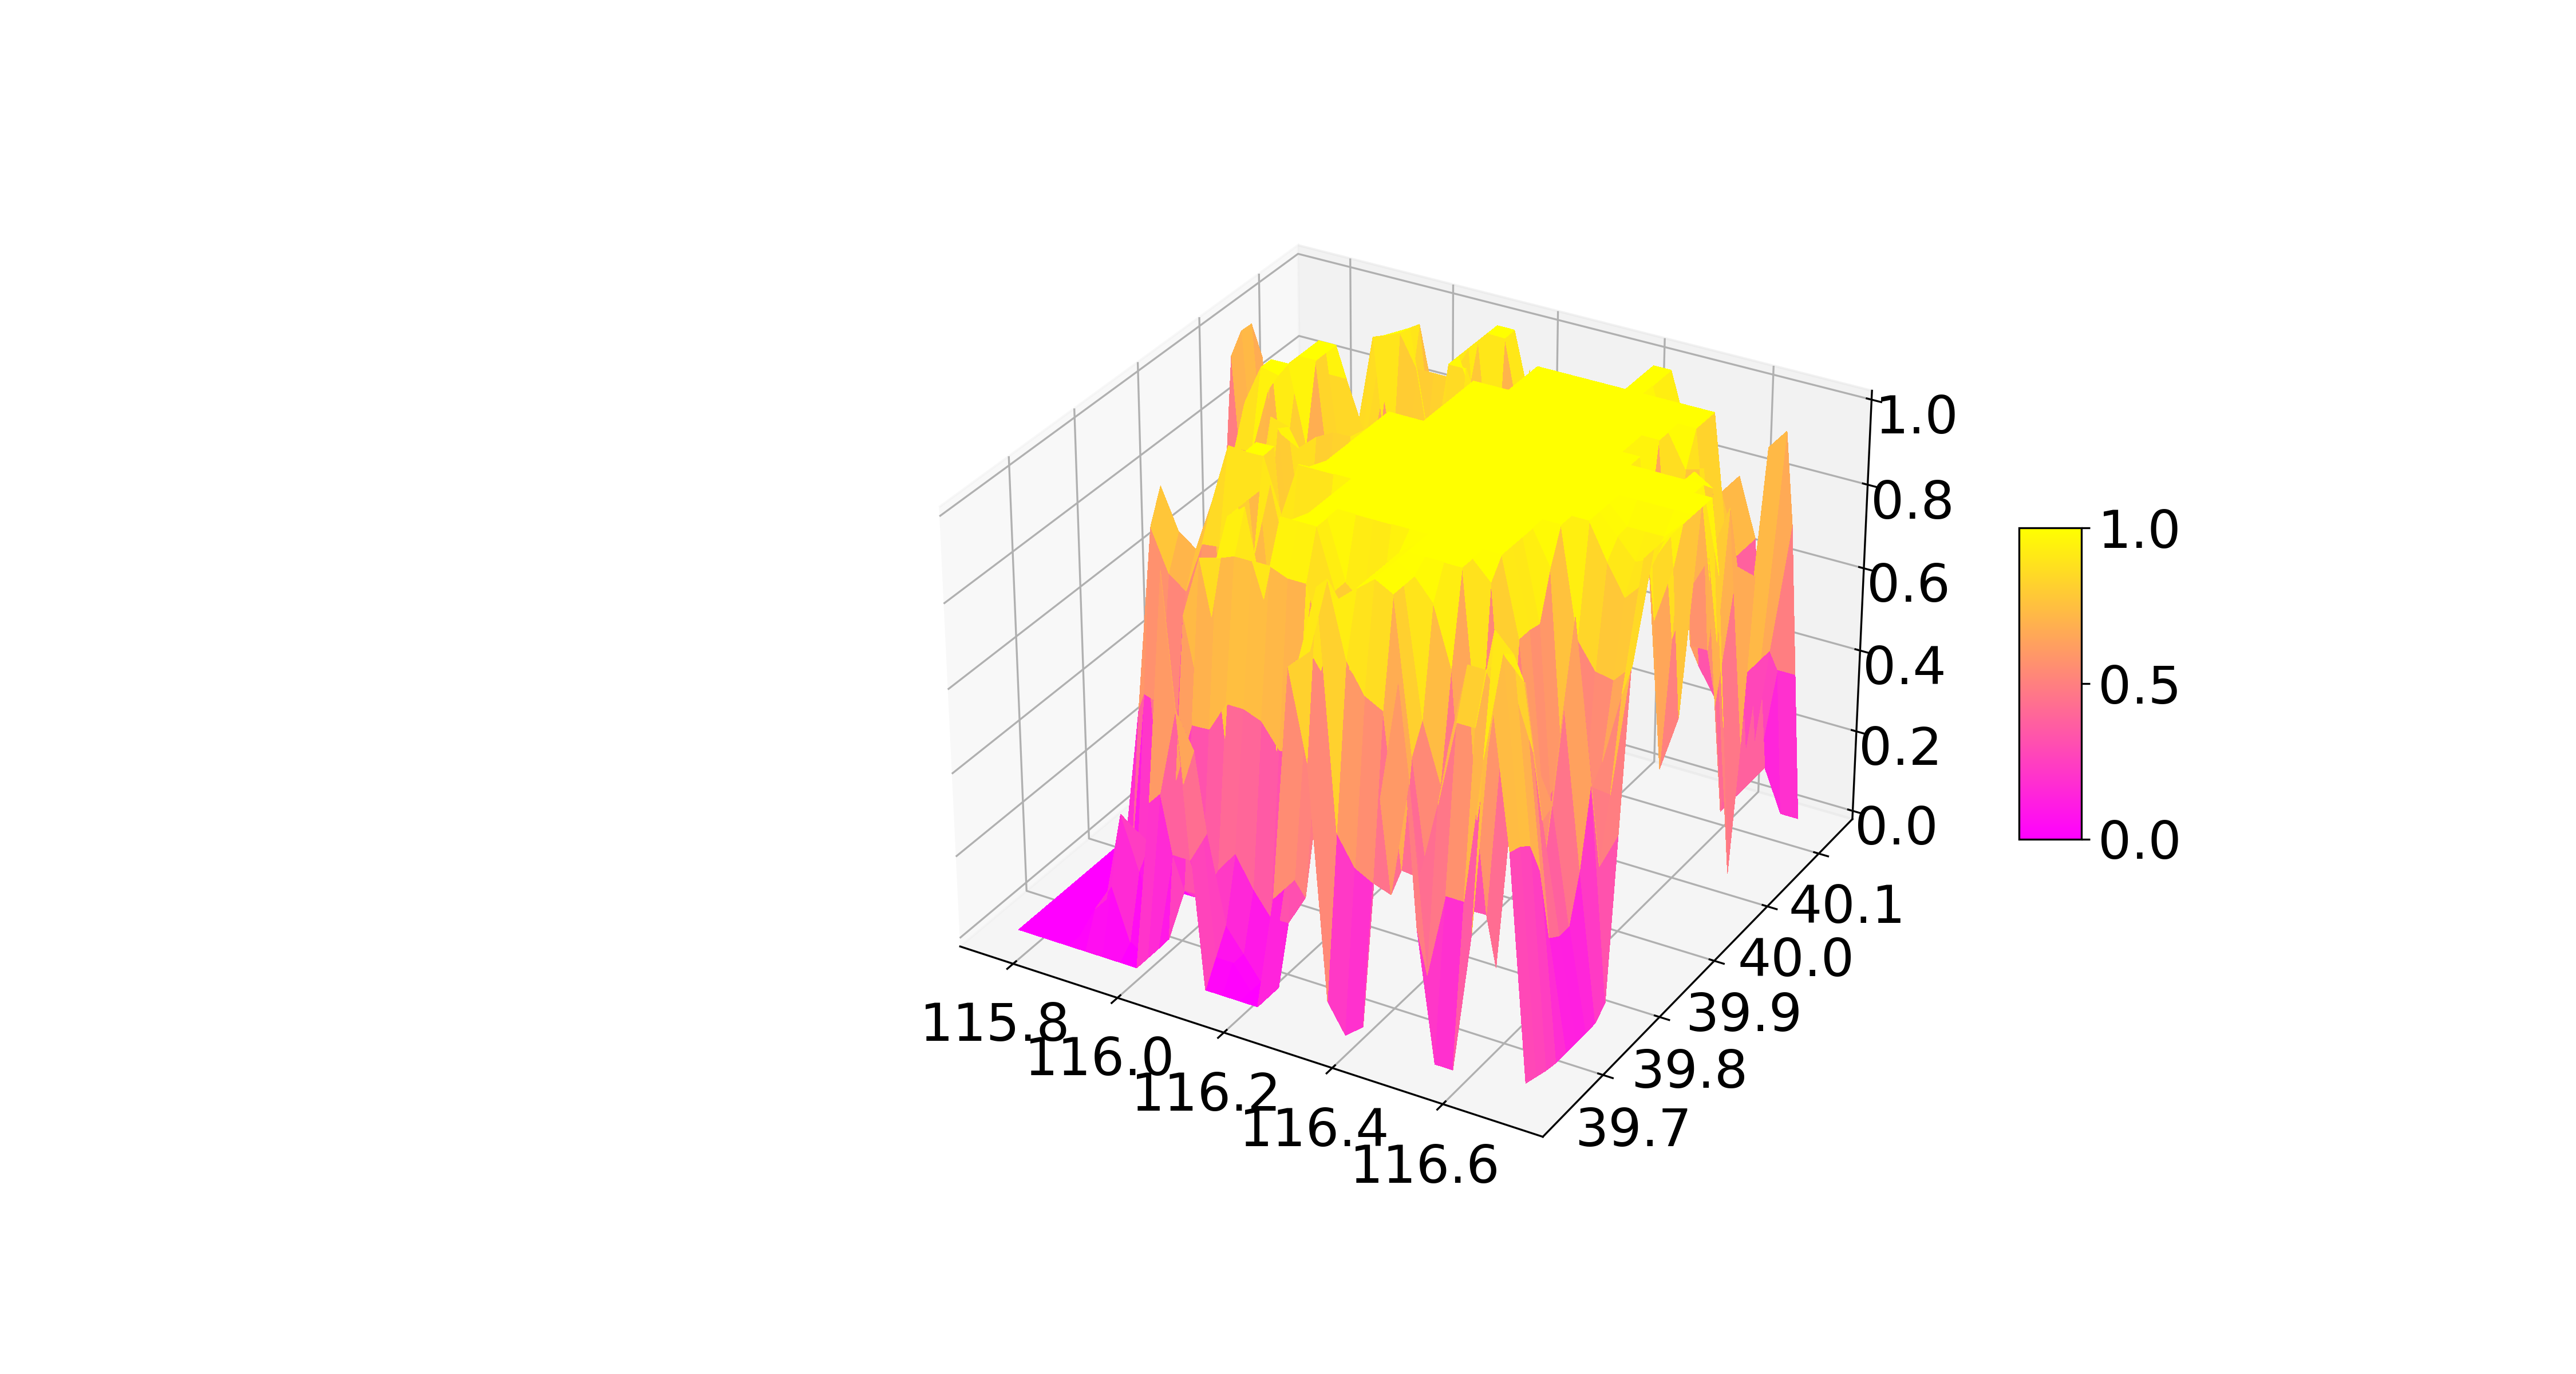
\includegraphics[width=\linewidth]{grid_coverages_0,01_lambda_3D_grid.png}
		\caption{Meshgrid ottenuta per $\lambda = 1/100$}
	\end{subfigure}
	\begin{subfigure}[b]{\linewidth}
		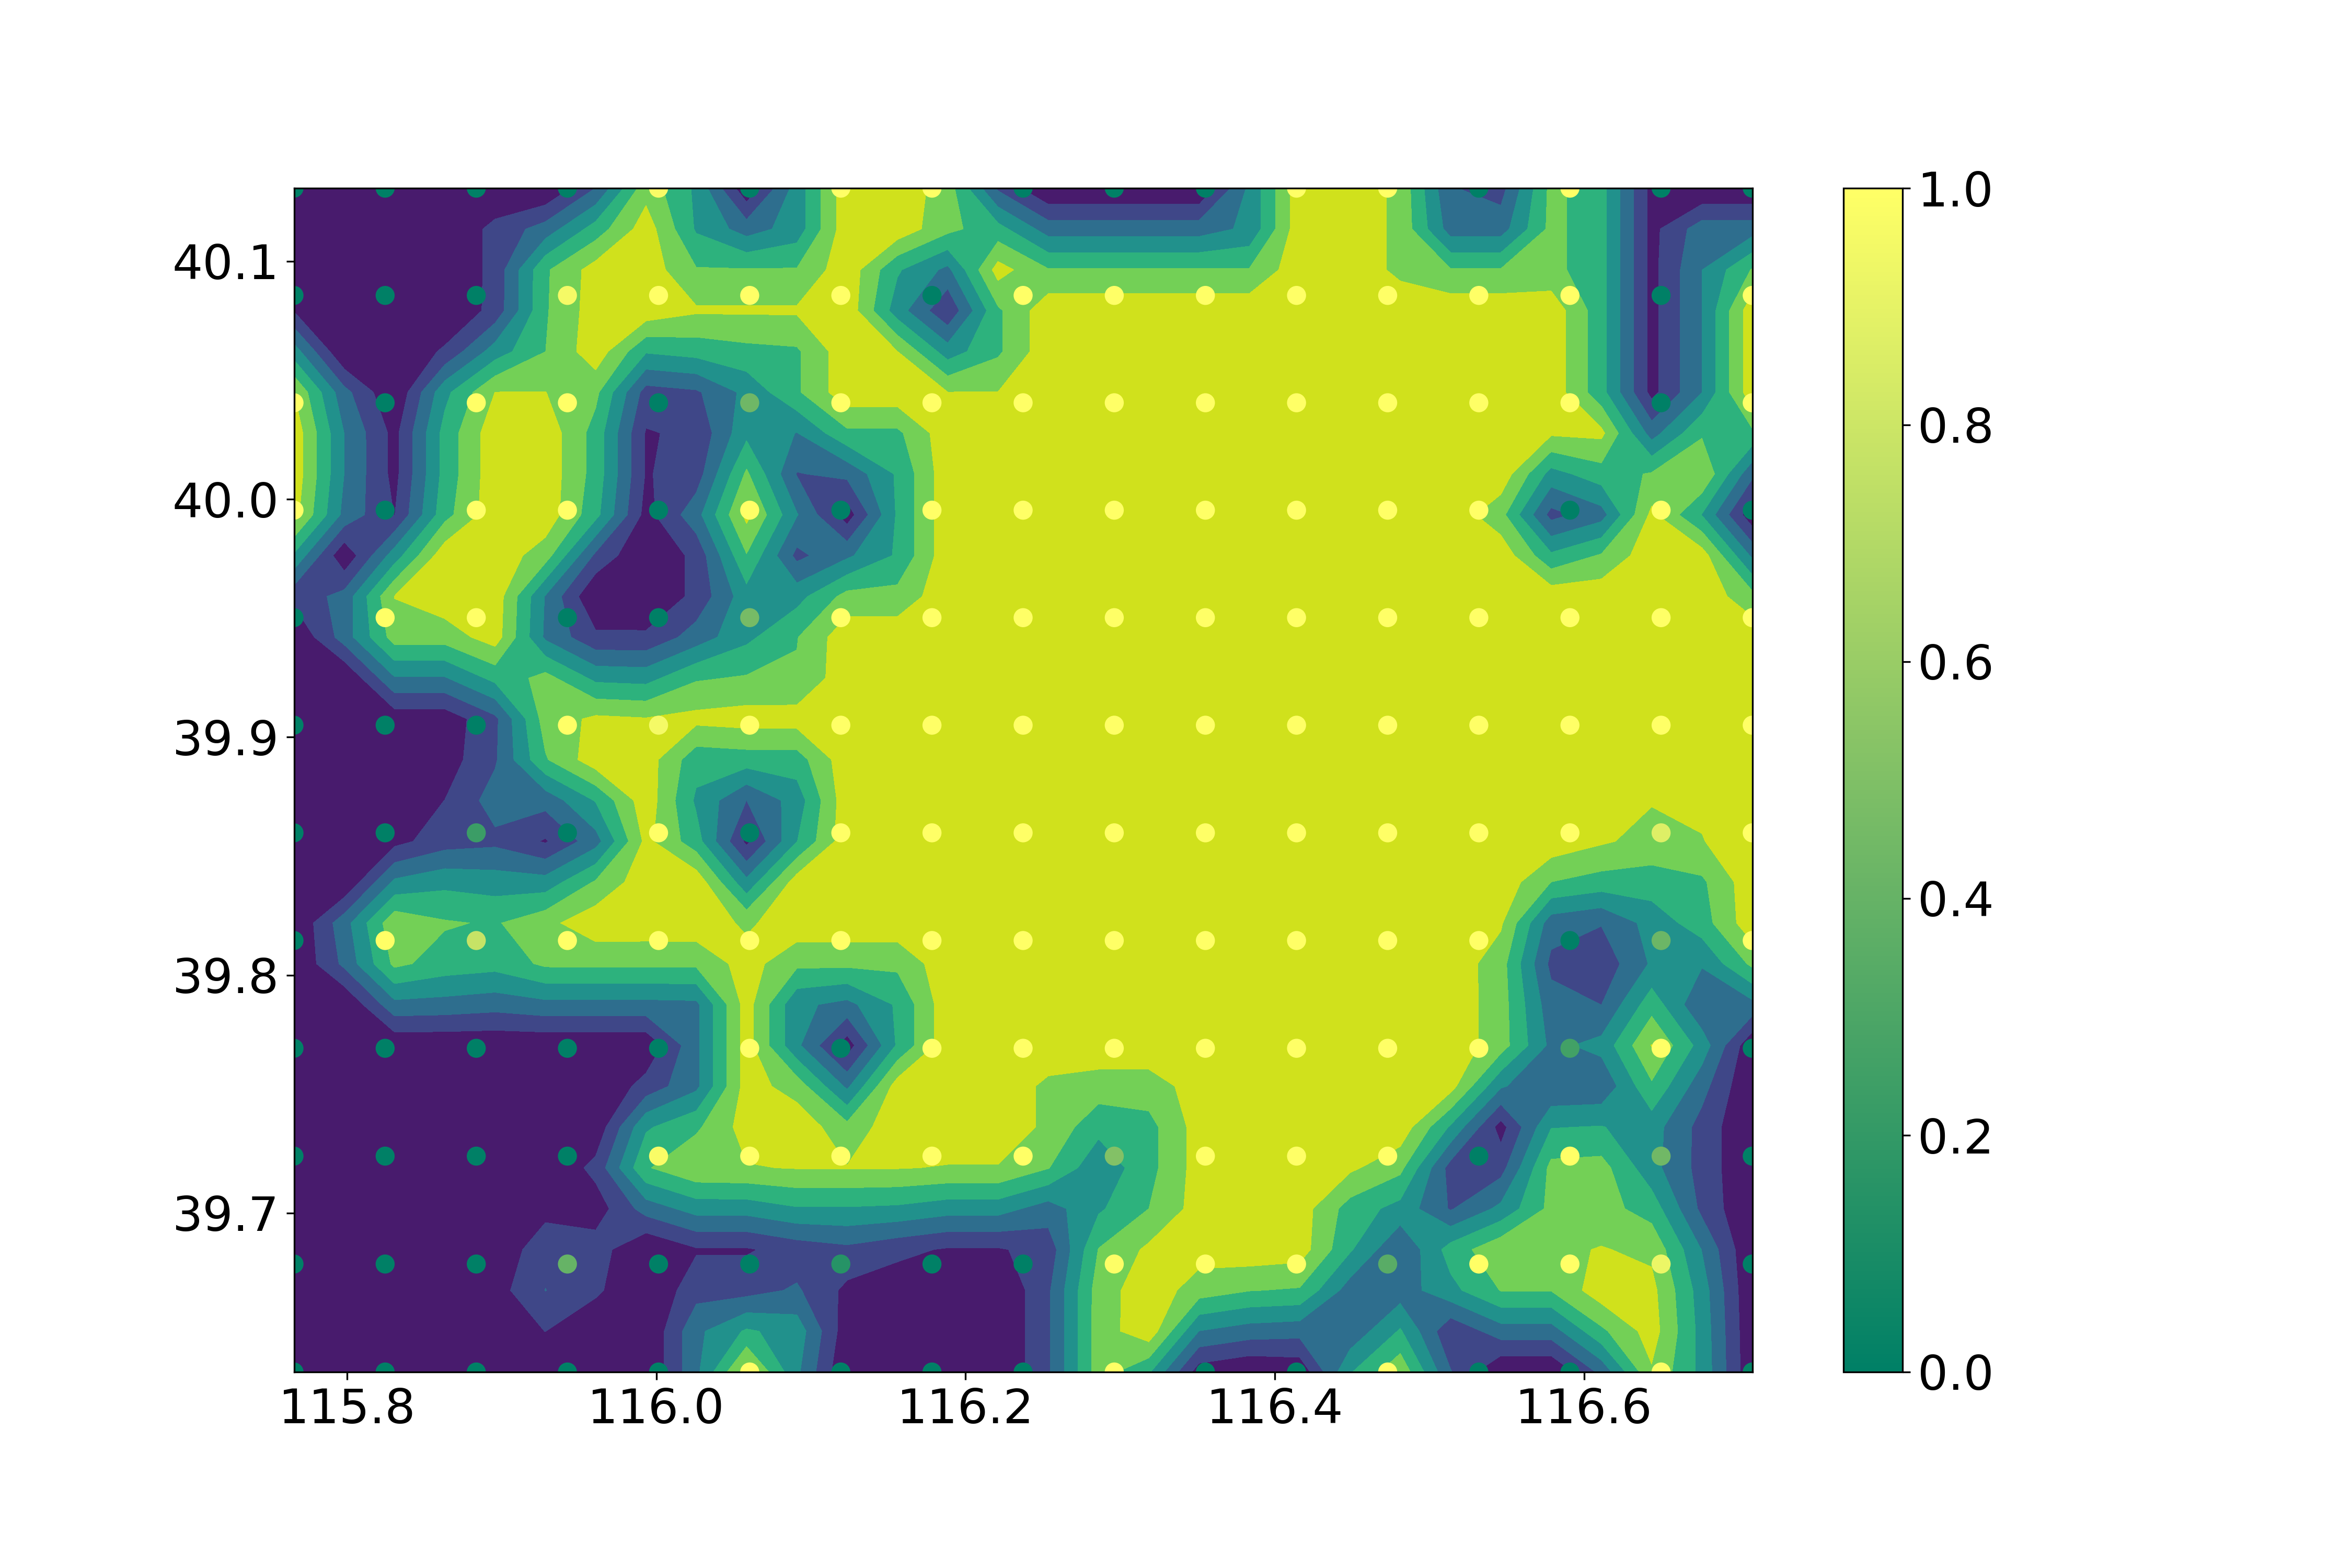
\includegraphics[width=\linewidth]{grid_coverages_0,01_lambda_heatmap.png}
		\caption{Mappa di calore ottenuta per $\lambda = 1/100$}
	\end{subfigure}
	\caption[Risultati griglia, $\lambda = 1/100$]{I risultati ottenuti applicando il modello alla griglia ambientale con $\lambda = 1/100$}
	\label{fig:grid_coverage1}
\end{figure}

\begin{figure}[H]
	\centering
	\begin{subfigure}[b]{\linewidth}
		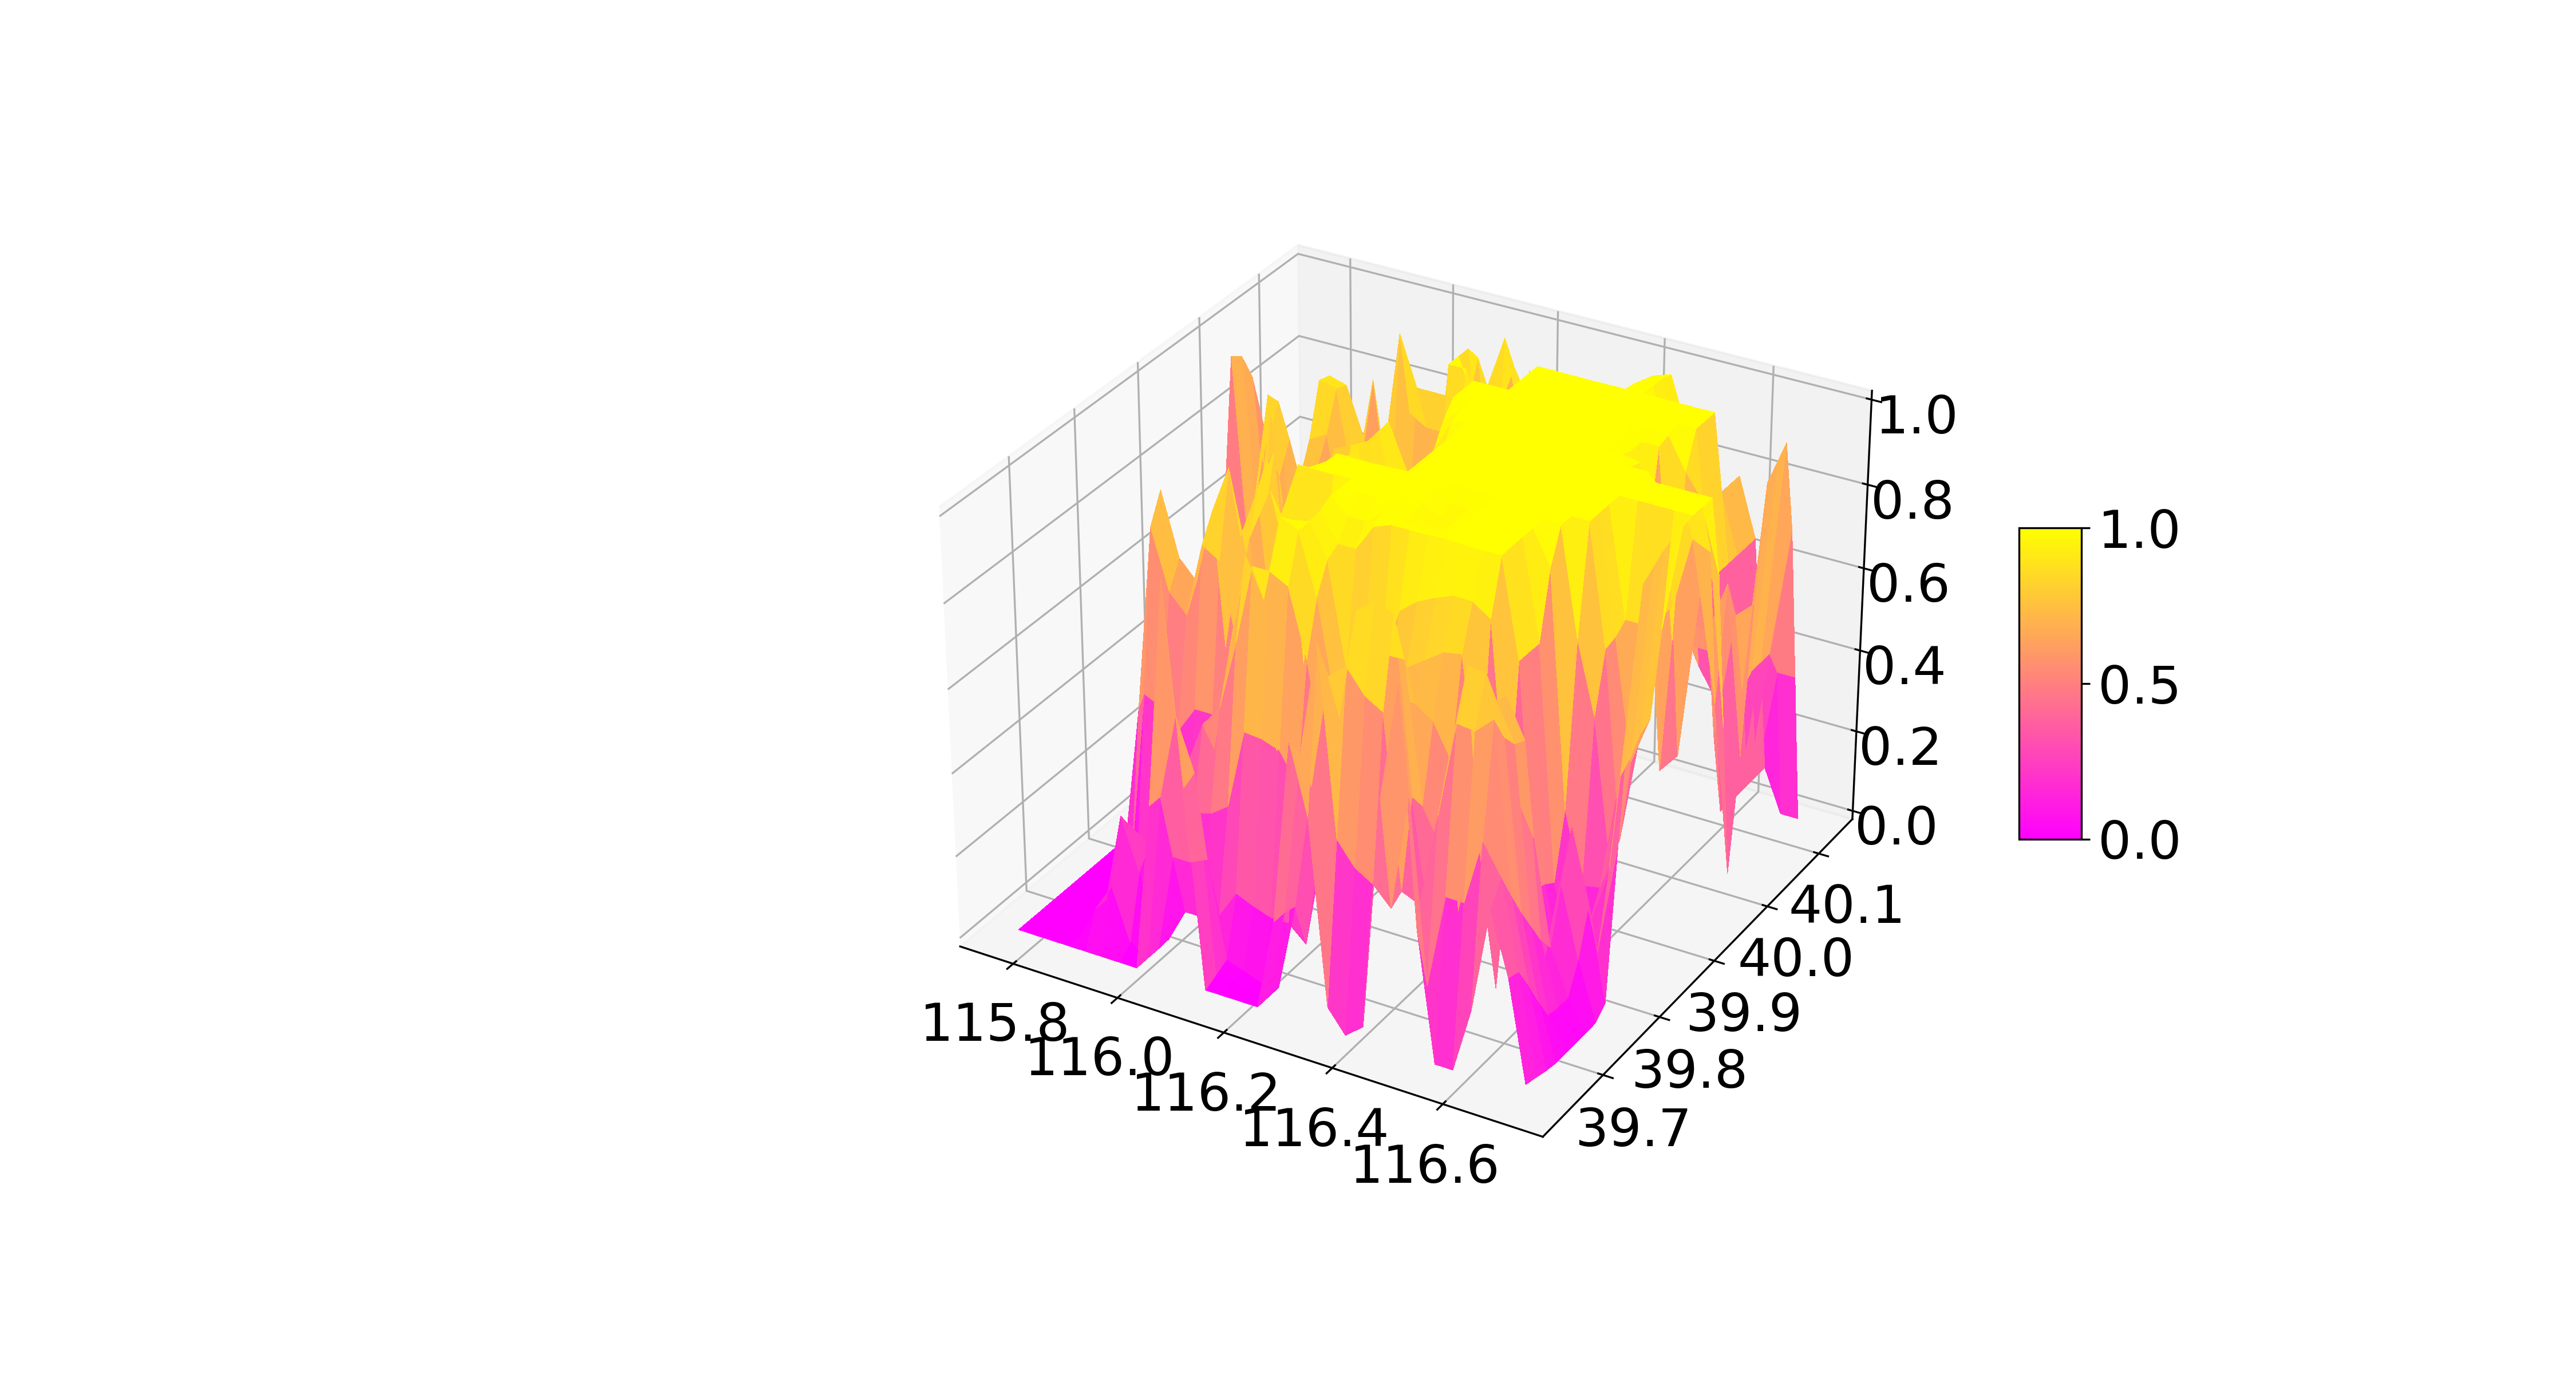
\includegraphics[width=\linewidth]{grid_coverages_0,00333333_lambda_3D_grid.png}
		\caption{Meshgrid ottenuta per $\lambda = 1/300$}
	\end{subfigure}
	\begin{subfigure}[b]{\linewidth}
		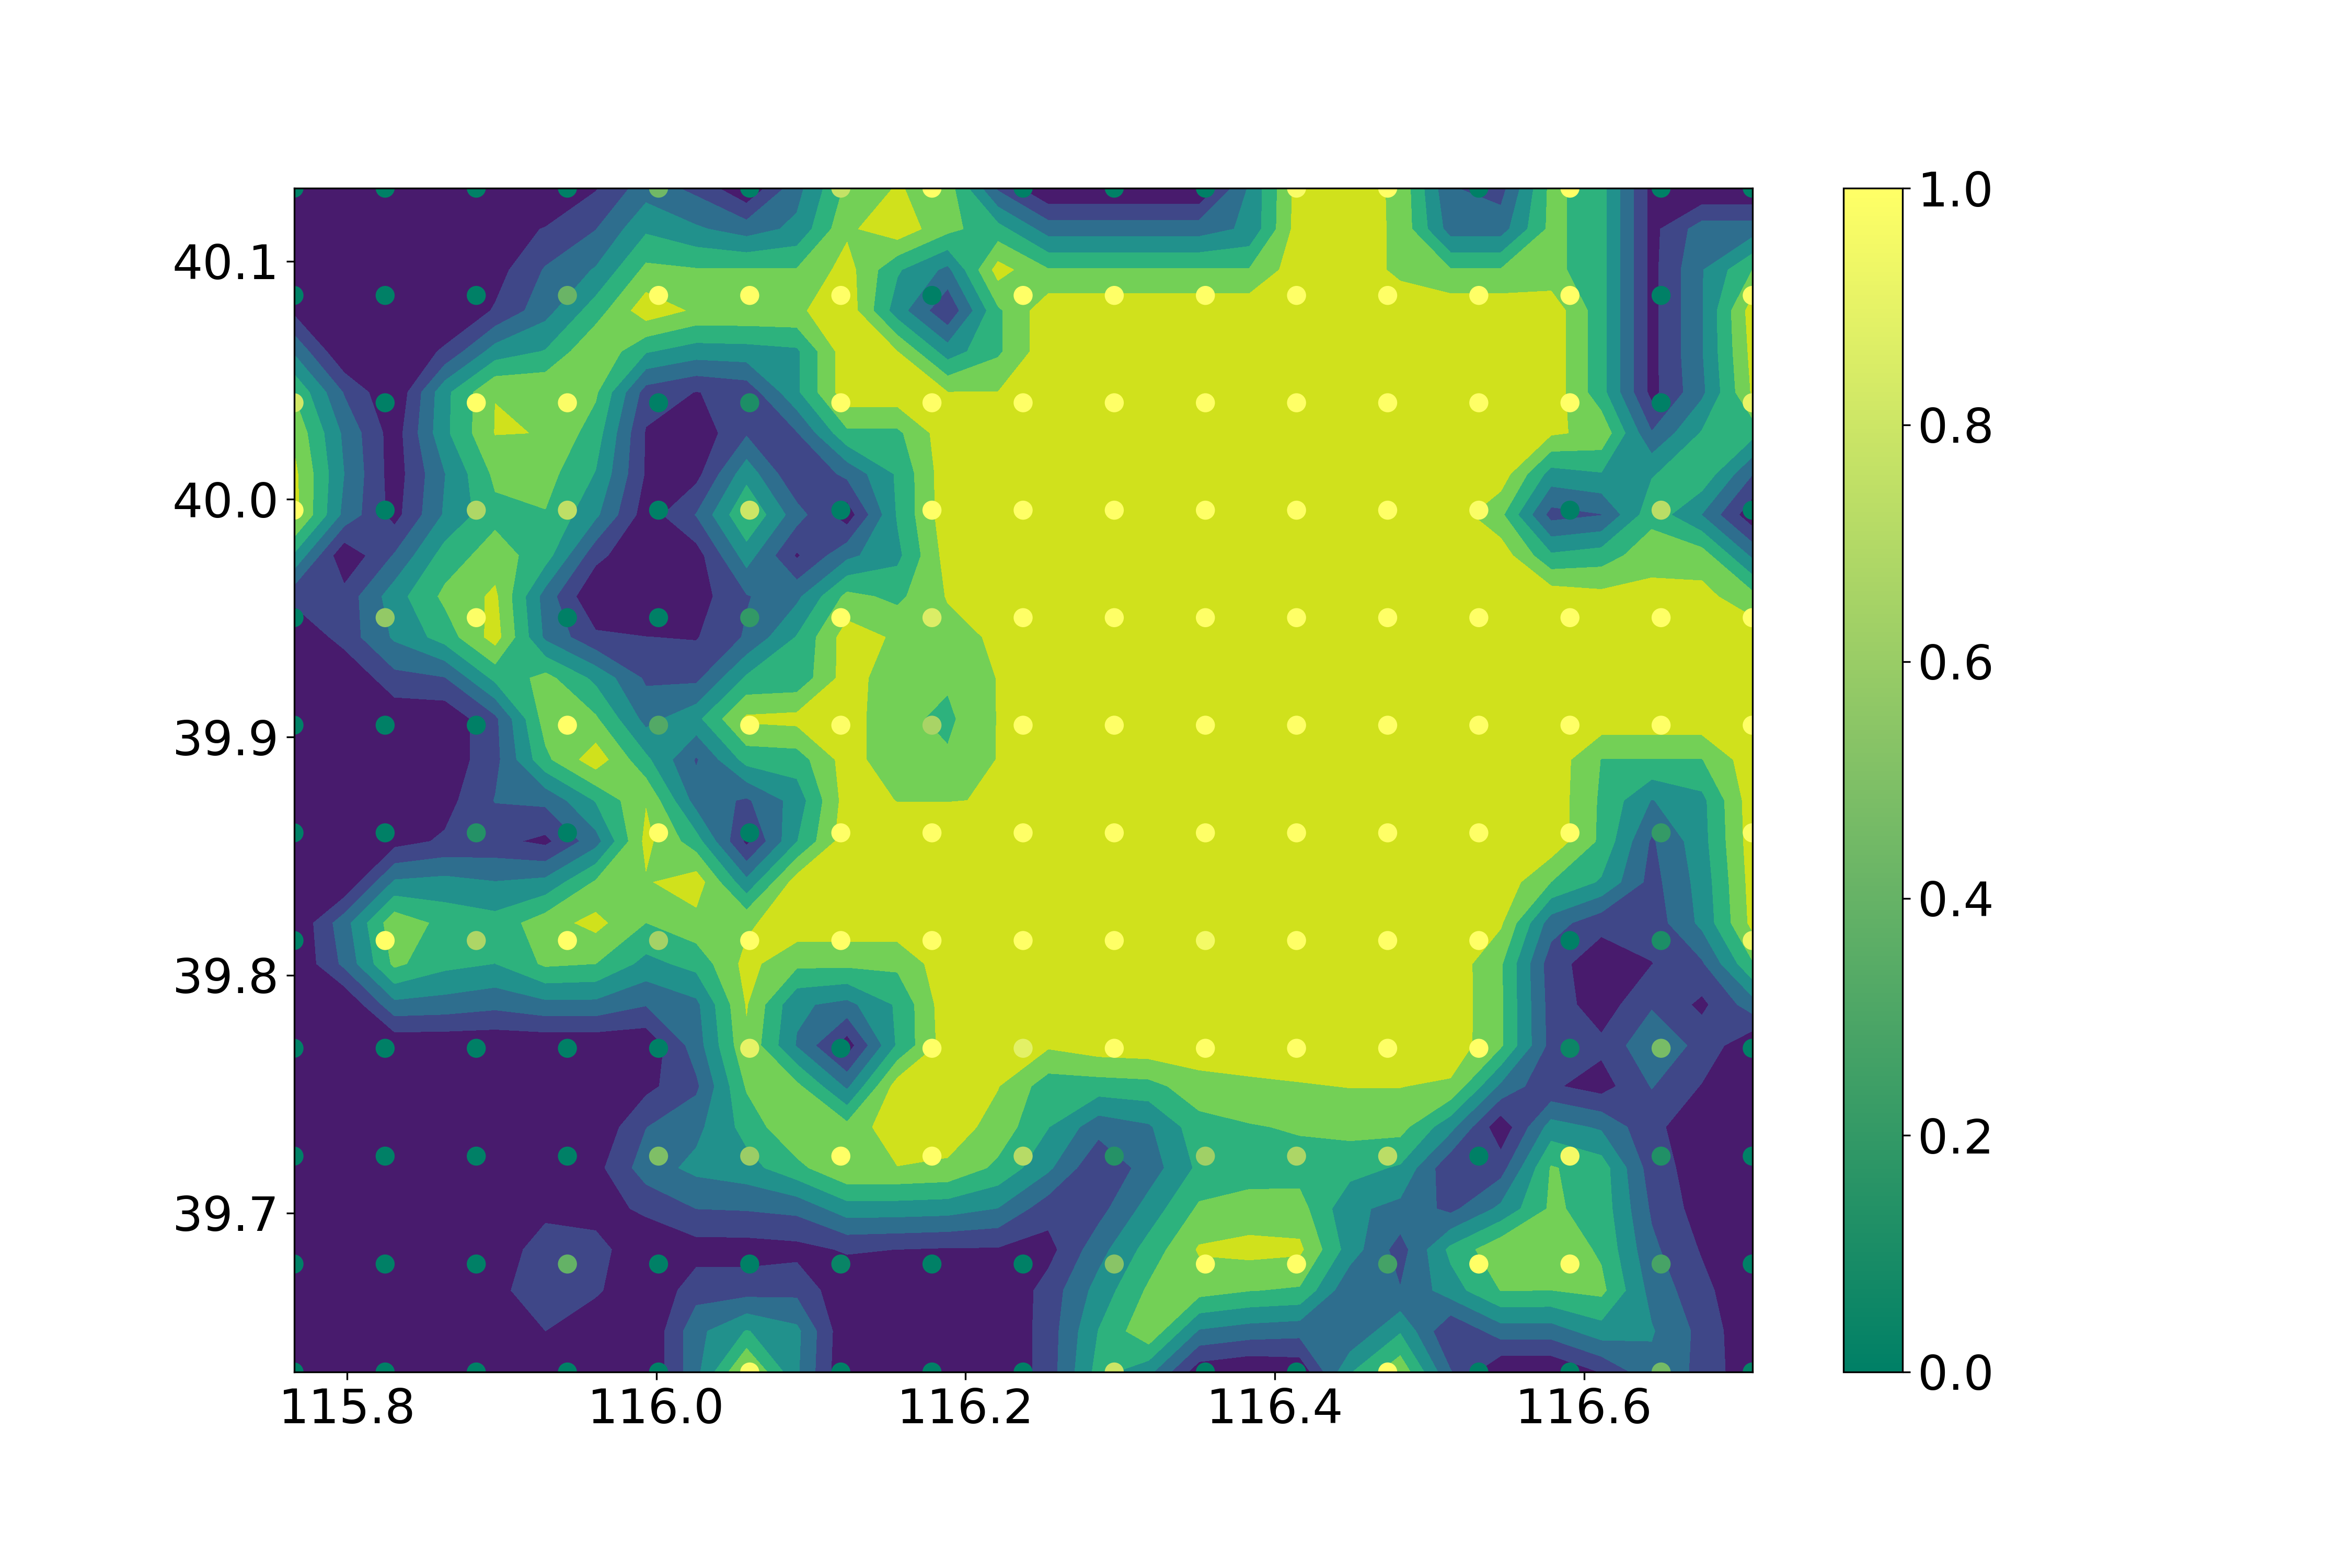
\includegraphics[width=\linewidth]{grid_coverages_0,00333333_lambda_heatmap.png}
		\caption{Mappa di calore ottenuta per $\lambda = 1/300$}
	\end{subfigure}
	\caption[Risultati griglia, $\lambda = 1/300$]{I risultati ottenuti applicando il modello alla griglia ambientale con $\lambda = 1/300$}
	\label{fig:grid_coverage2}
\end{figure}

\begin{figure}[H]
	\centering
	\begin{subfigure}[b]{\linewidth}
		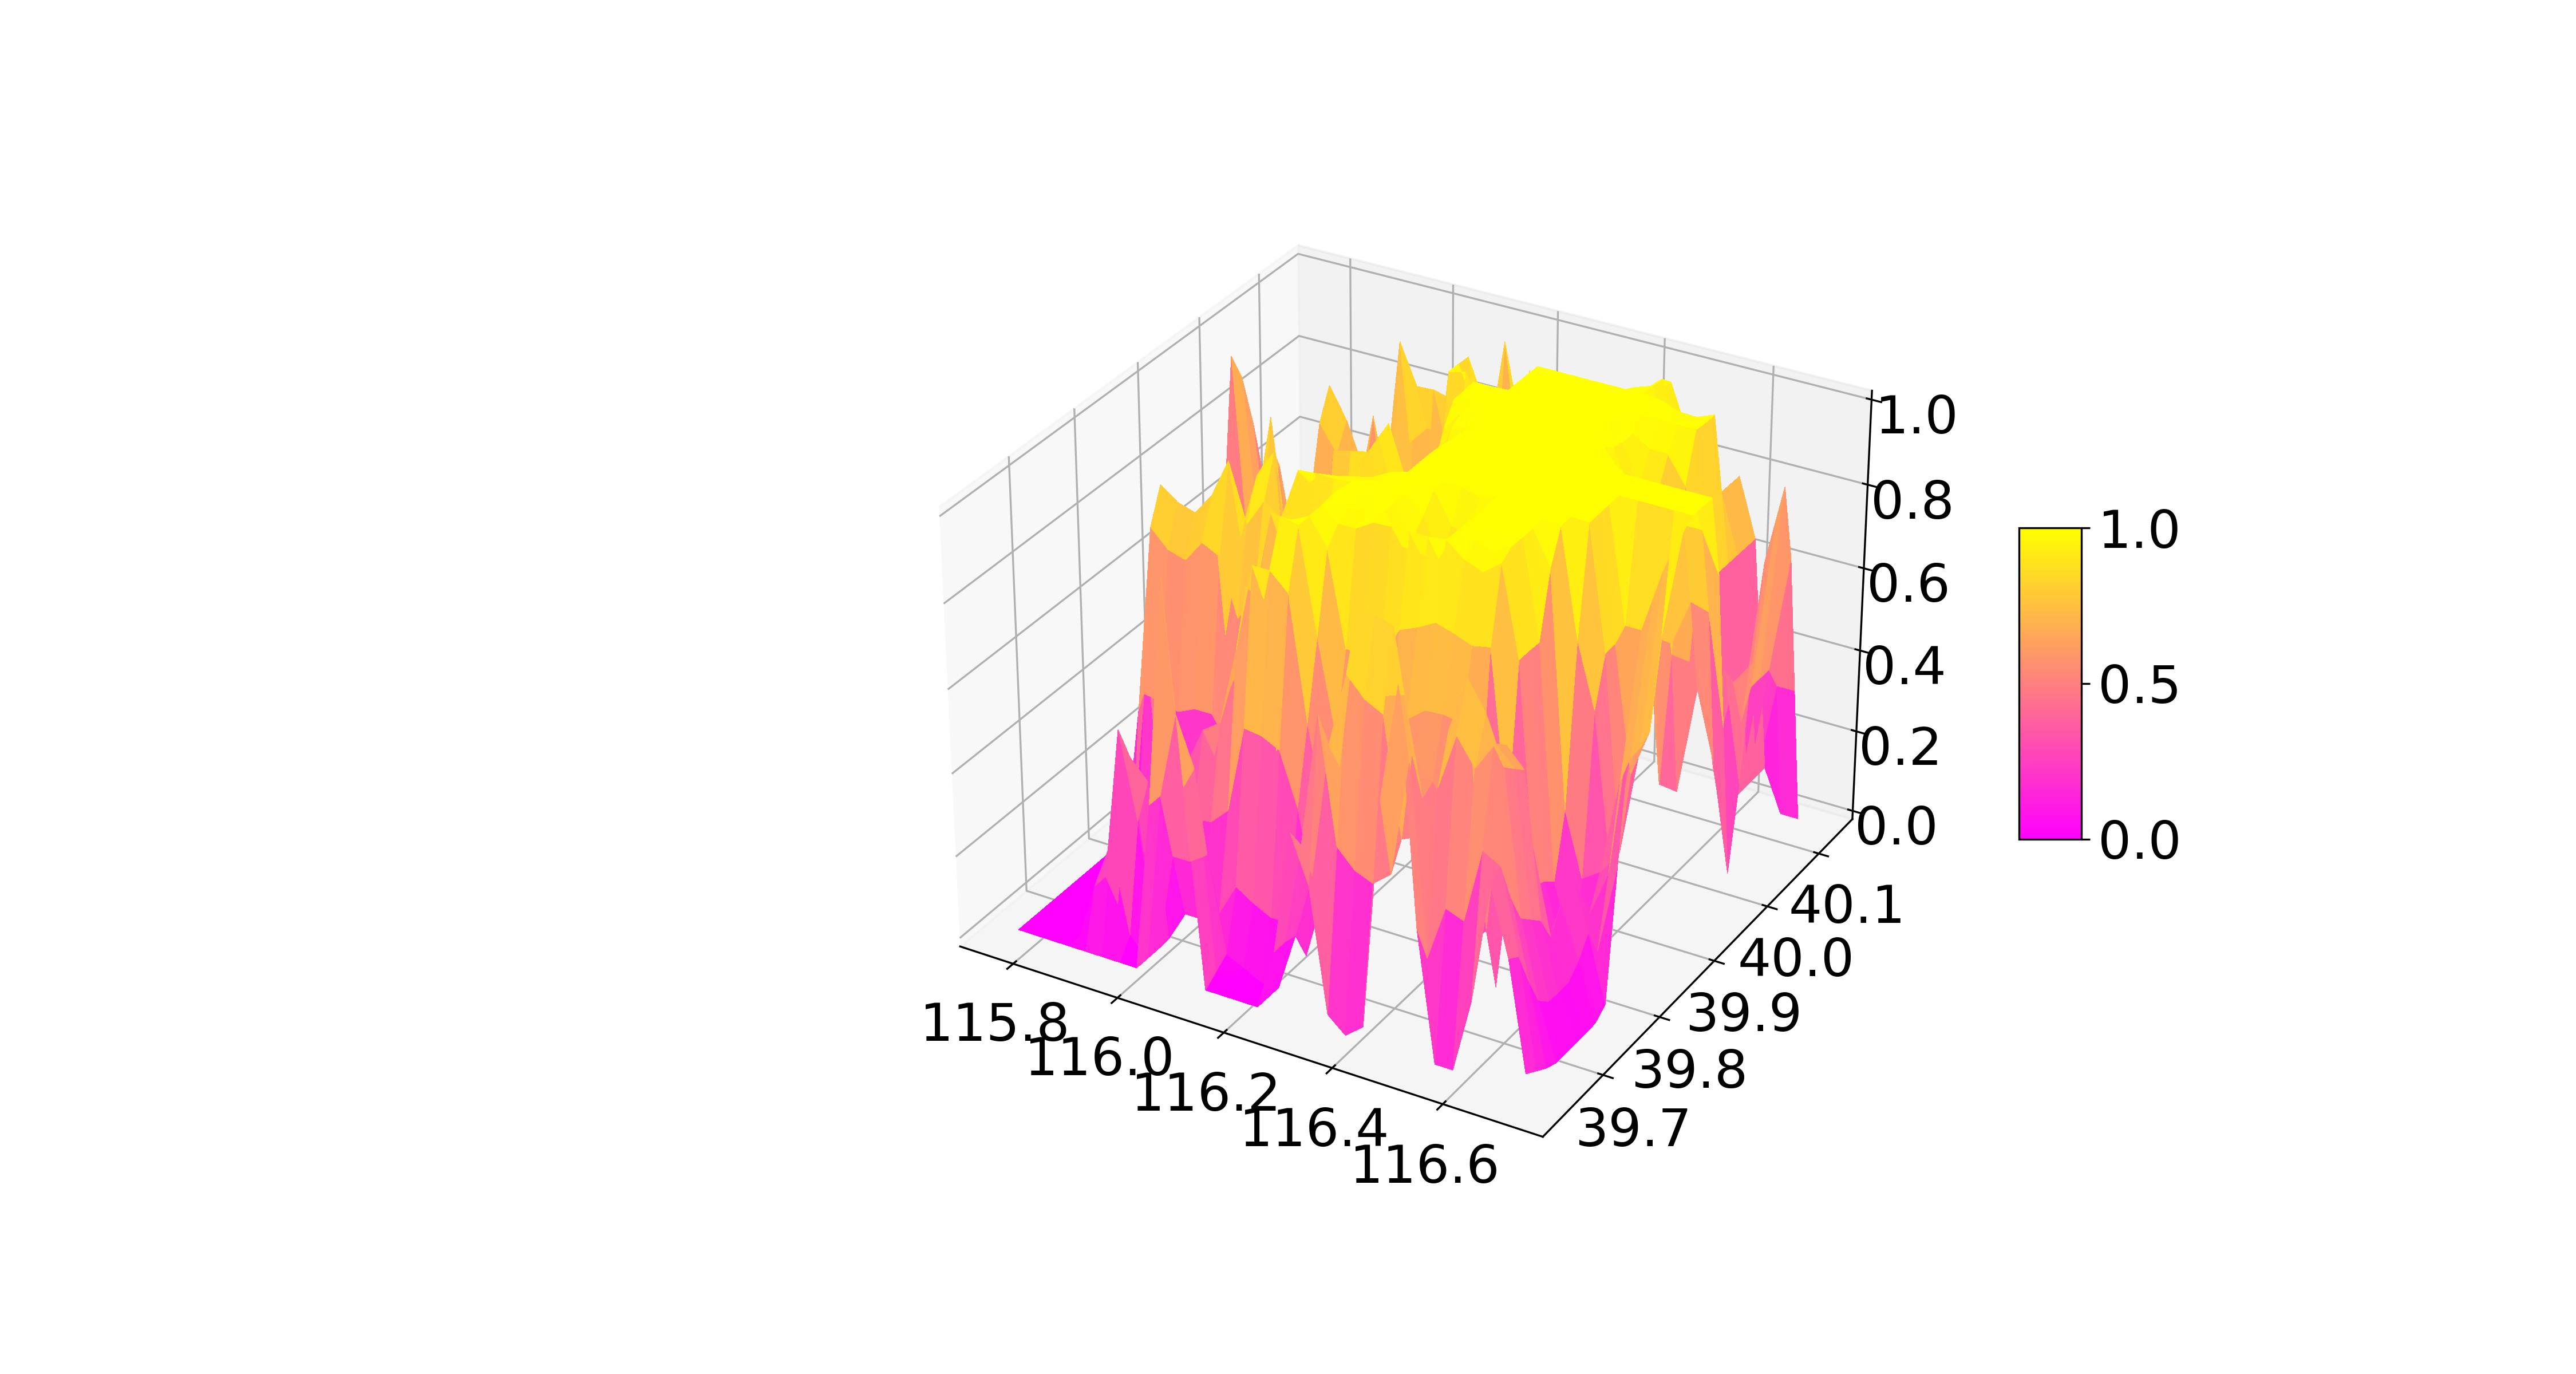
\includegraphics[width=\linewidth]{grid_coverages_0,00142857_lambda_3D_grid.png}
		\caption{Meshgrid ottenuta per $\lambda = 1/700$}
	\end{subfigure}
	\begin{subfigure}[b]{\linewidth}
		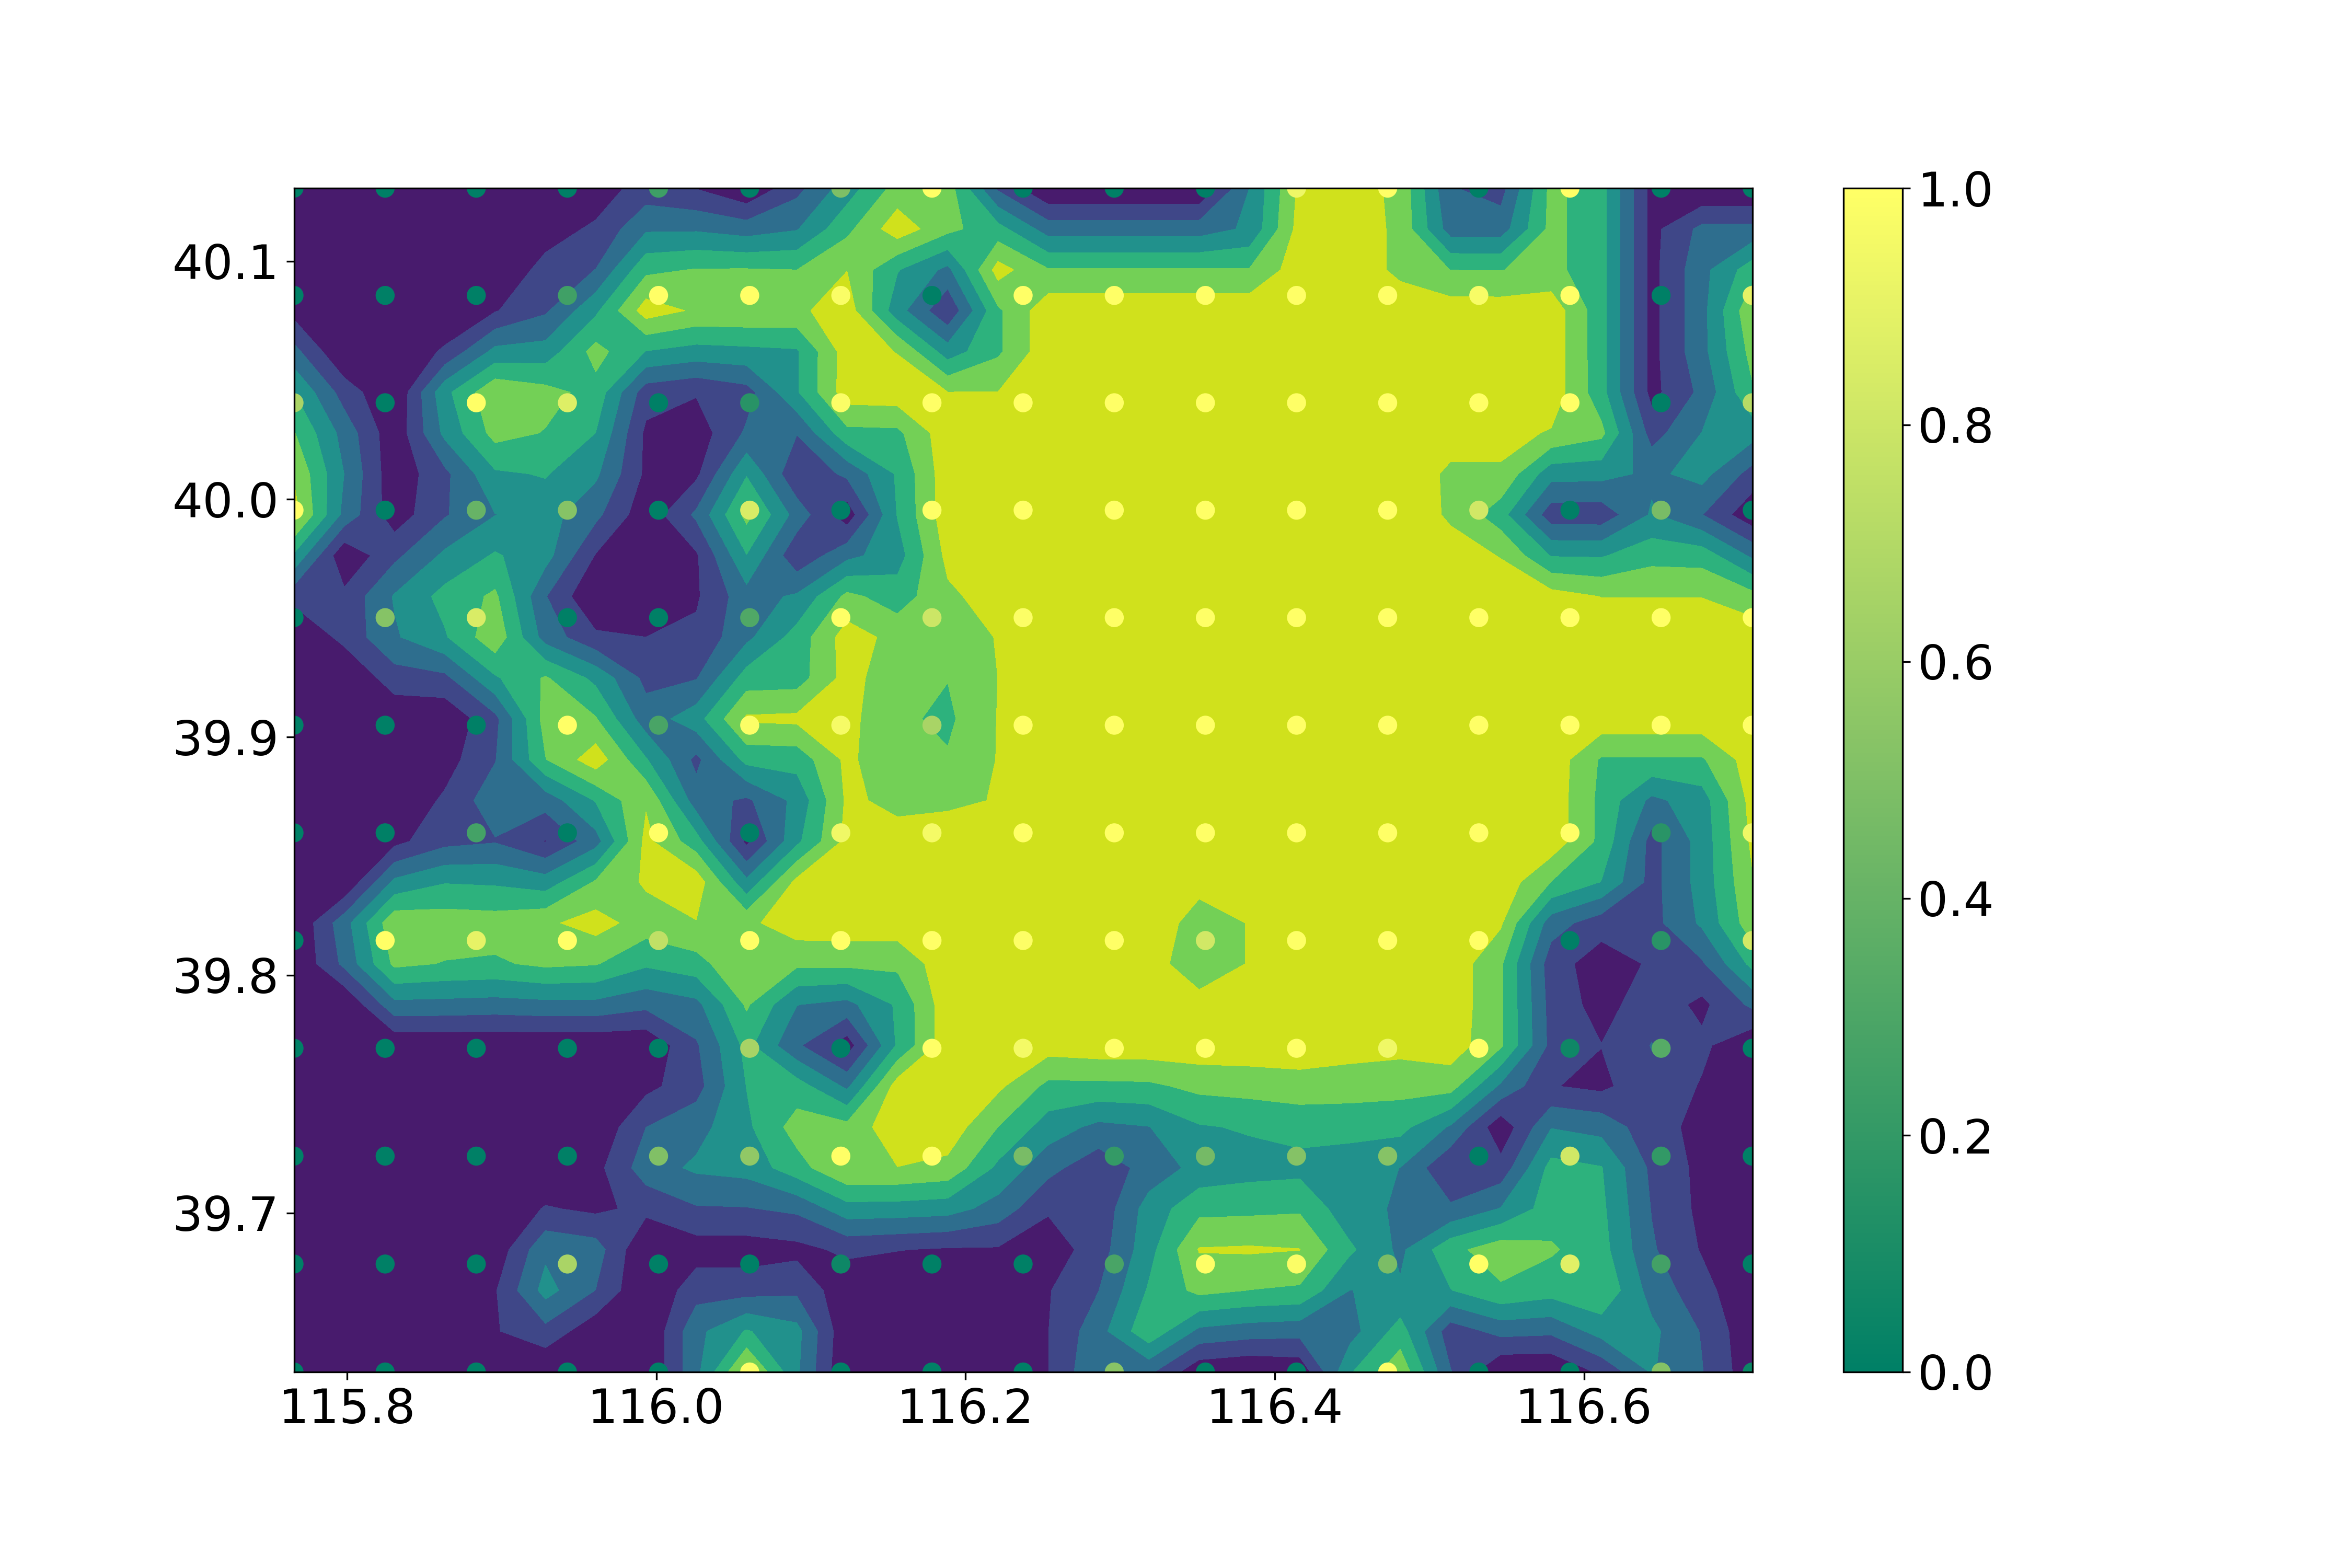
\includegraphics[width=\linewidth]{grid_coverages_0,00142857_lambda_heatmap.png}
		\caption{Mappa di calore ottenuta per $\lambda = 1/700$}
	\end{subfigure}
	\caption[Risultati griglia, $\lambda = 1/700$]{I risultati ottenuti applicando il modello alla griglia ambientale con $\lambda = 1/700$}
	\label{fig:grid_coverage3}
\end{figure}

\section{Flussi di traffico}
Con flusso di traffico si intende l'interazione tra viaggiatori, siano essi a piedi o su un qualsiasi altro mezzo di trasporto, e l'infrastruttura su cui essi si muovono.
I flussi di traffico vengono studiati per migliorare e rendere più efficienti le reti stradali, minimizzando congestioni e massimizzando il throughput della infrastruttura in termini di capacità effettiva di spostamento.

Riguardo al monitoraggio di tali flussi, ci siamo avvalsi di un data set con le coordinate geografiche di tutte le stazioni della metropolitana di Pechino estratto per mezzo di OSMnx \cite{osmnx}. Ipotizziamo che tali snodi principali siamo molto trafficati e siano visitati da una moltitudine di persone. Questo specifico scenario ci permette di valutare quale sia la portata del traffico umano attraverso questi luoghi. 

Il monitoraggio tramite MCS dei flussi di traffico, permette di raccogliere dati reali dalle infrastrutture di una Smart City permettendo a chi la gestisce di applicare nuove e migliori politiche urbanistiche e di gestione delle infrastrutture.

\subsection{OSMnx e metropolitane di Pechino}
Grazie alla funzione \textit{pois\_from\_point()} appartenente a OSMnx \cite{osmnx}, abbiamo estratto dal database di OpenStreetMap le coordinate GPS delle stazioni della metropolitana in un raggio di 50Km dal centro di Pechino.
Dopo aver ripulito il dataset estratto, abbiamo ottenuto un totale di 331 punti che abbiamo poi serializzato per il successivo calcolo della Data Coverage.

\subsection{Visualizzazione delle stazioni della metropolitana}
La Figura \ref{fig:subway} mostra le stazioni della metropolitana considerate, stampate grazie a folium \cite{folium}.
Analogamente alla griglia, la mappa ha in sovraimpressione alcune delle traiettorie del dataset. I cerchi blu rappresentano le singole stazioni della metropolitana.

\begin{figure}[H]
	\centering 
	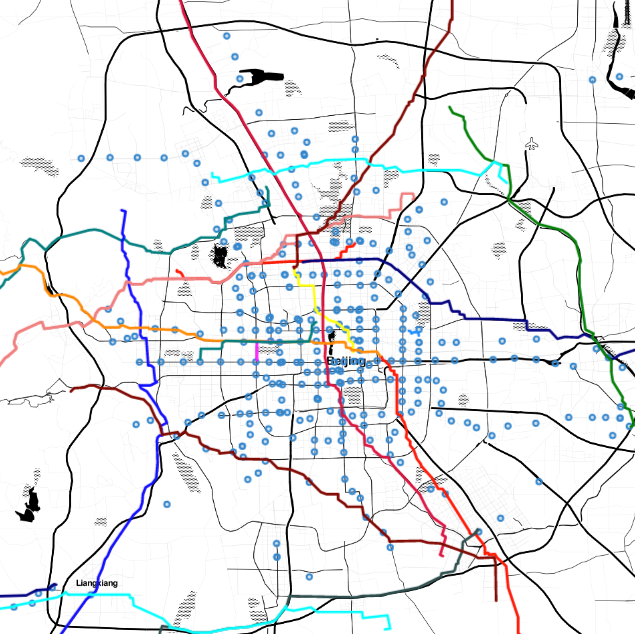
\includegraphics[width=\linewidth]{subway_folium.png}
	\caption[Mappa delle stazioni della metropolitana]{Le stazioni della metropolitana stampate grazie a folium}
	\label{fig:subway}
\end{figure}

\subsection{Risultati del modello di coverage}
Le Figure \ref{fig:subway_coverage1}, \ref{fig:subway_coverage2}, e \ref{fig:subway_coverage3}, mostrano i risultati ottenuti applicando il modello con differenti valori di lambda sulle uscite della metropolitana estratte per mezzo di OSMnx \cite{osmnx}. 

\begin{figure}[H]
	\centering
	\begin{subfigure}[b]{\linewidth}
		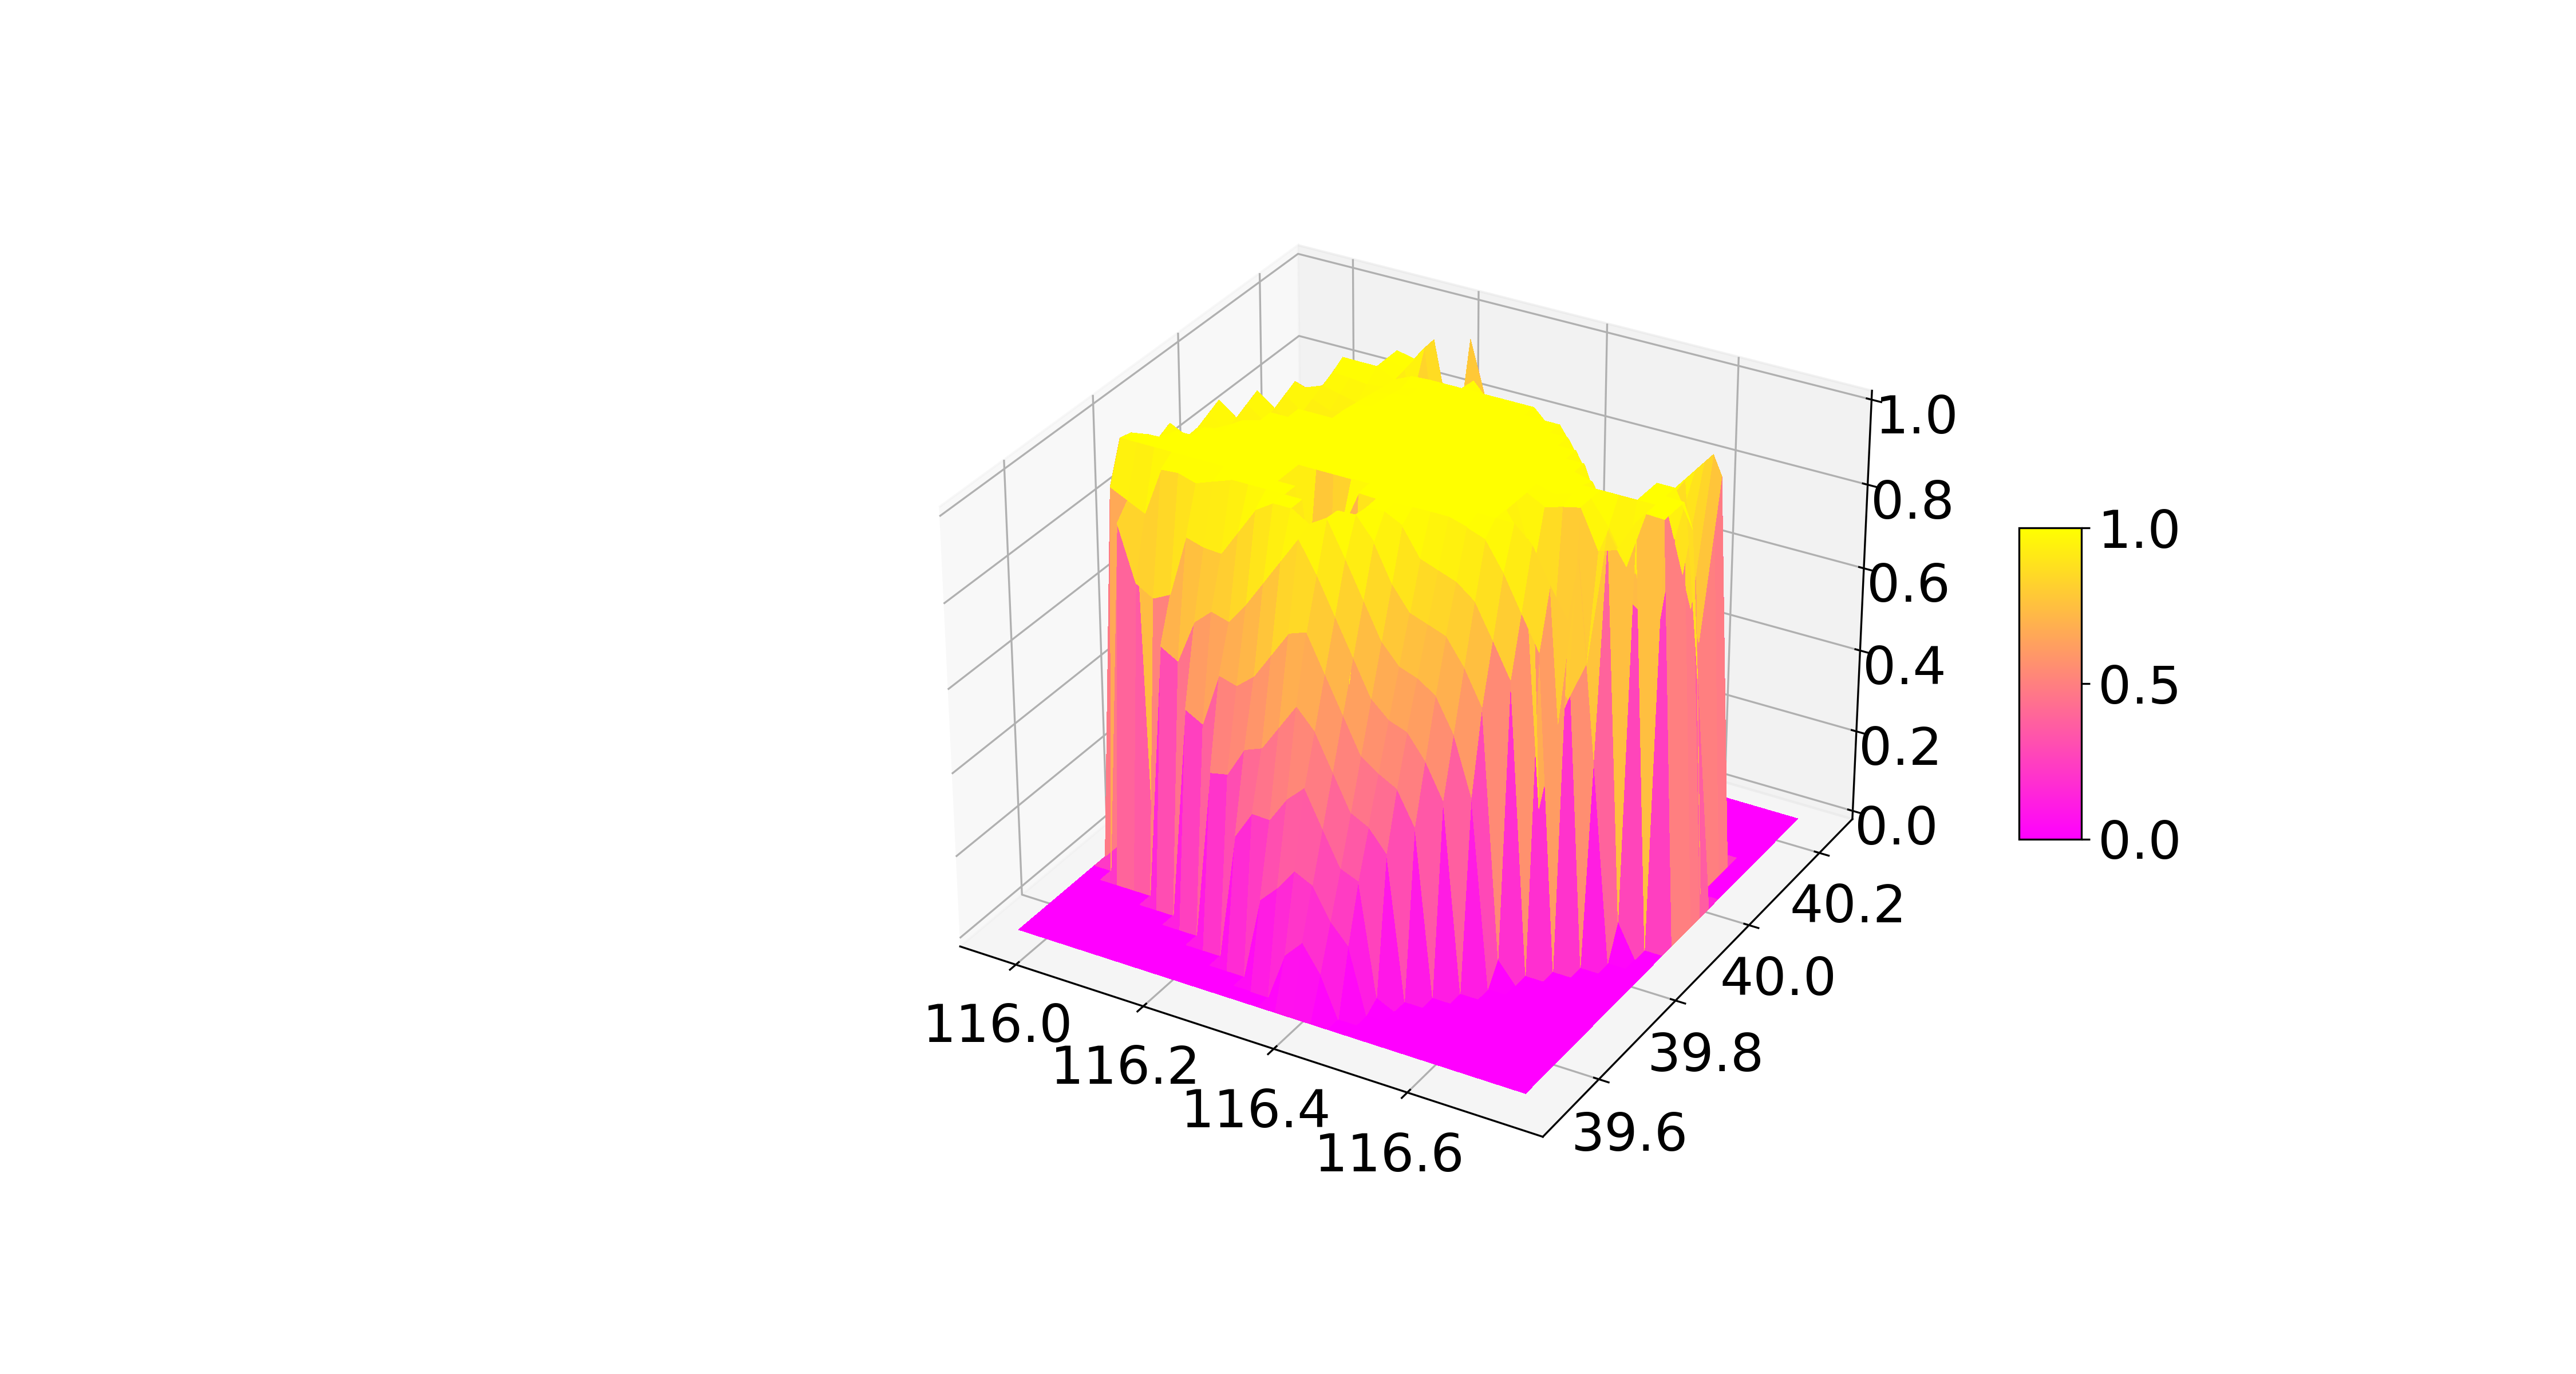
\includegraphics[width=\linewidth]{subway_coverages_0,01_lambda_3D_grid.png}
		\caption{Meshgrid ottenuta per $\lambda = 1/100$}
	\end{subfigure}
	\begin{subfigure}[b]{\linewidth}
		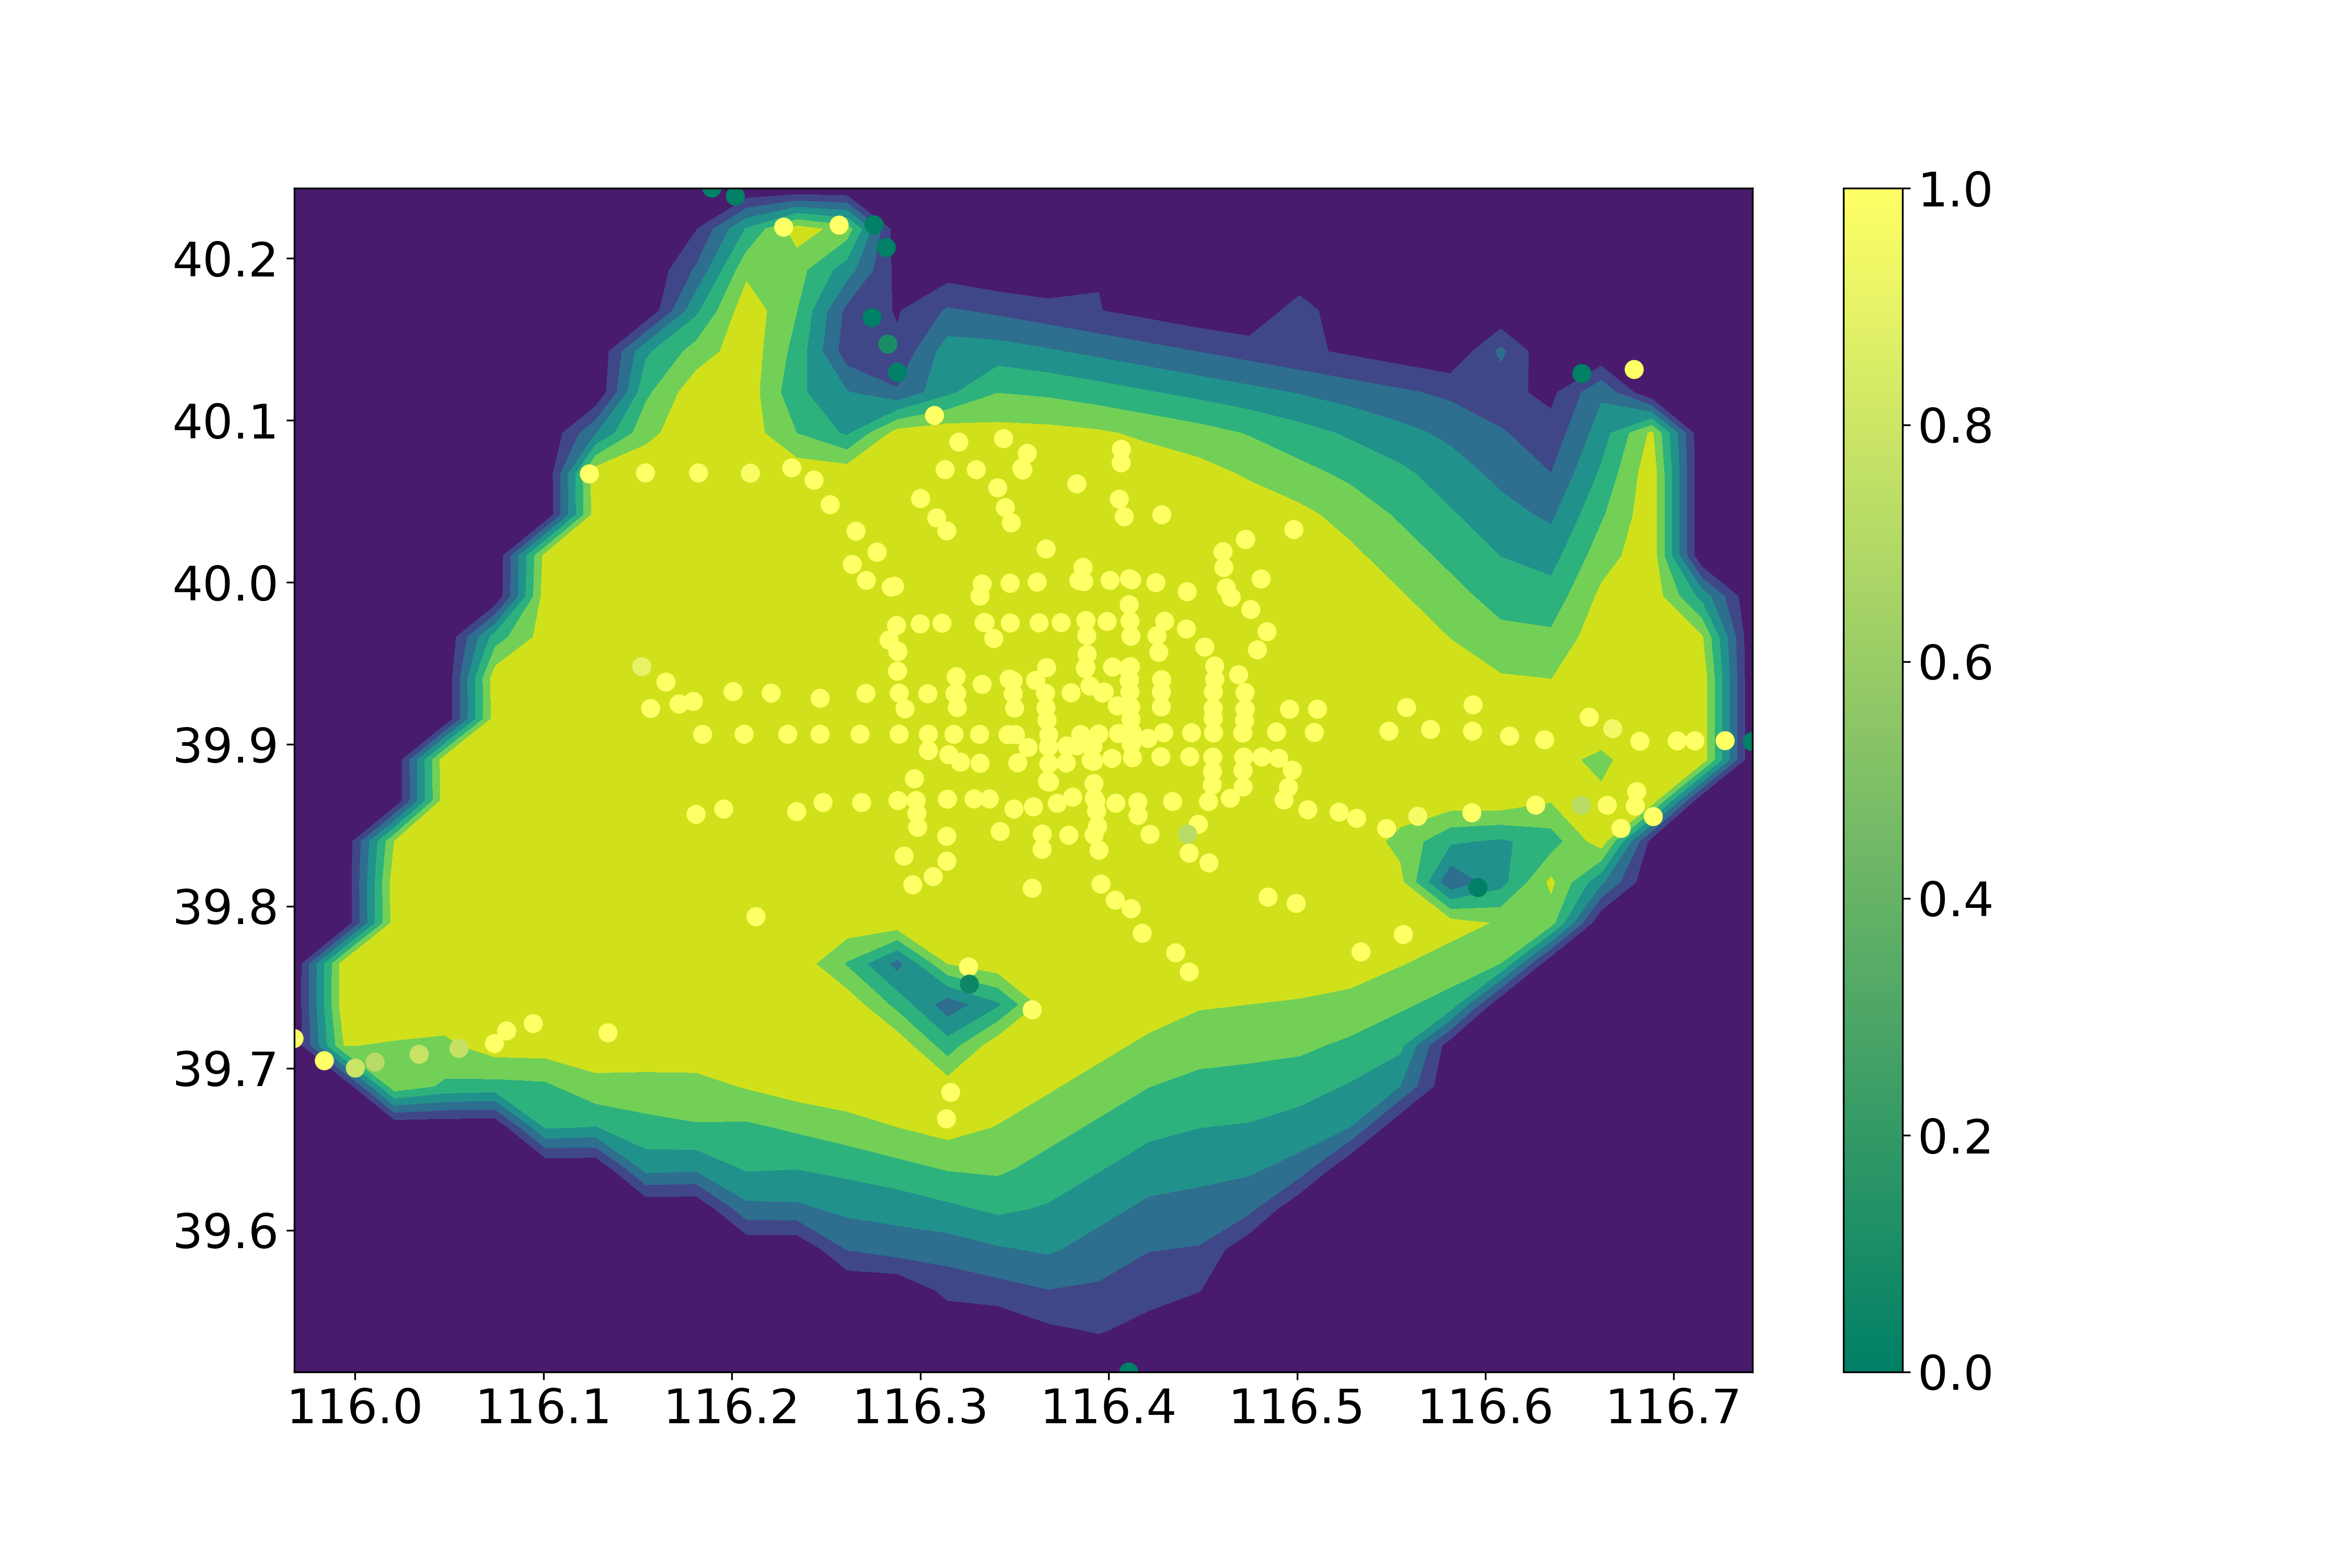
\includegraphics[width=\linewidth]{subway_coverages_0,01_lambda_heatmap.png}
		\caption{Mappa di calore ottenuta per $\lambda = 1/100$}
	\end{subfigure}
	\caption[Risultati metropolitana, $\lambda = 1/100$]{I risultati ottenuti applicando il modello alle uscite della metropolitana con $\lambda = 1/100$}
	\label{fig:subway_coverage1}
\end{figure}

\begin{figure}[H]
	\centering
	\begin{subfigure}[b]{\linewidth}
		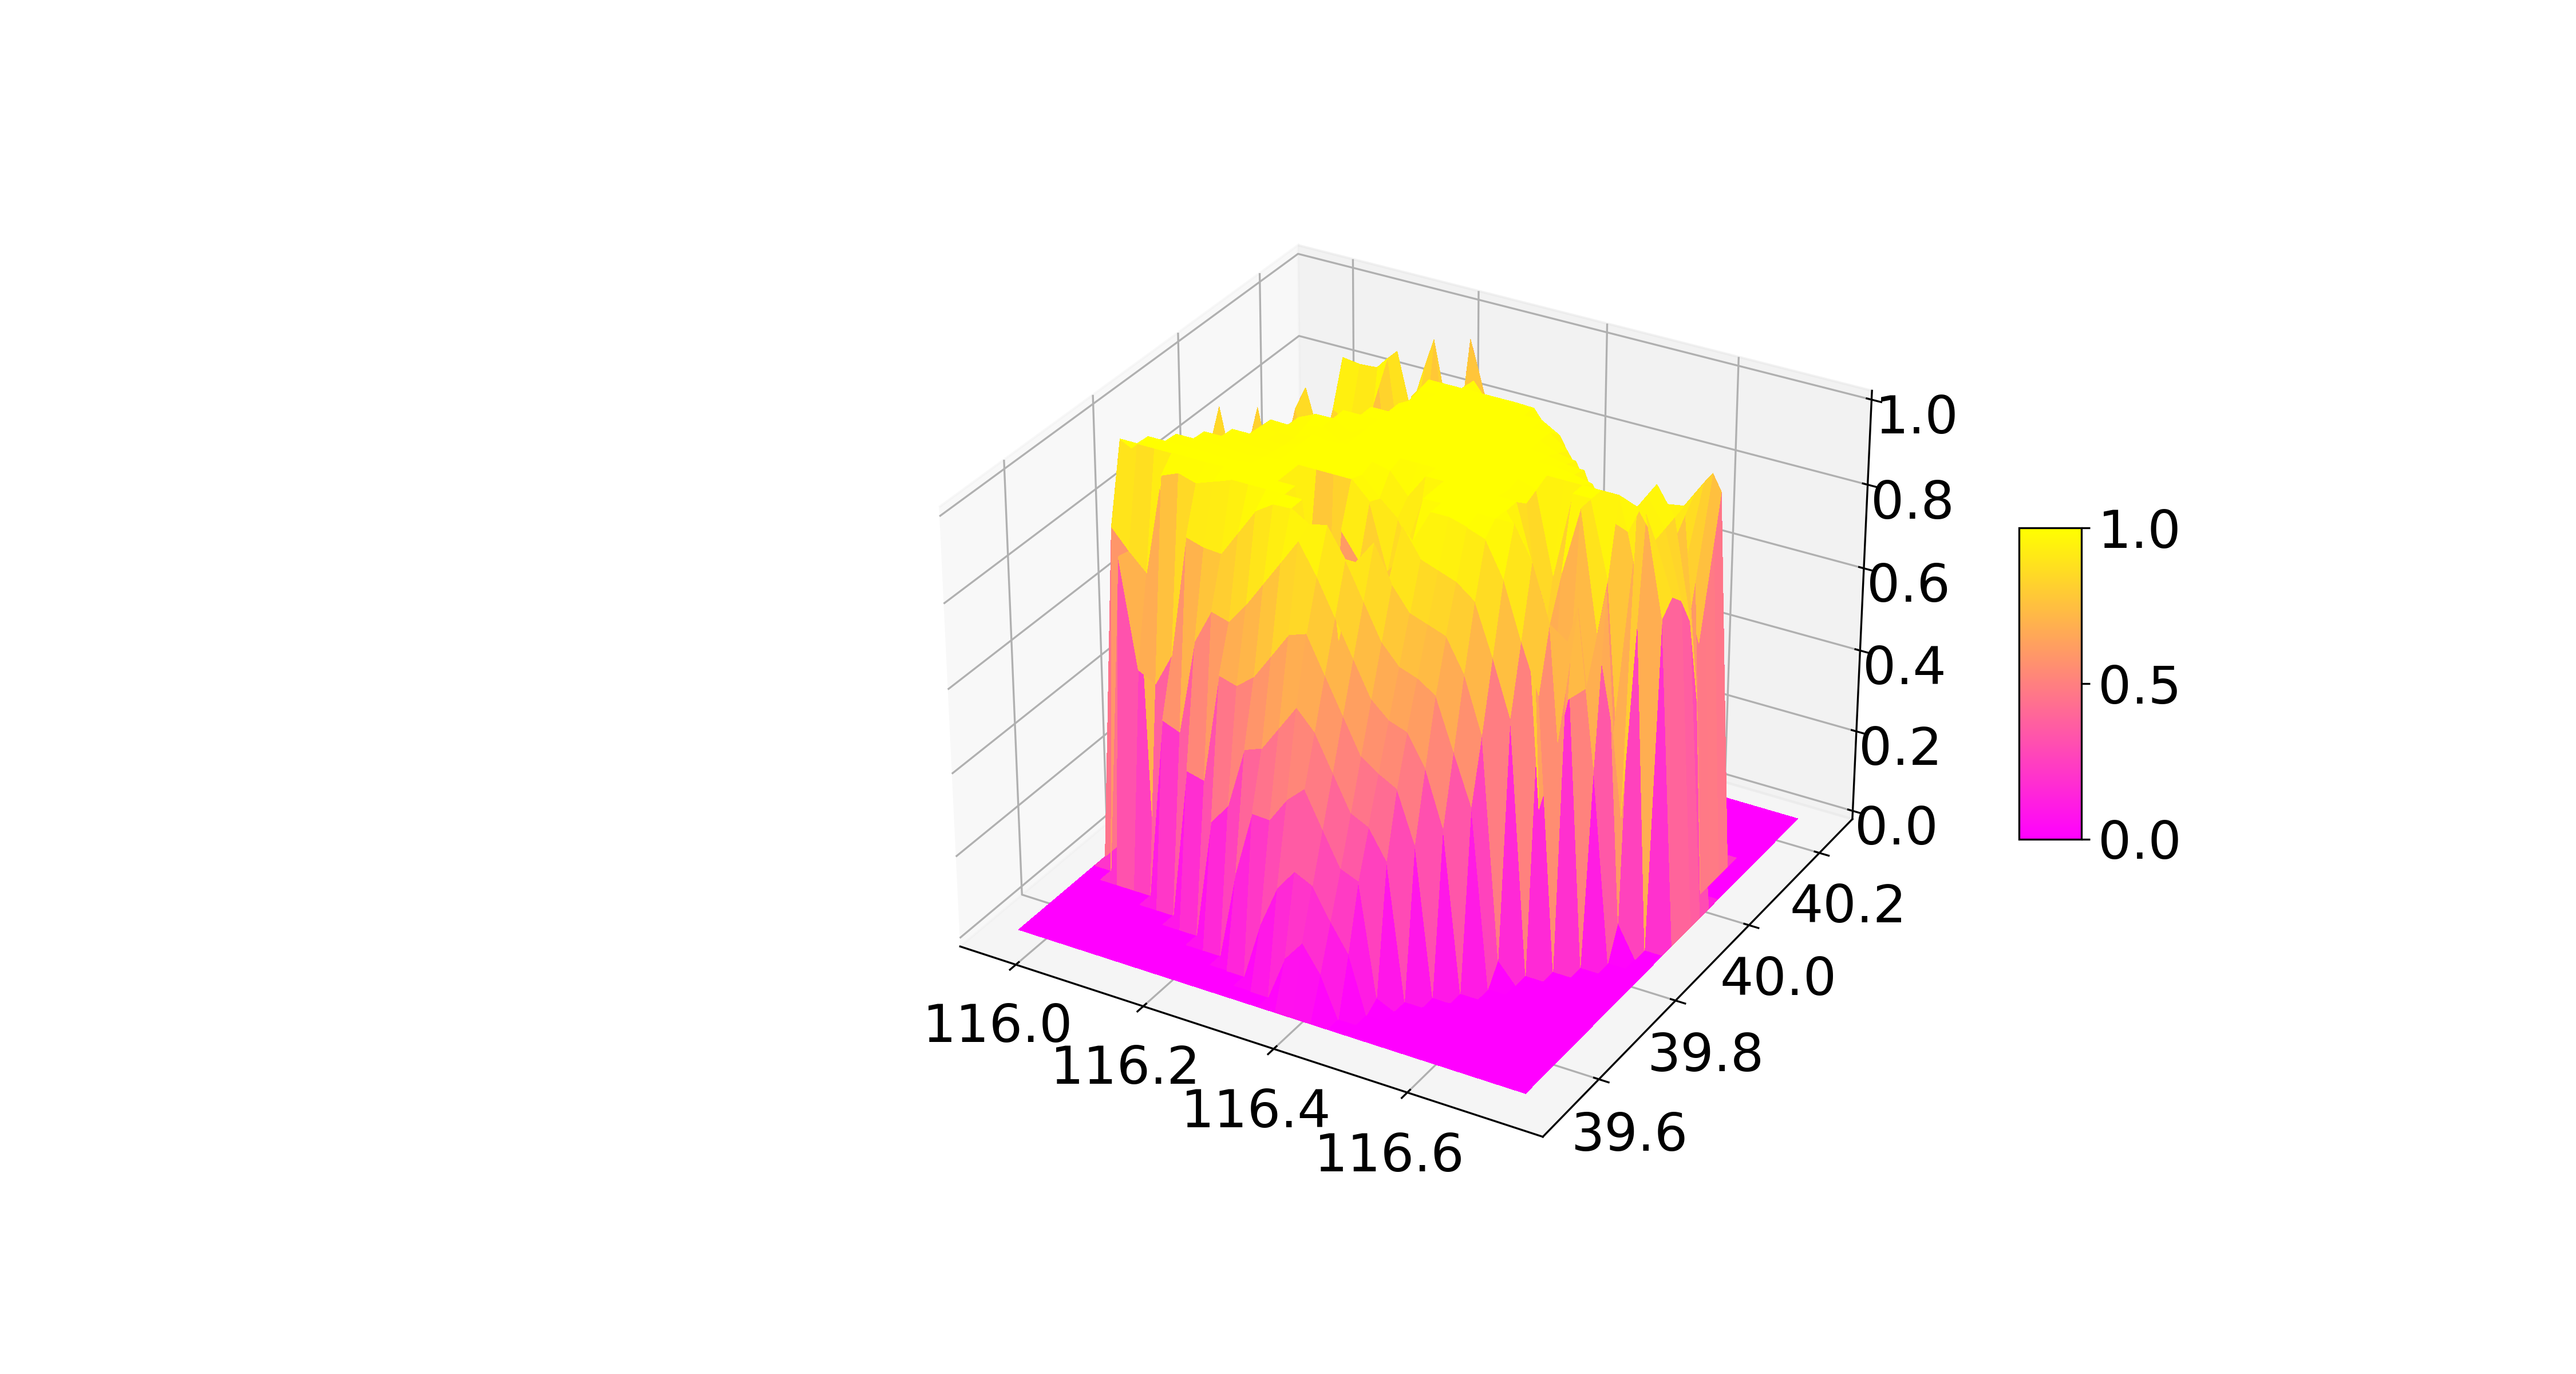
\includegraphics[width=\linewidth]{subway_coverages_0,00333333_lambda_3D_grid.png}
		\caption{Meshgrid ottenuta per $\lambda = 1/300$}
	\end{subfigure}
	\begin{subfigure}[b]{\linewidth}
		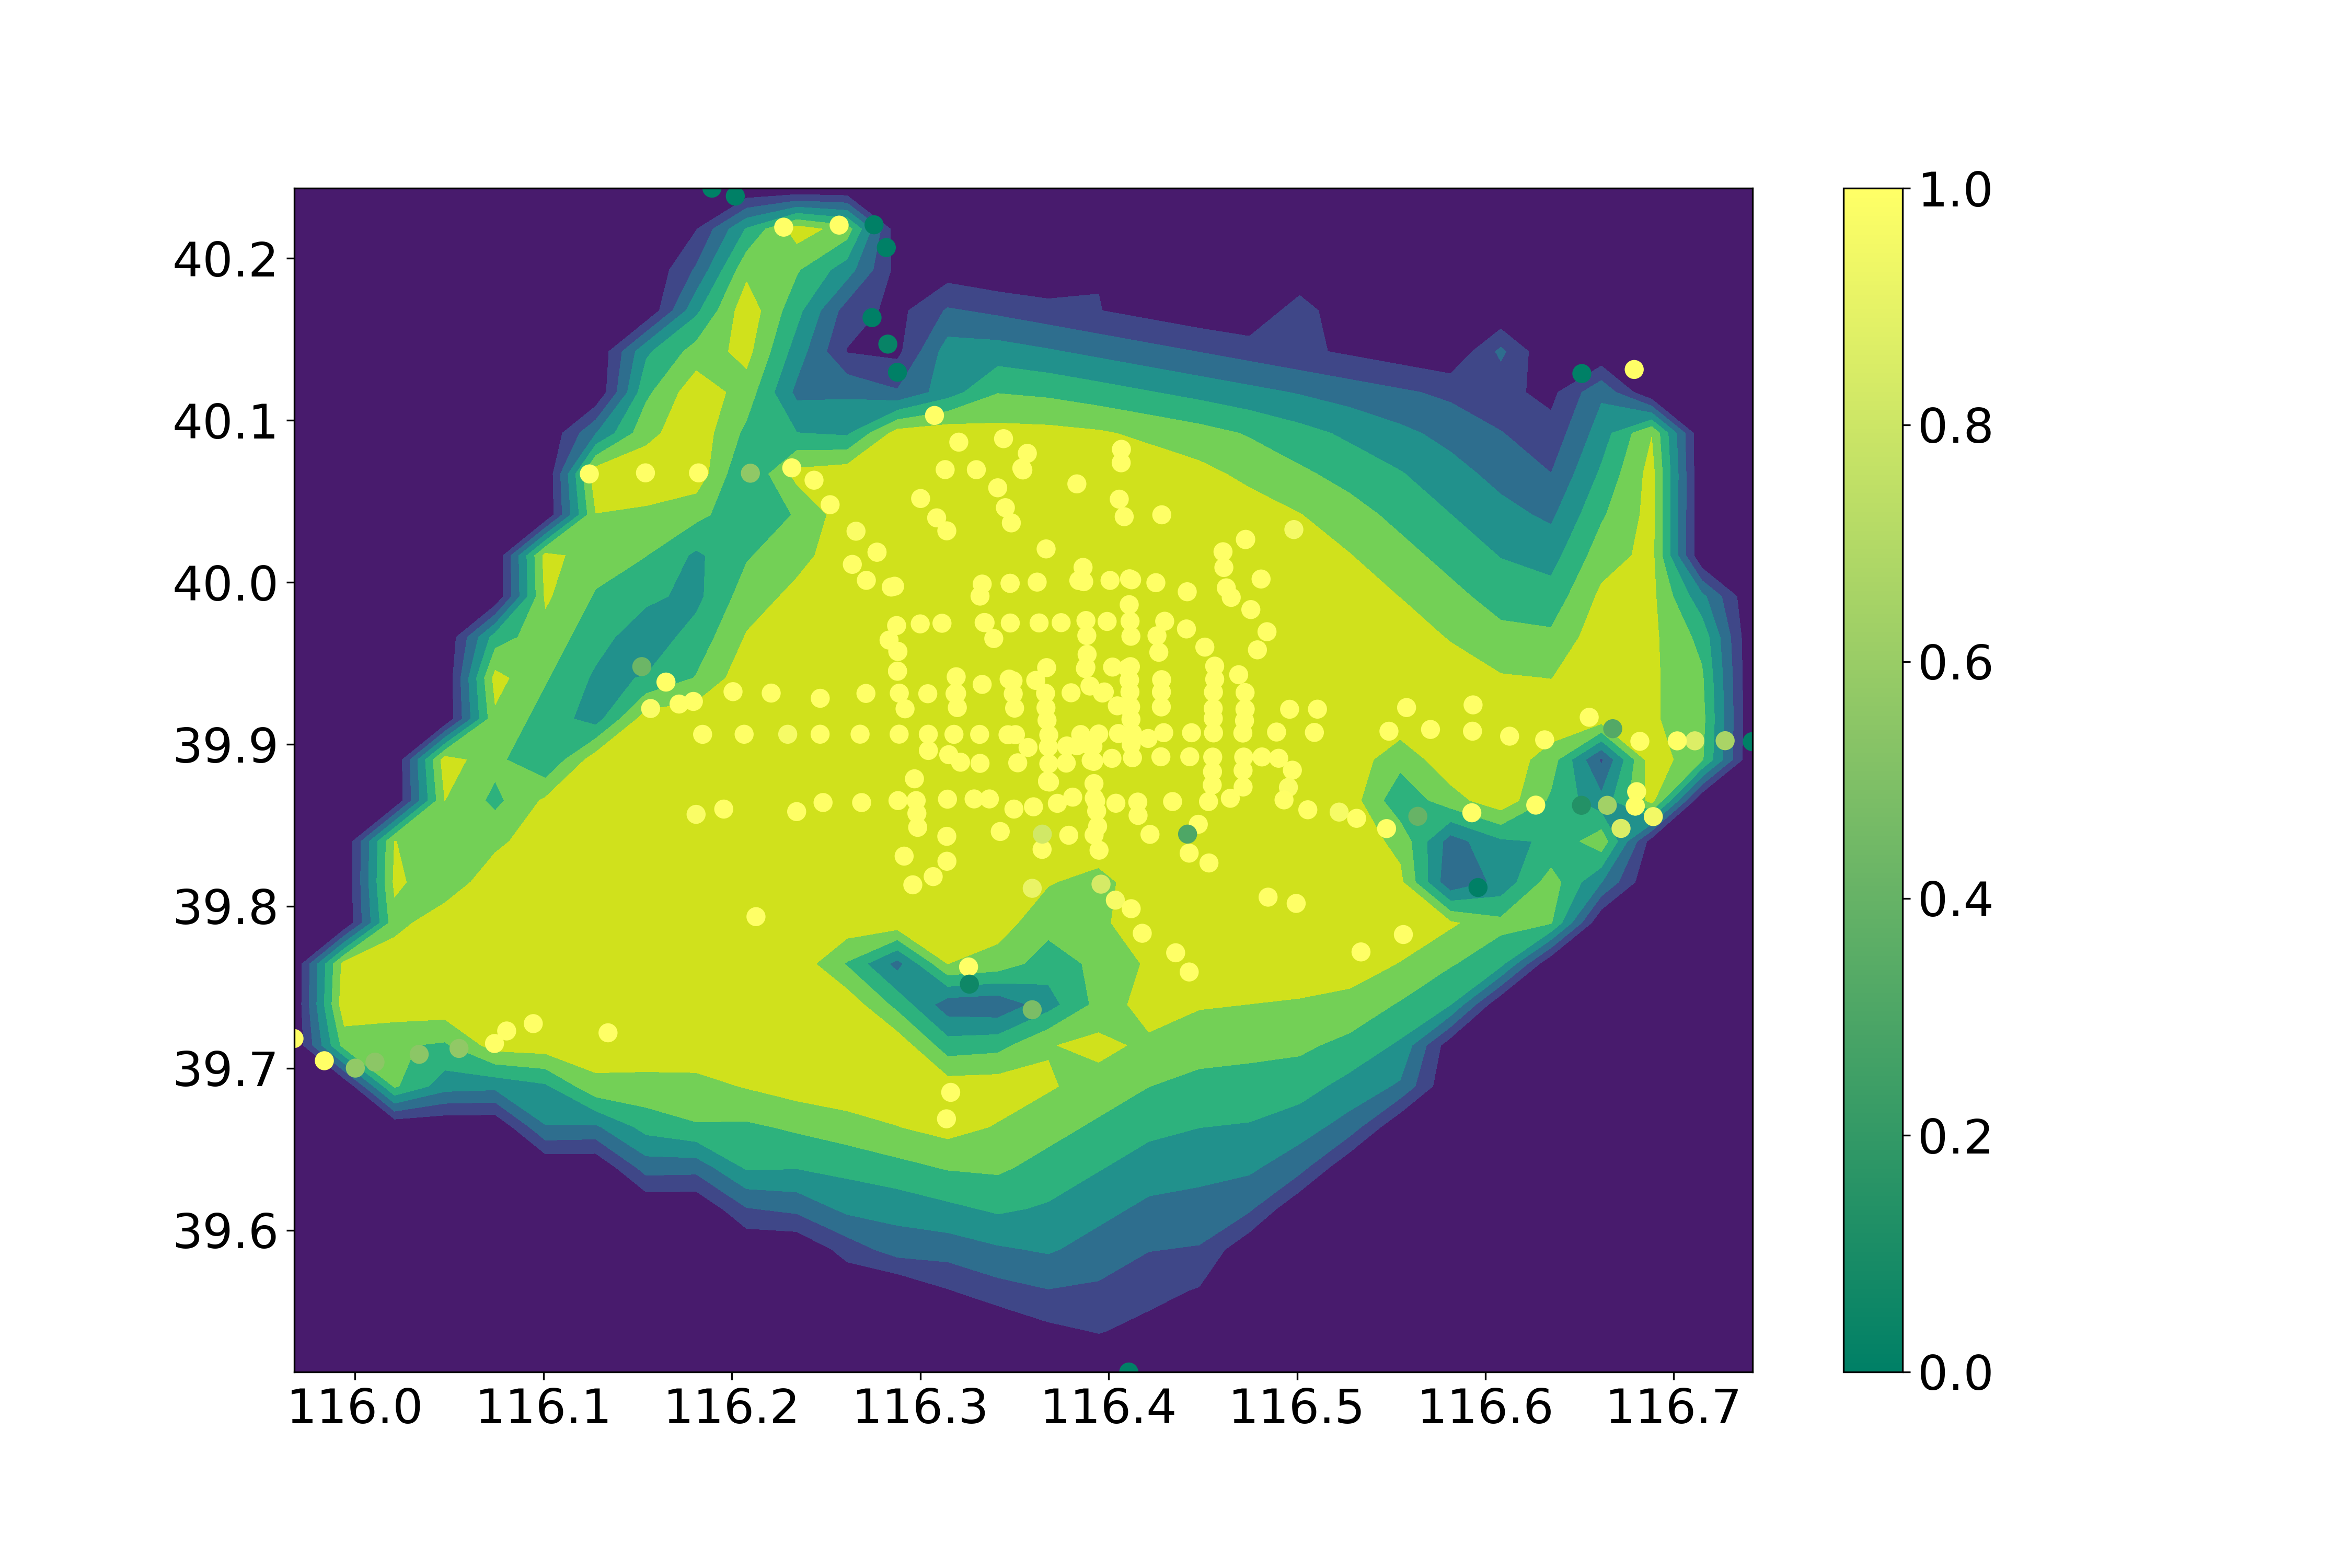
\includegraphics[width=\linewidth]{subway_coverages_0,00333333_lambda_heatmap.png}
		\caption{Mappa di calore ottenuta per $\lambda = 1/300$}
	\end{subfigure}
	\caption[Risultati metropolitana, $\lambda = 1/300$]{I risultati ottenuti applicando il modello alle uscite della metropolitana con $\lambda = 1/300$}
	\label{fig:subway_coverage2}
\end{figure}

\begin{figure}[H]
	\centering
	\begin{subfigure}[b]{\linewidth}
		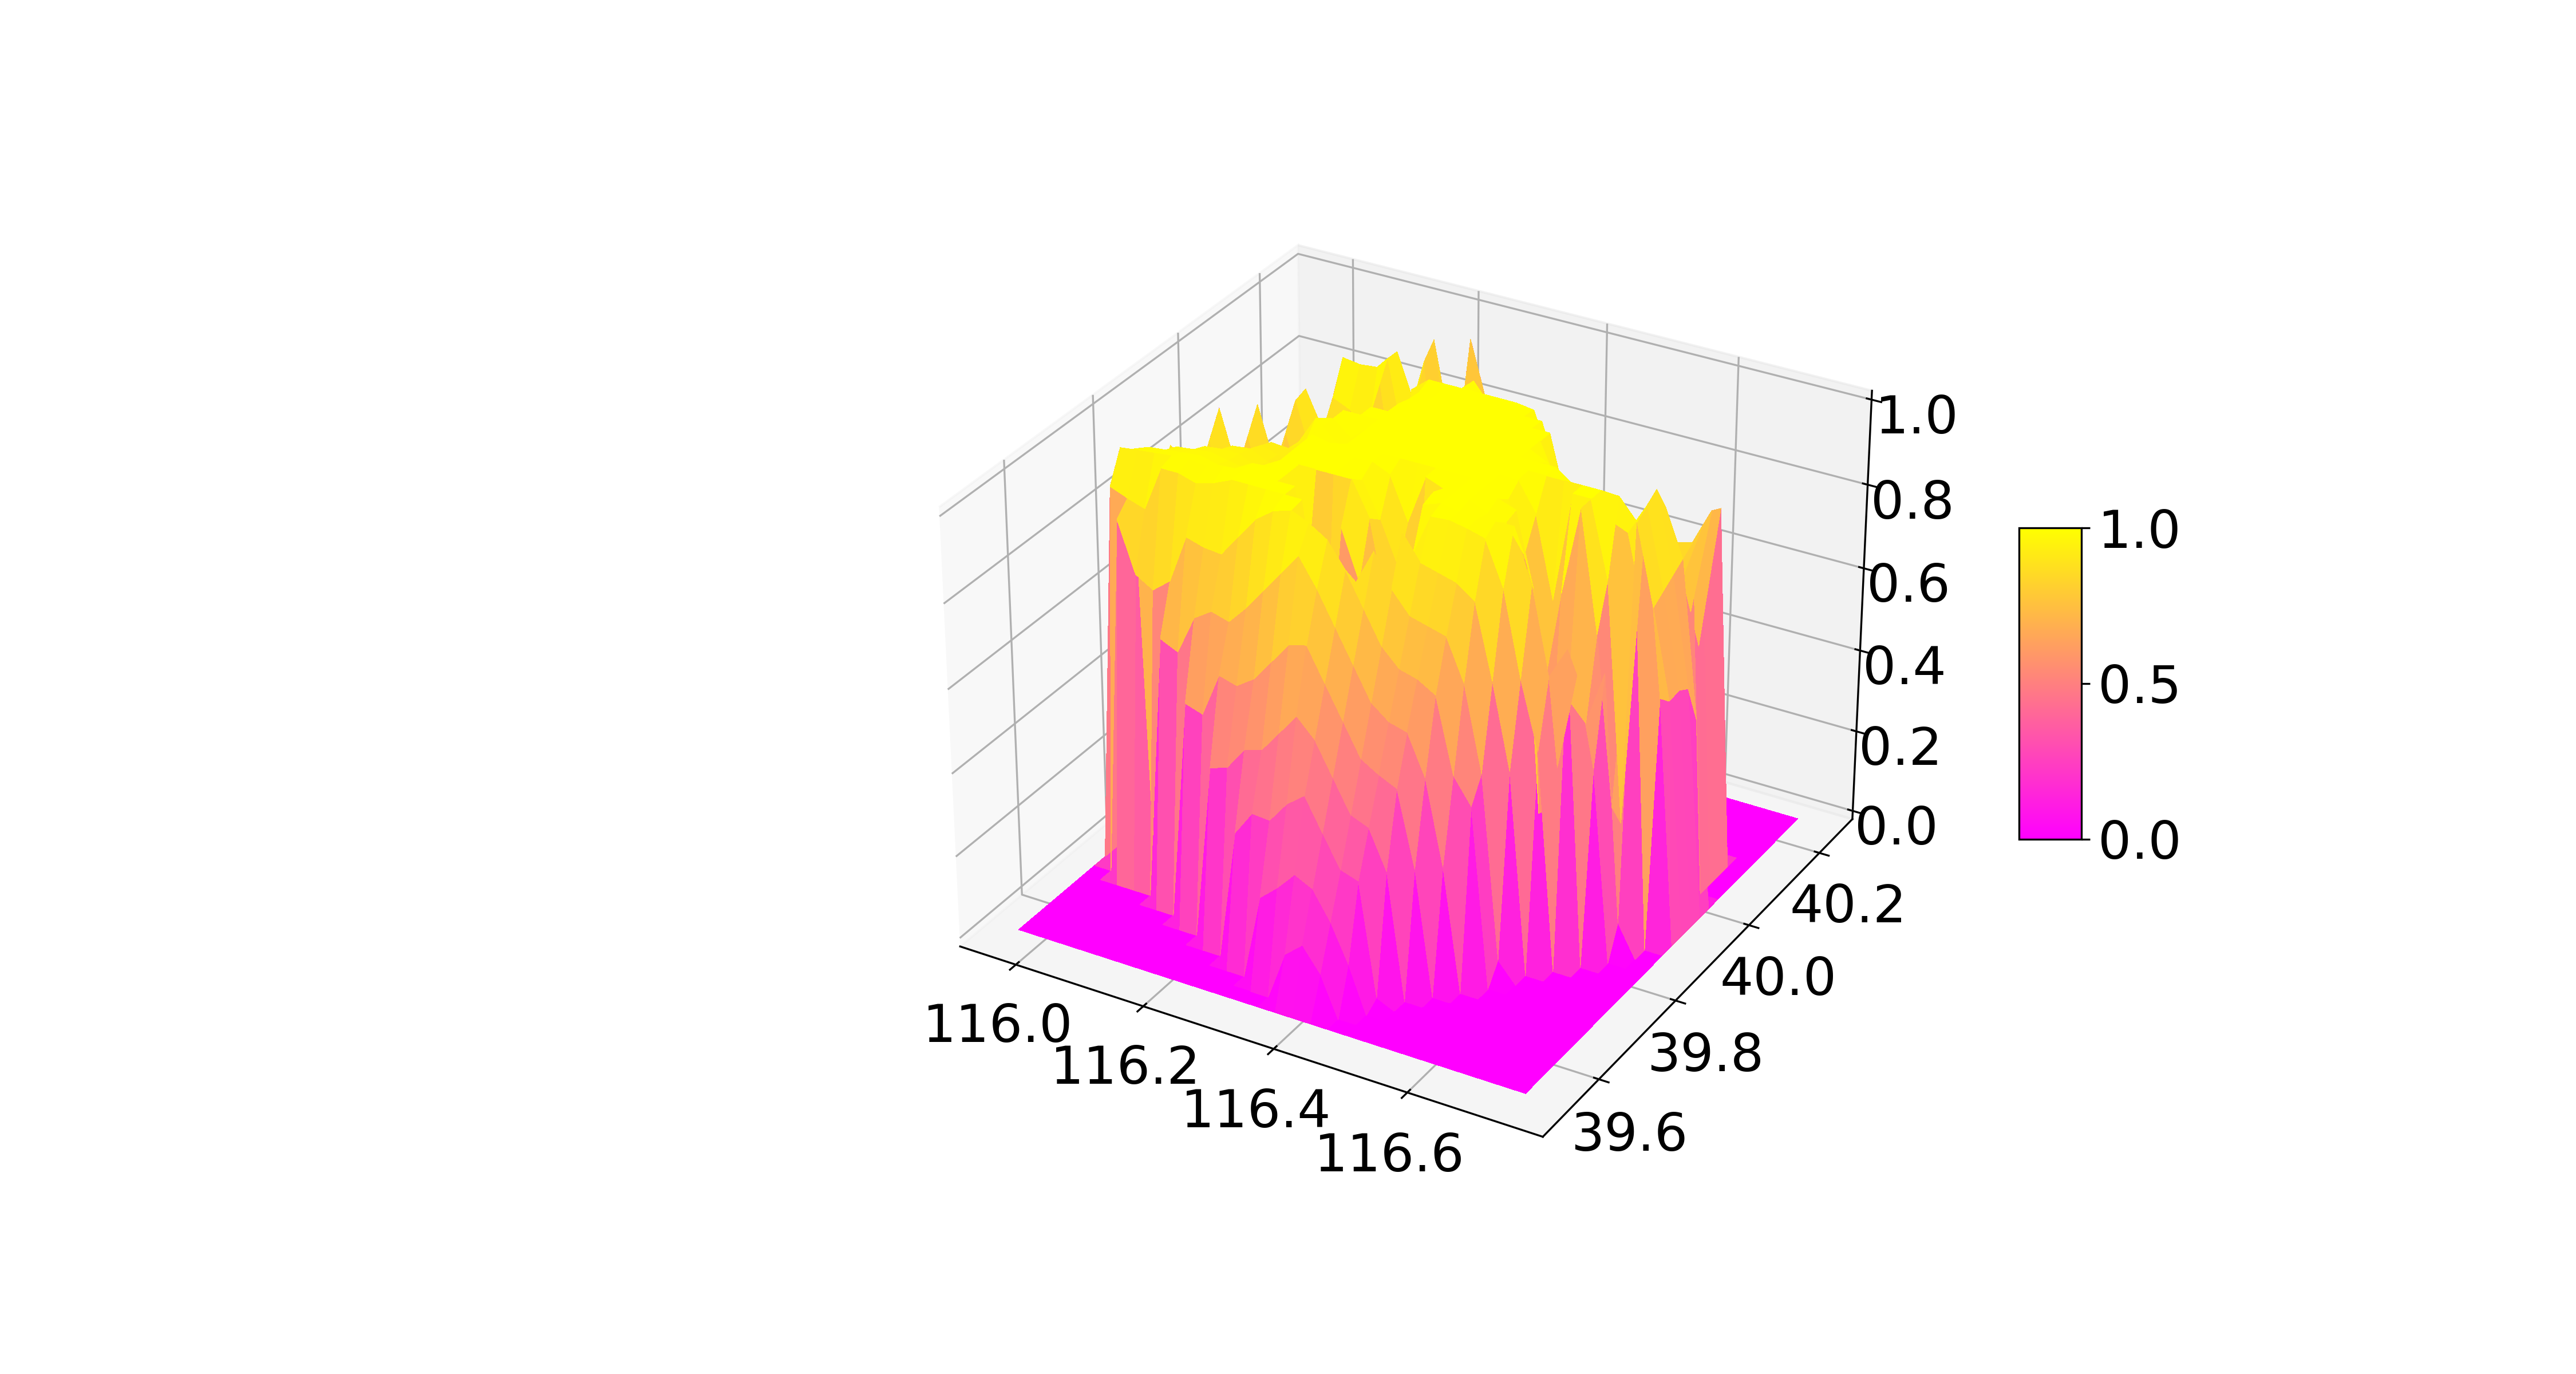
\includegraphics[width=\linewidth]{subway_coverages_0,00142857_lambda_3D_grid.png}
		\caption{Meshgrid ottenuta per $\lambda = 1/700$}
	\end{subfigure}
	\begin{subfigure}[b]{\linewidth}
		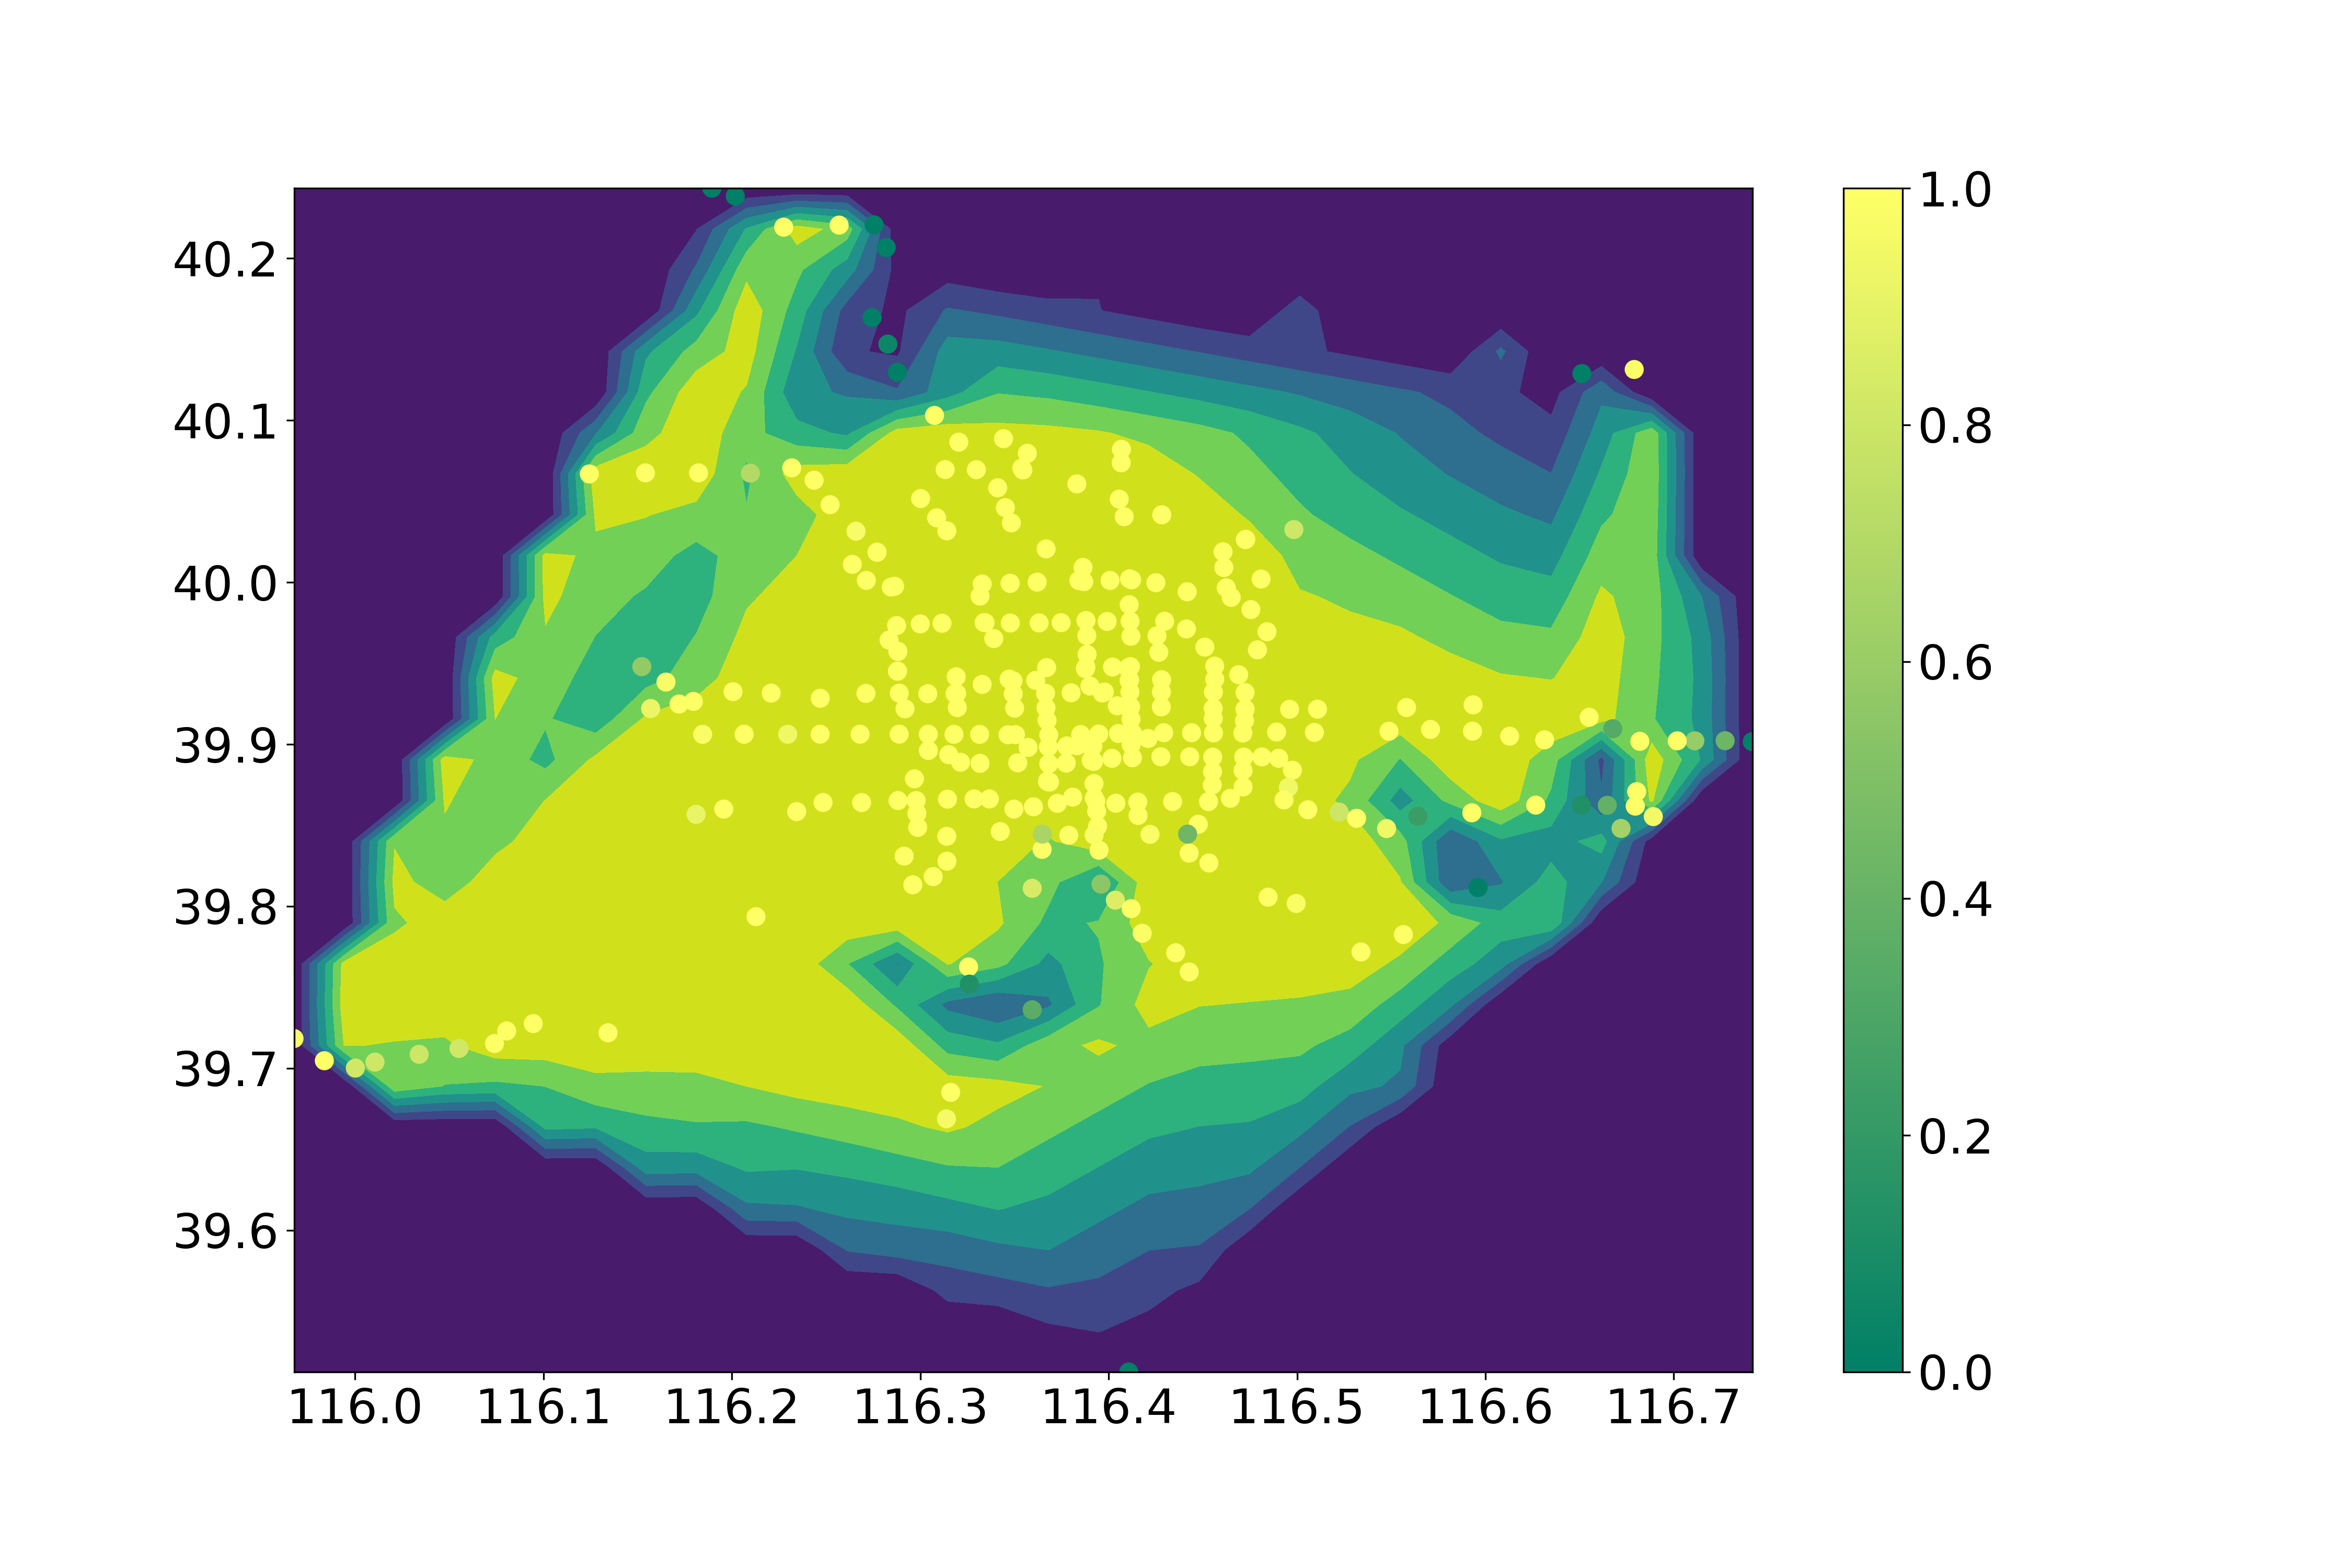
\includegraphics[width=\linewidth]{subway_coverages_0,00142857_lambda_heatmap.png}
		\caption{Mappa di calore ottenuta per $\lambda = 1/700$}
	\end{subfigure}
	\caption[Risultati metropolitana, $\lambda = 1/700$]{I risultati ottenuti applicando il modello alle uscite della metropolitana con $\lambda = 1/700$}
	\label{fig:subway_coverage3}
\end{figure}

\section{Punti di interesse}
I punti di interesse dislocati in tutta la città di Pechino ci permettono di verificare quanto e dove le persone siano più interessate ad andare.
Il data set dei punti di interesse è stato estratto utlizzando OSMnx analogamente a quello delle metropolitane.

Questo tipo di MCS ha un'utilità nel verificare quali siano i luoghi più popolari, e potrebbe essere interessante per studi di tipo turistico e culturale.
\subsection{Punti di interesse considerati
}I punti che sono stati scelti sono tutti monumenti, piazze, edifici storici o luoghi di aggregazione sociale come ad esempio centri commerciali. 
Analogamente a quanto fatto con le uscite della metropolitana, abbiamo estratto le posizioni grazie a OSMnx \cite{osmnx} che permette un filtraggio a grana fine basato su tags per trovare determinate tipologie di punti di interesse.

Dopo la pulizia abbiamo serializzato il dataset, contentente un totale di 956 punti di interesse sparsi in tutta la città.

La Figura \ref{fig:POI} mostra i punti di interesse presi in considerazione, stampati per mezzo di folium \cite{folium}.
Anche in questo caso i cerchi blu rappresentano le singole locazioni e in sovraimpressione sono presenti alcune delle traiettorie di Augmented Geolife.

\begin{figure}[H]
	\centering 
	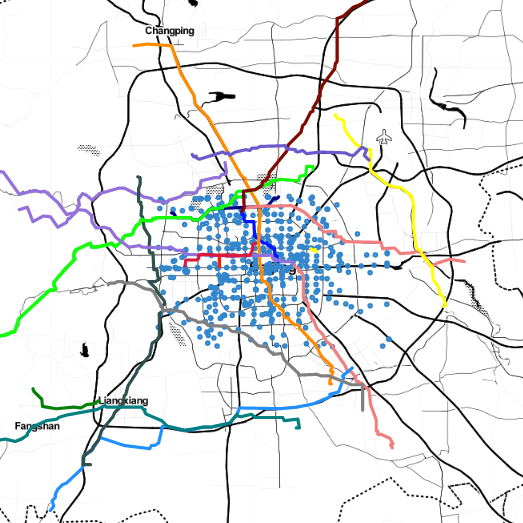
\includegraphics[width=\linewidth]{POI_folium.png}
	\caption[Mappa dei punti di interesse]{I punti di interesse estratti visualizzati grazie a folium}
	\label{fig:POI}
\end{figure}


\subsection{Risultati del modello di coverage}
Le Figure \ref{fig:POIs_coverage1}, \ref{fig:POIs_coverage2}, e \ref{fig:POIs_coverage3}, mostrano i risultati ottenuti applicando il modello con differenti valori di lambda sui punti di interesse estratti per mezzo di OSMnx \cite{osmnx}. 

\newpage

\begin{figure}[H]
	\centering
	\begin{subfigure}[b]{\linewidth}
		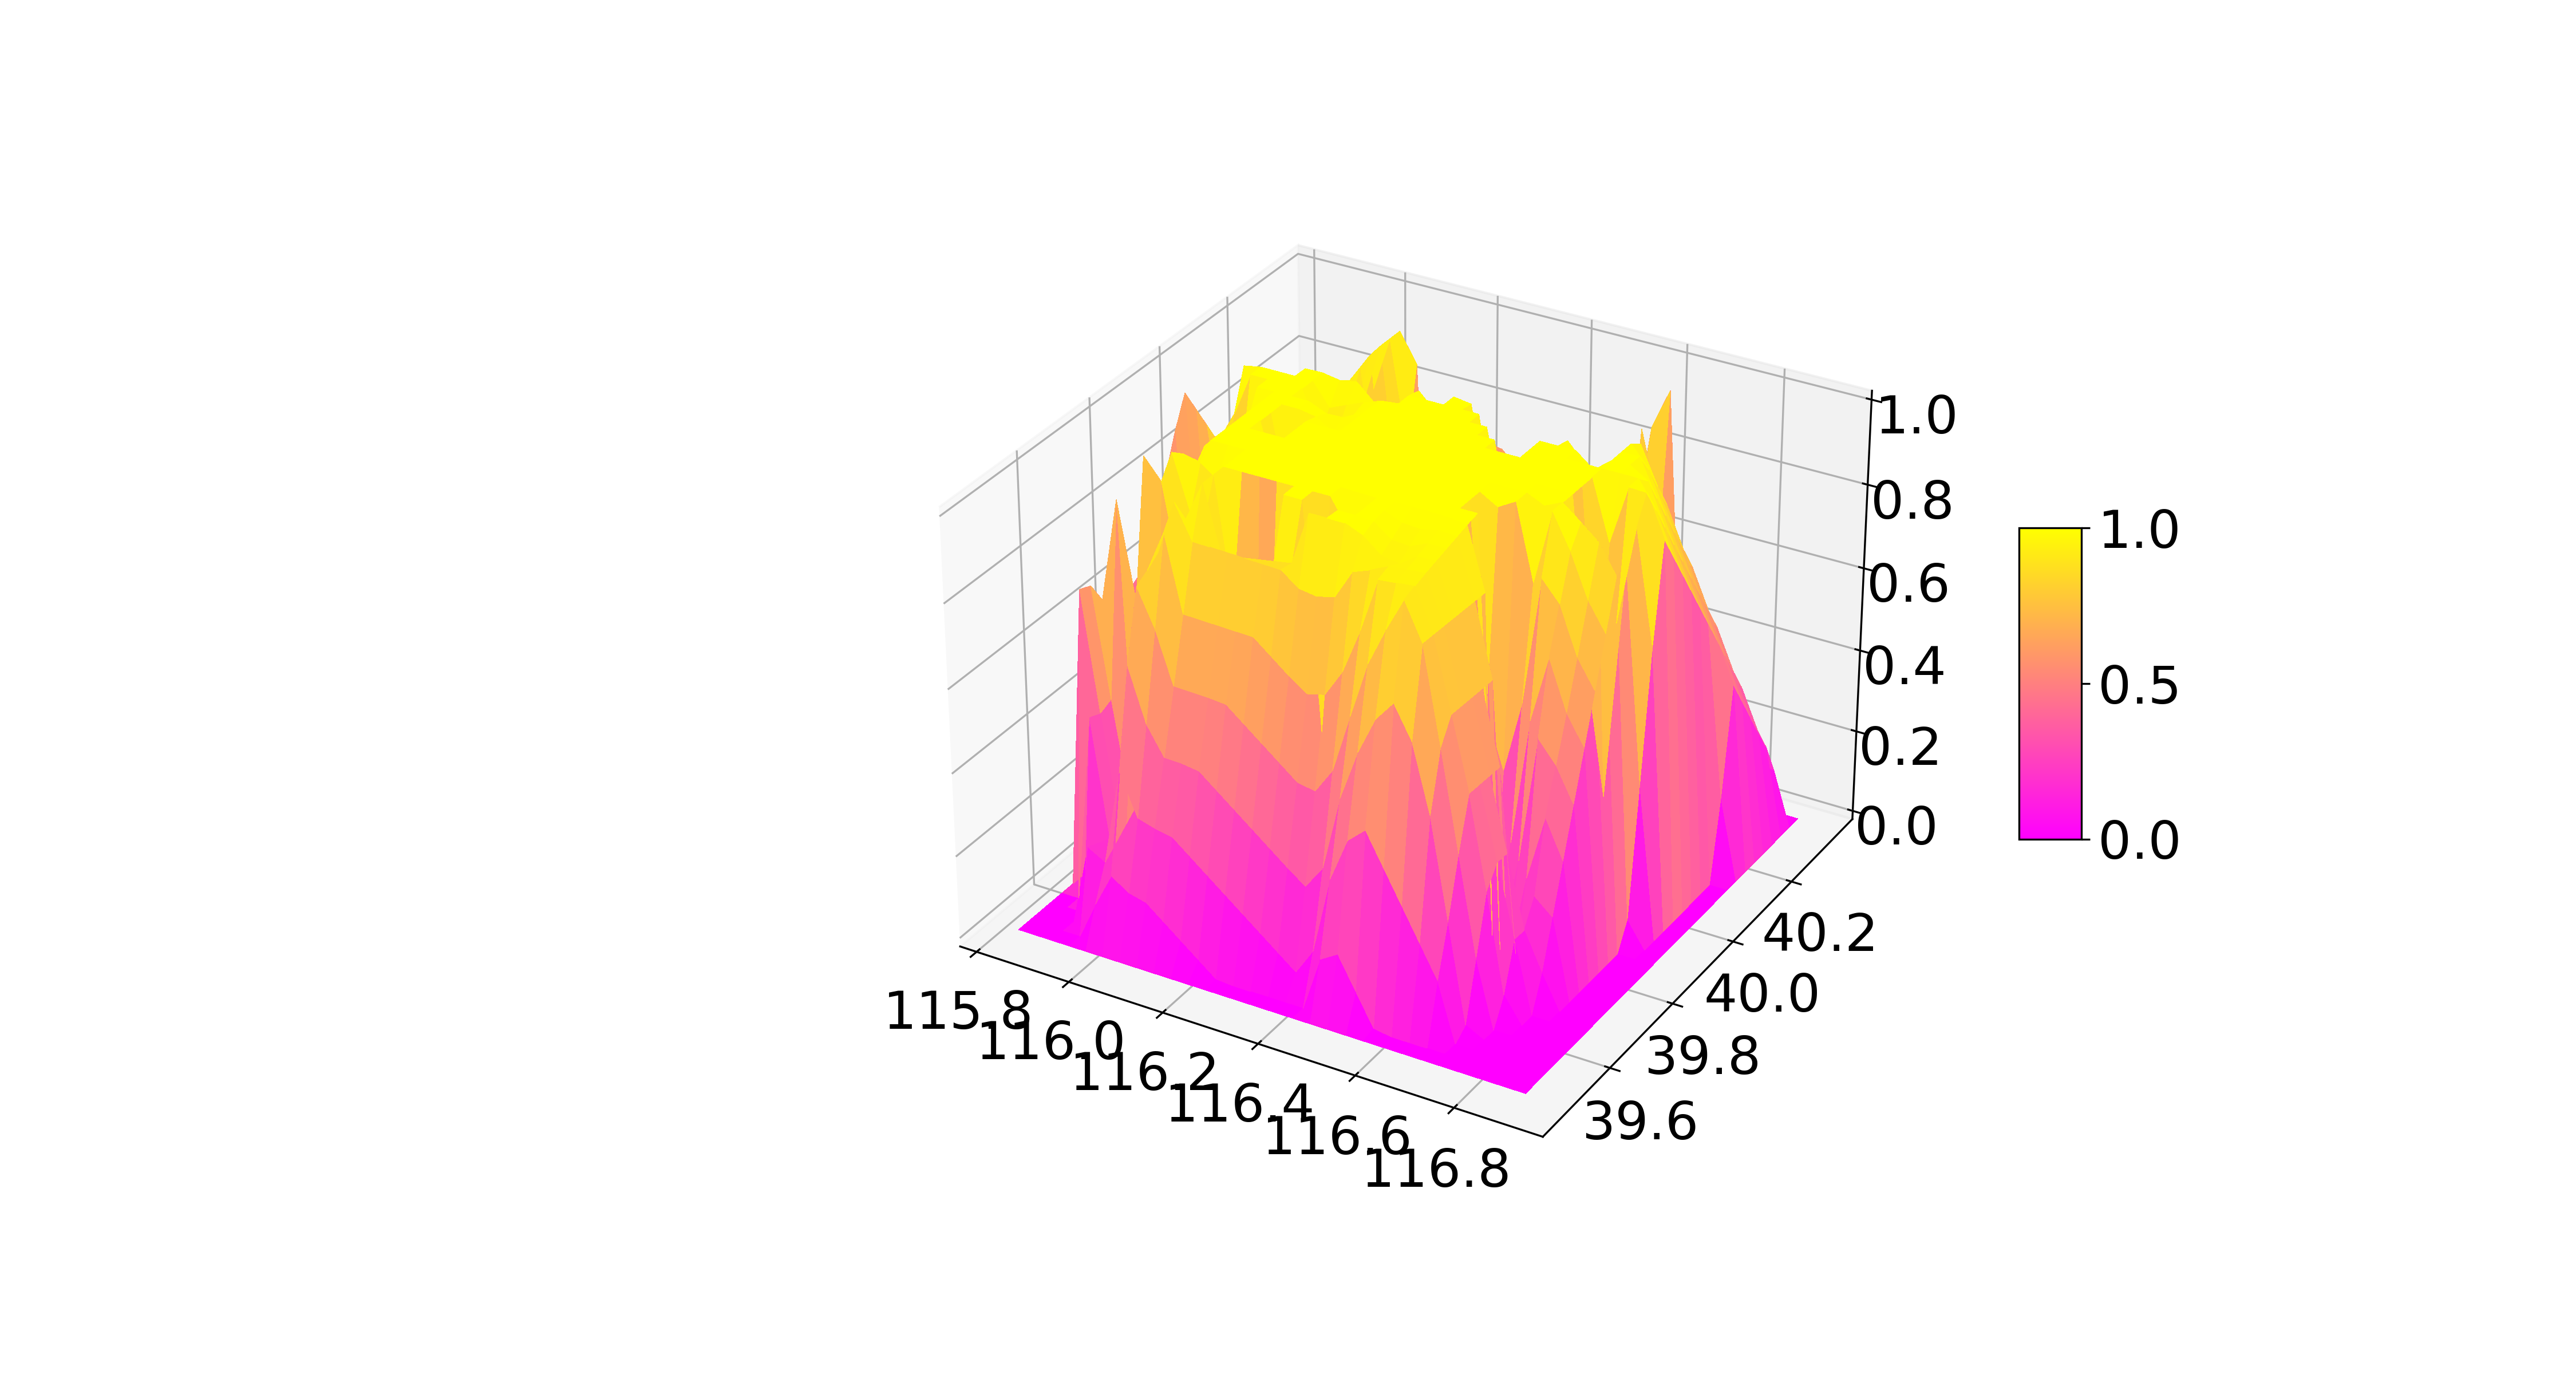
\includegraphics[width=\linewidth]{POIs_coverages_0,01_lambda_3D_grid.png}
		\caption{Meshgrid ottenuta per $\lambda = 1/100$}
	\end{subfigure}
	\begin{subfigure}[b]{\linewidth}
		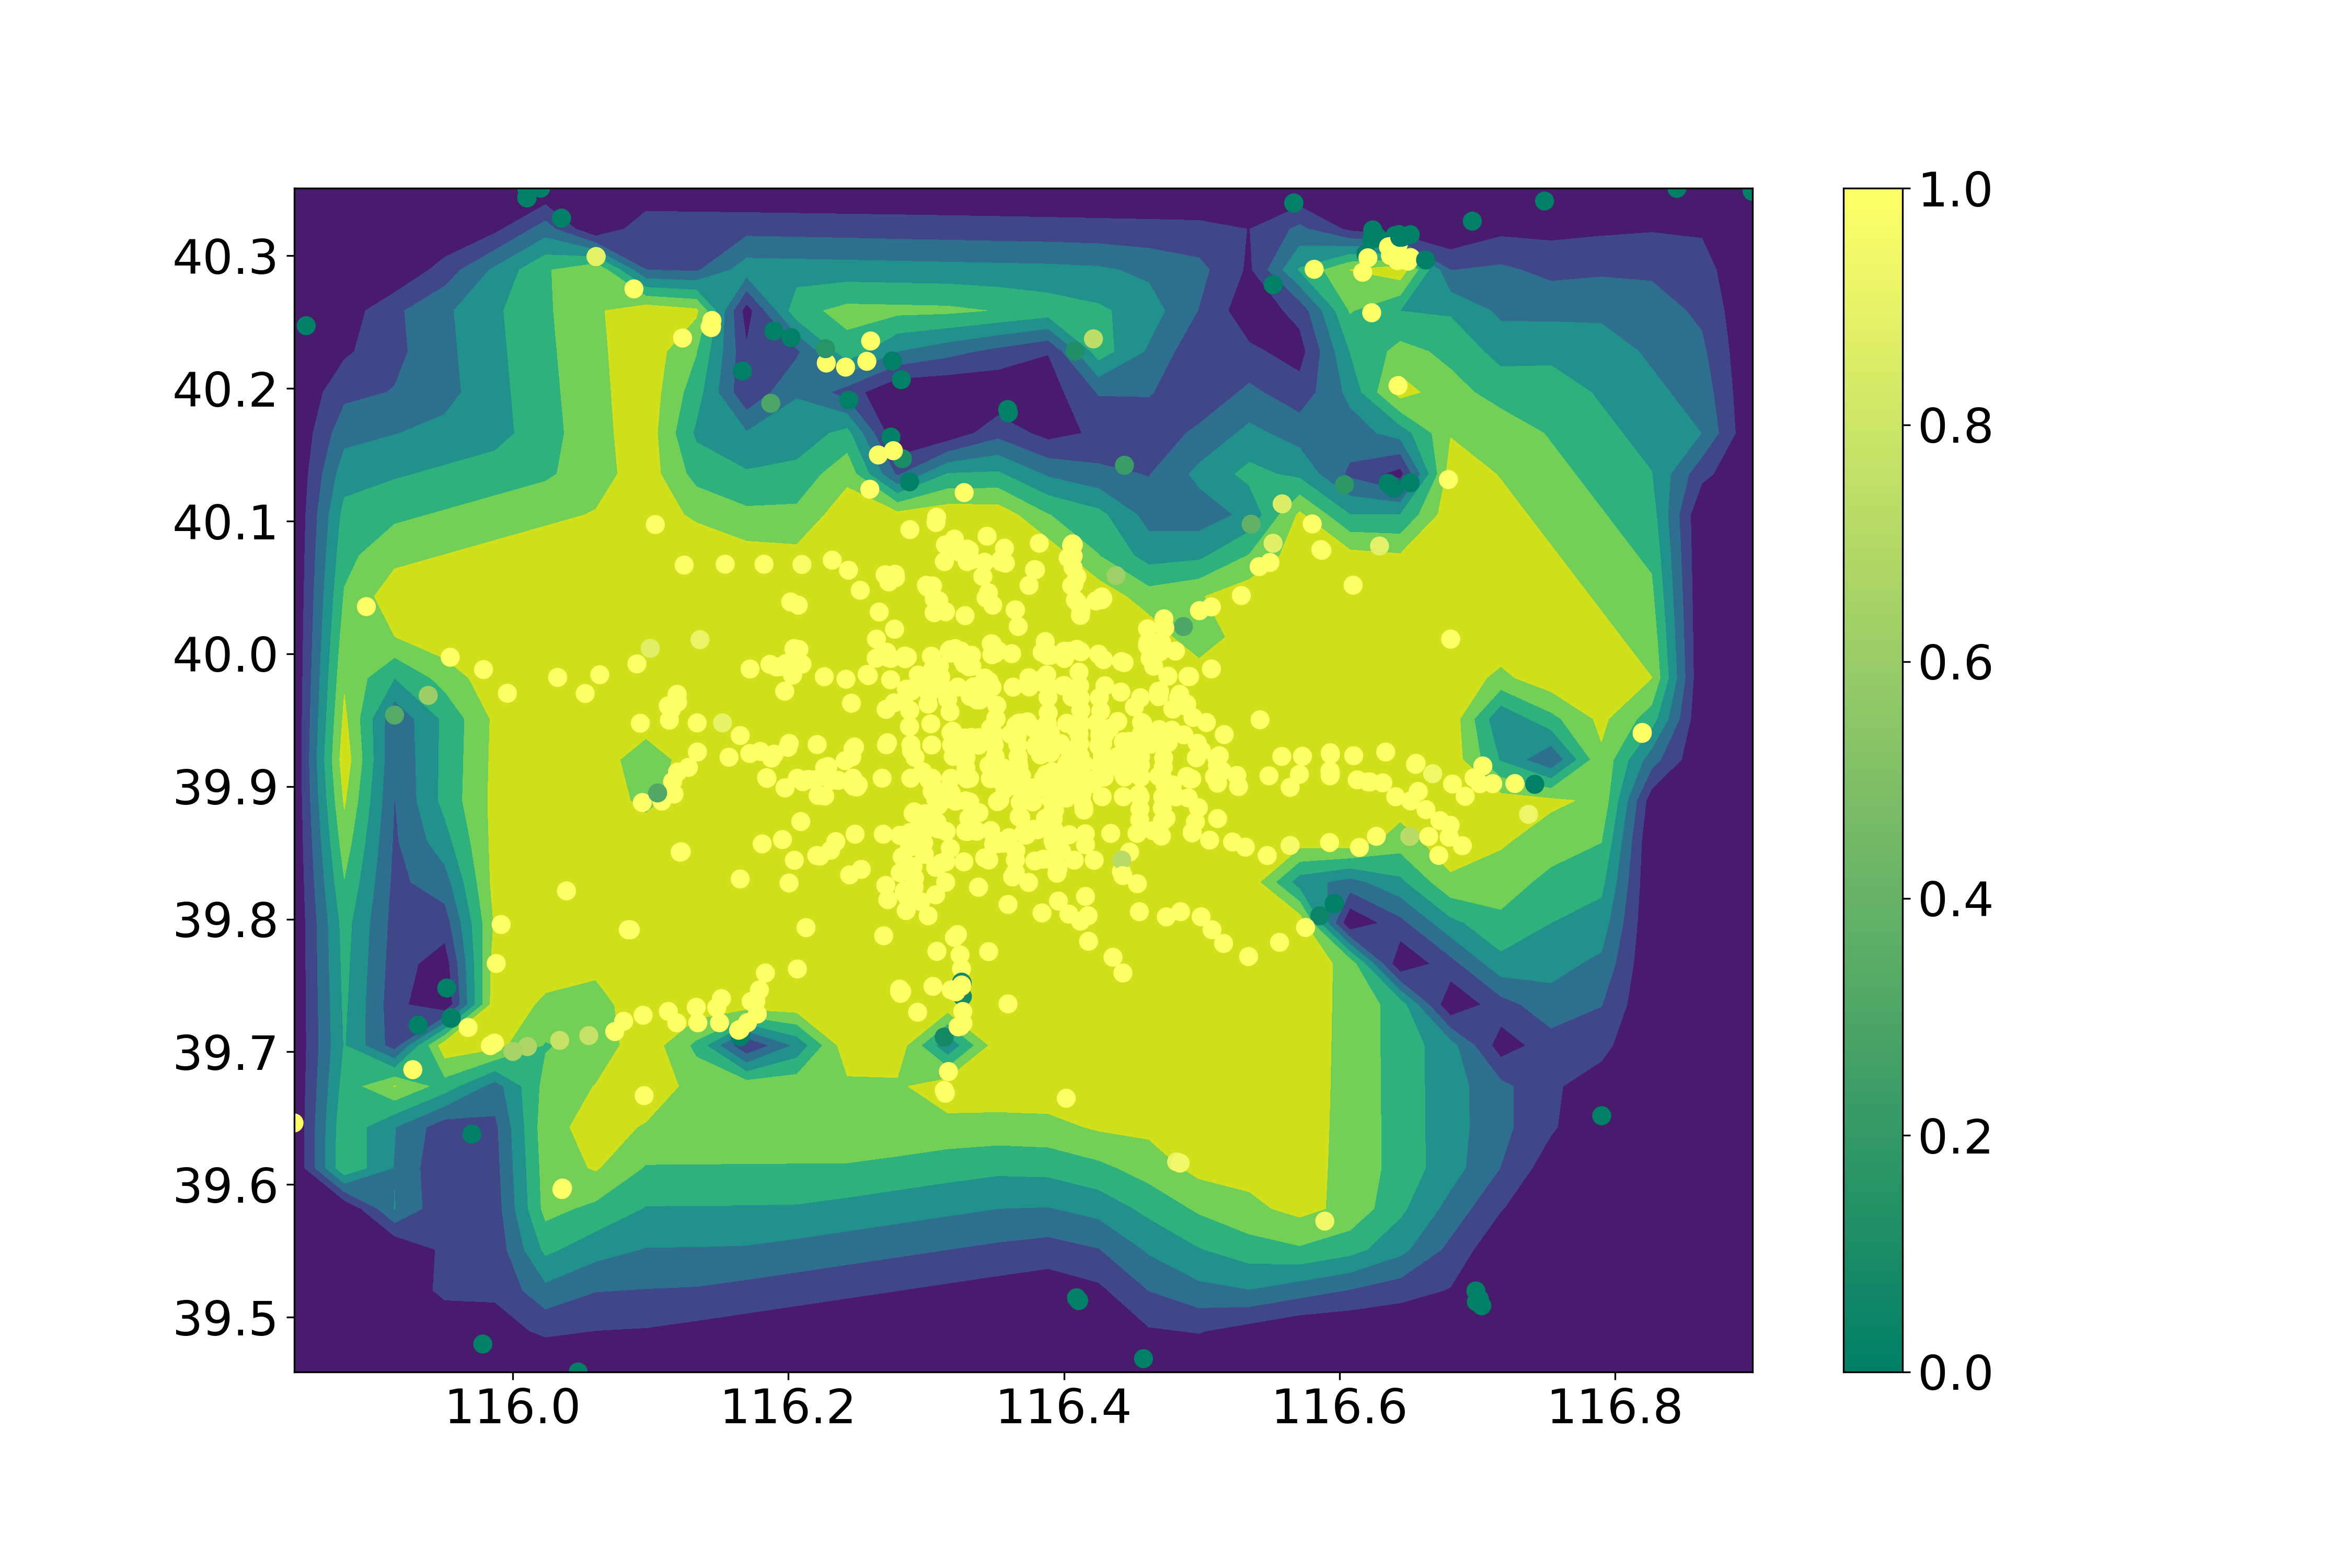
\includegraphics[width=\linewidth]{POIs_coverages_0,01_lambda_heatmap.png}
		\caption{Mappa di calore ottenuta per $\lambda = 1/100$}
	\end{subfigure}
	\caption[Risultati POIs, $\lambda = 1/100$]{I risultati ottenuti applicando il modello ai punti di interesse con $\lambda = 1/100$}
	\label{fig:POIs_coverage1}
\end{figure}

\begin{figure}[H]
	\centering
	\begin{subfigure}[b]{\linewidth}
		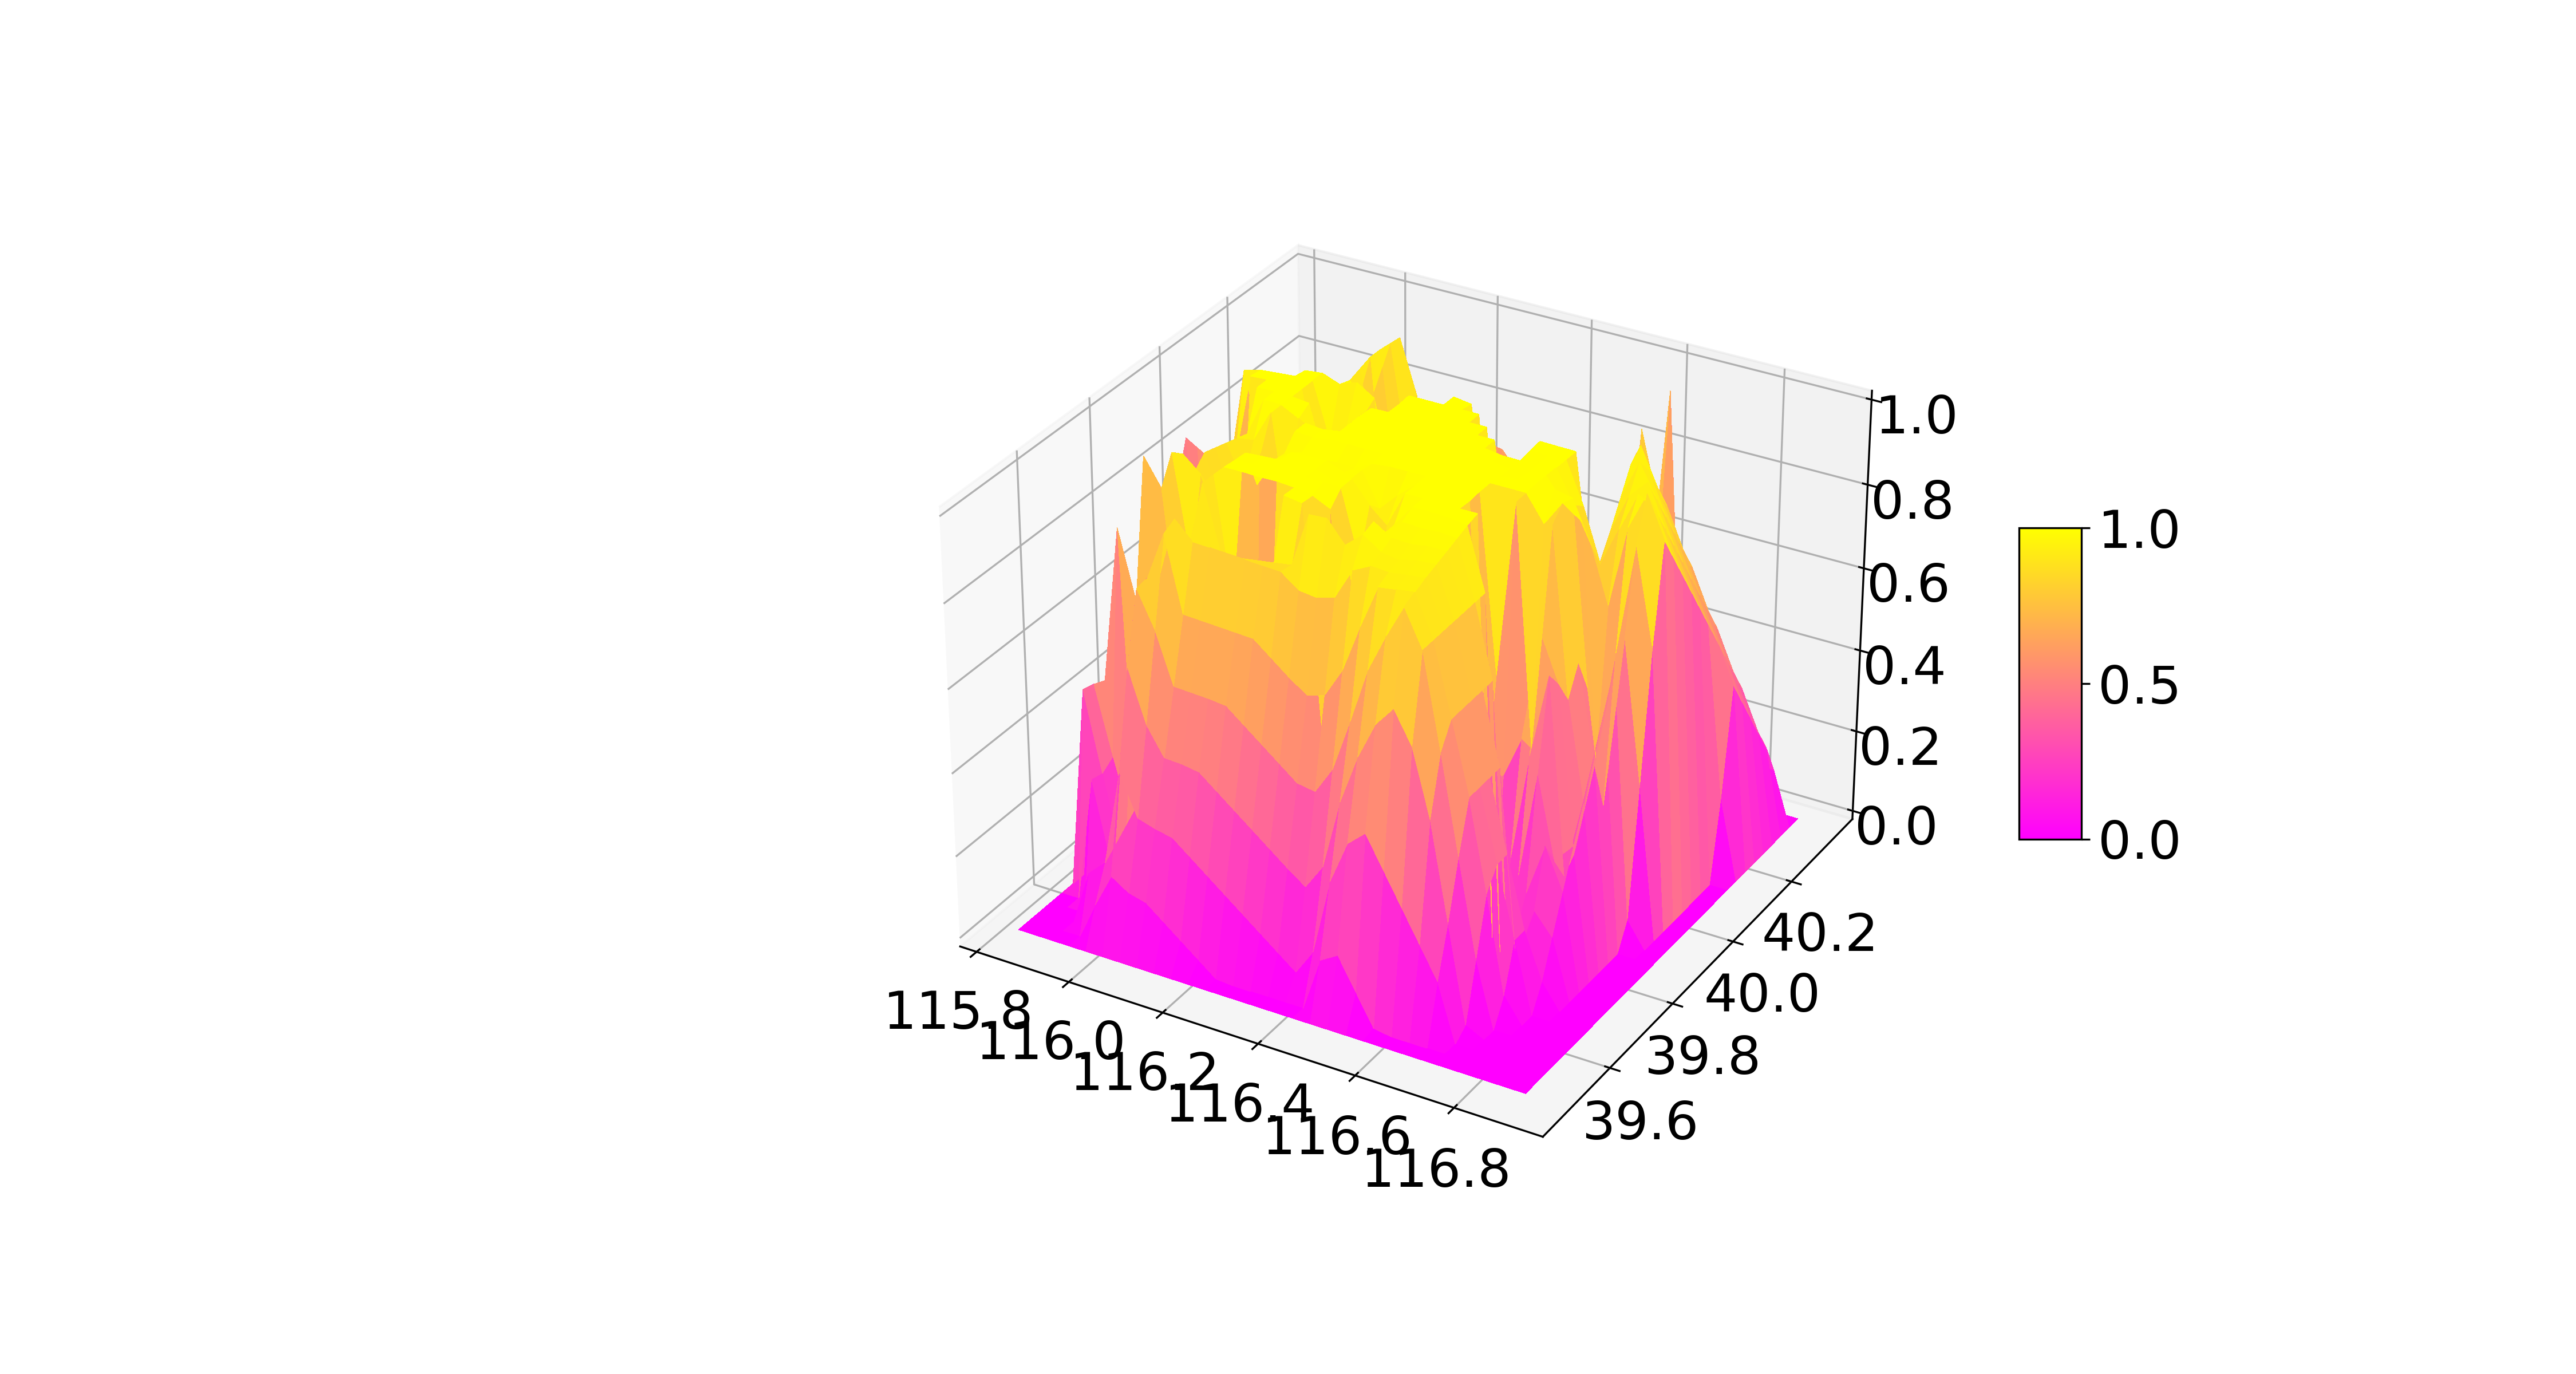
\includegraphics[width=\linewidth]{POIs_coverages_0,00333333_lambda_3D_grid.png}
		\caption{Meshgrid ottenuta per $\lambda = 1/300$}
	\end{subfigure}
	\begin{subfigure}[b]{\linewidth}
		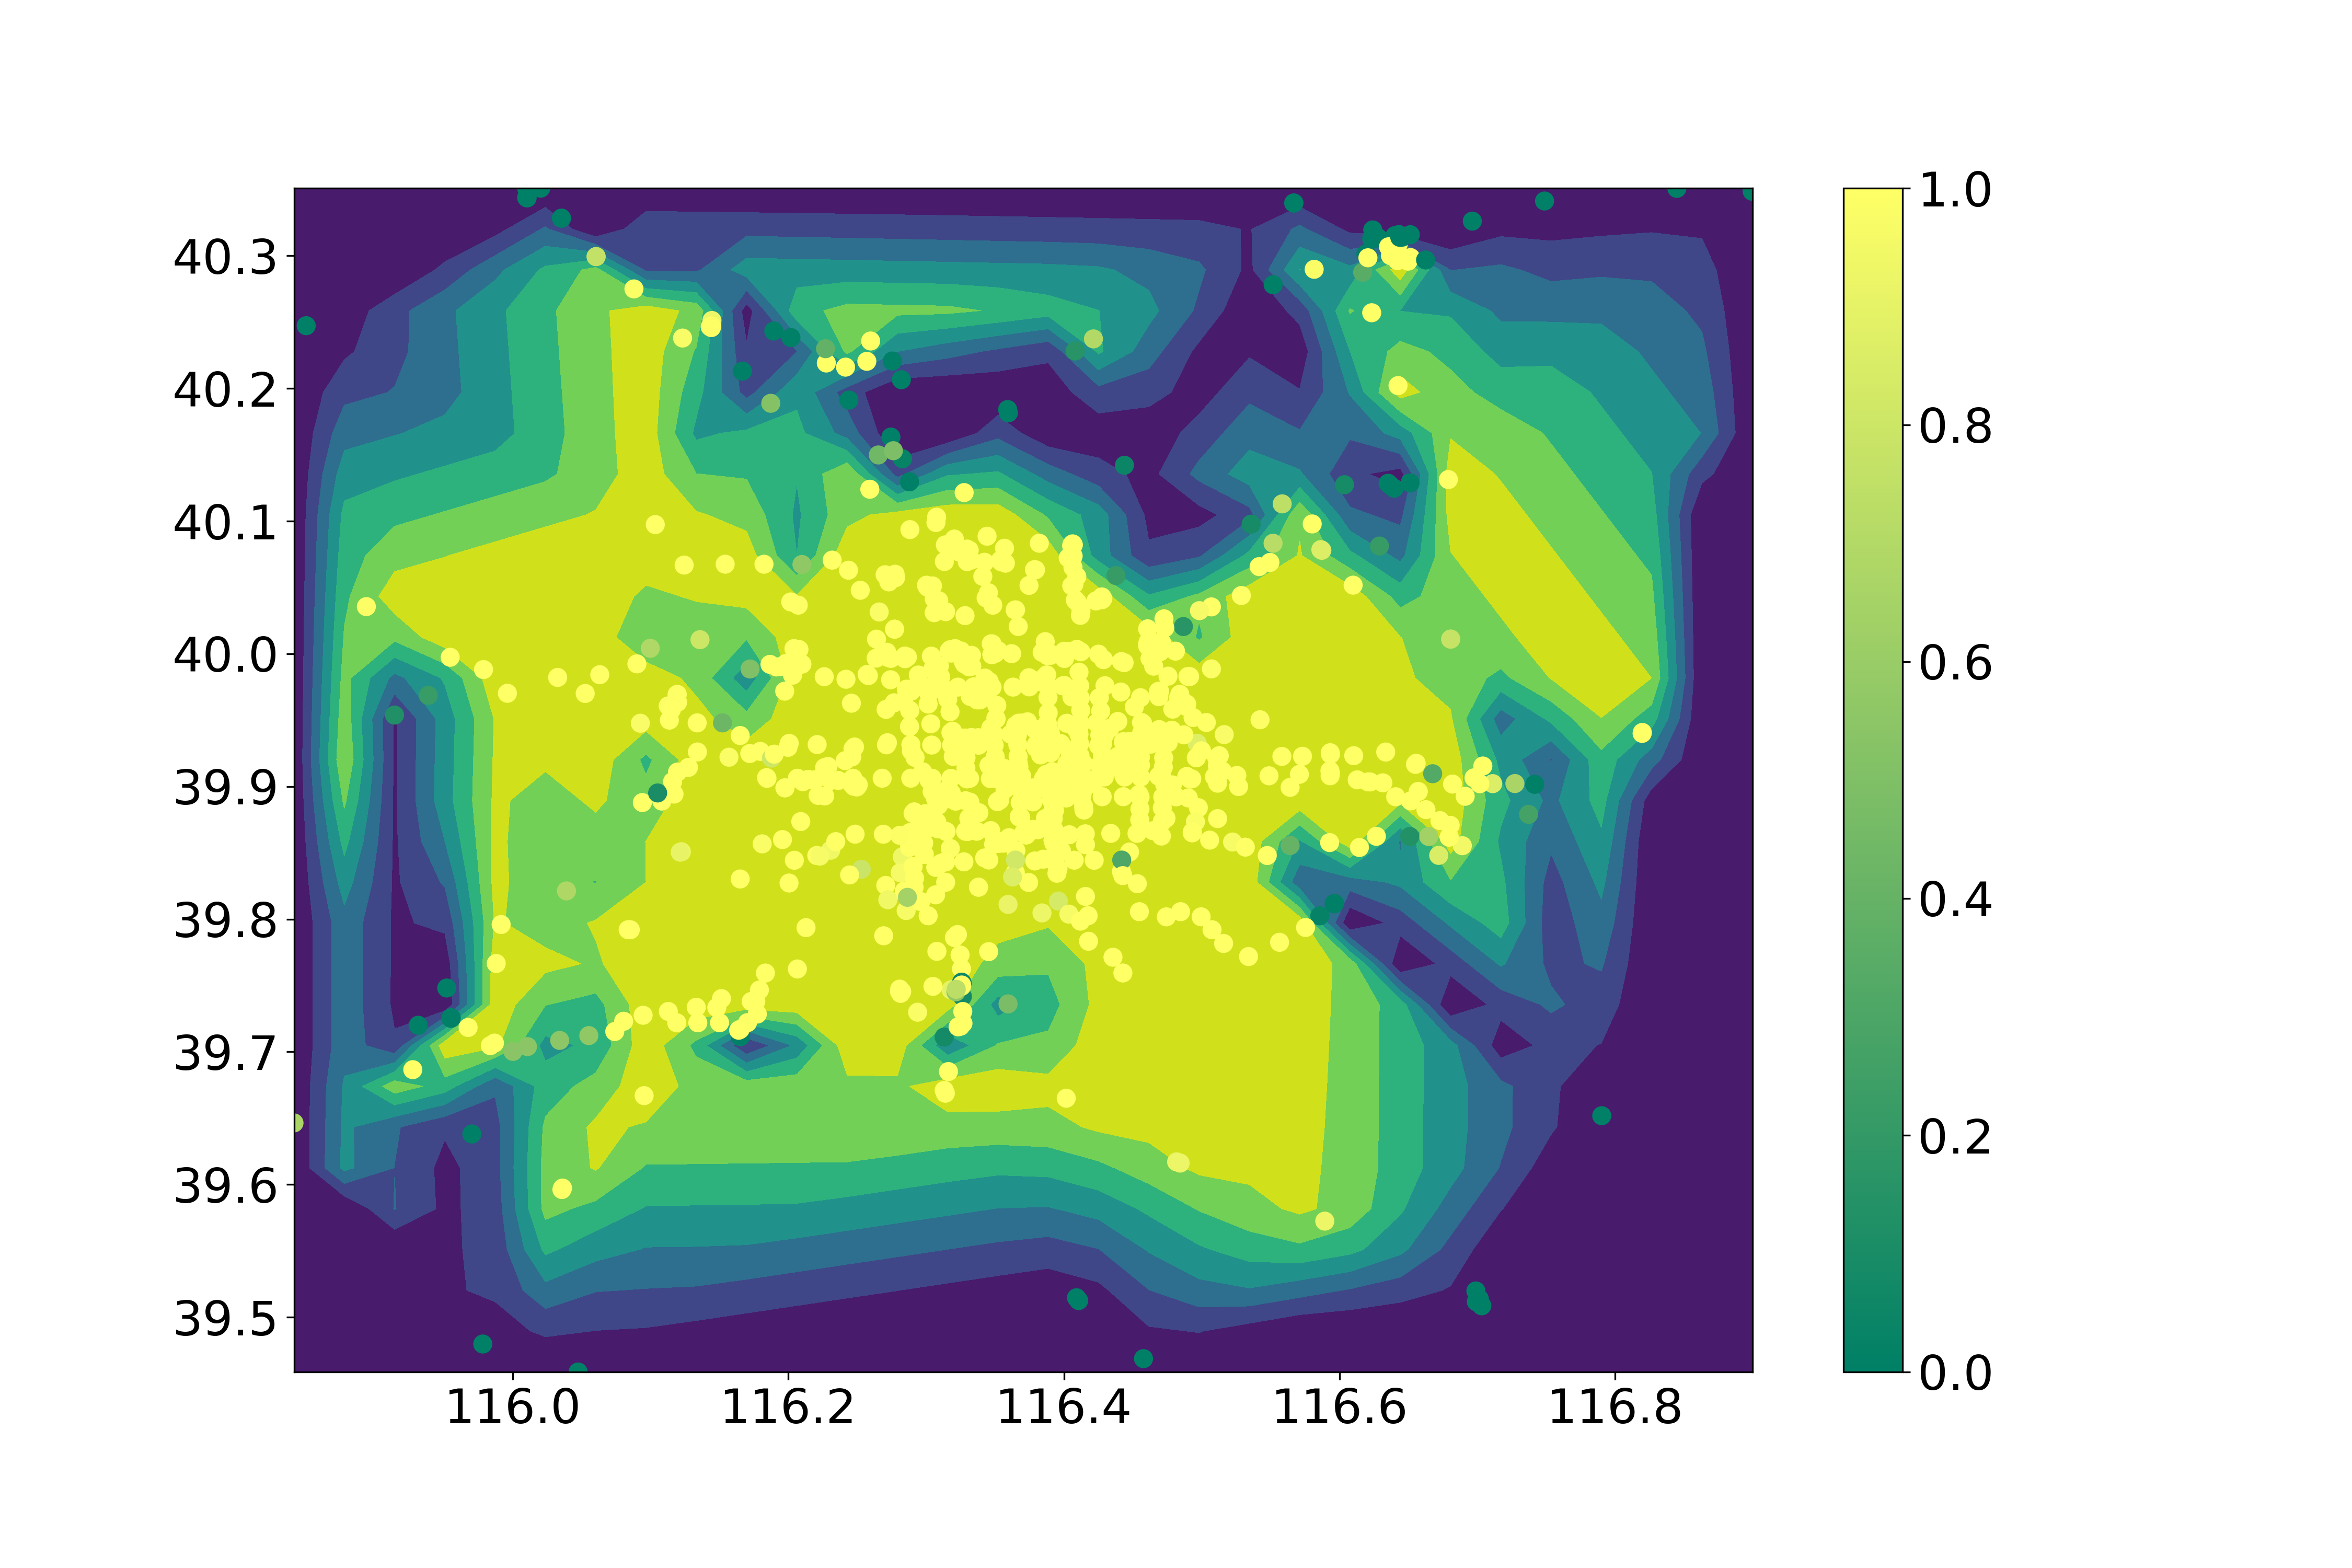
\includegraphics[width=\linewidth]{POIs_coverages_0,00333333_lambda_heatmap.png}
		\caption{Mappa di calore ottenuta per $\lambda = 1/300$}
	\end{subfigure}
	\caption[Risultati POIs, $\lambda = 1/300$]{I risultati ottenuti applicando il modello ai punti di interesse con $\lambda = 1/300$}
	\label{fig:POIs_coverage2}
\end{figure}

\begin{figure}[H]
	\centering
	\begin{subfigure}[b]{\linewidth}
		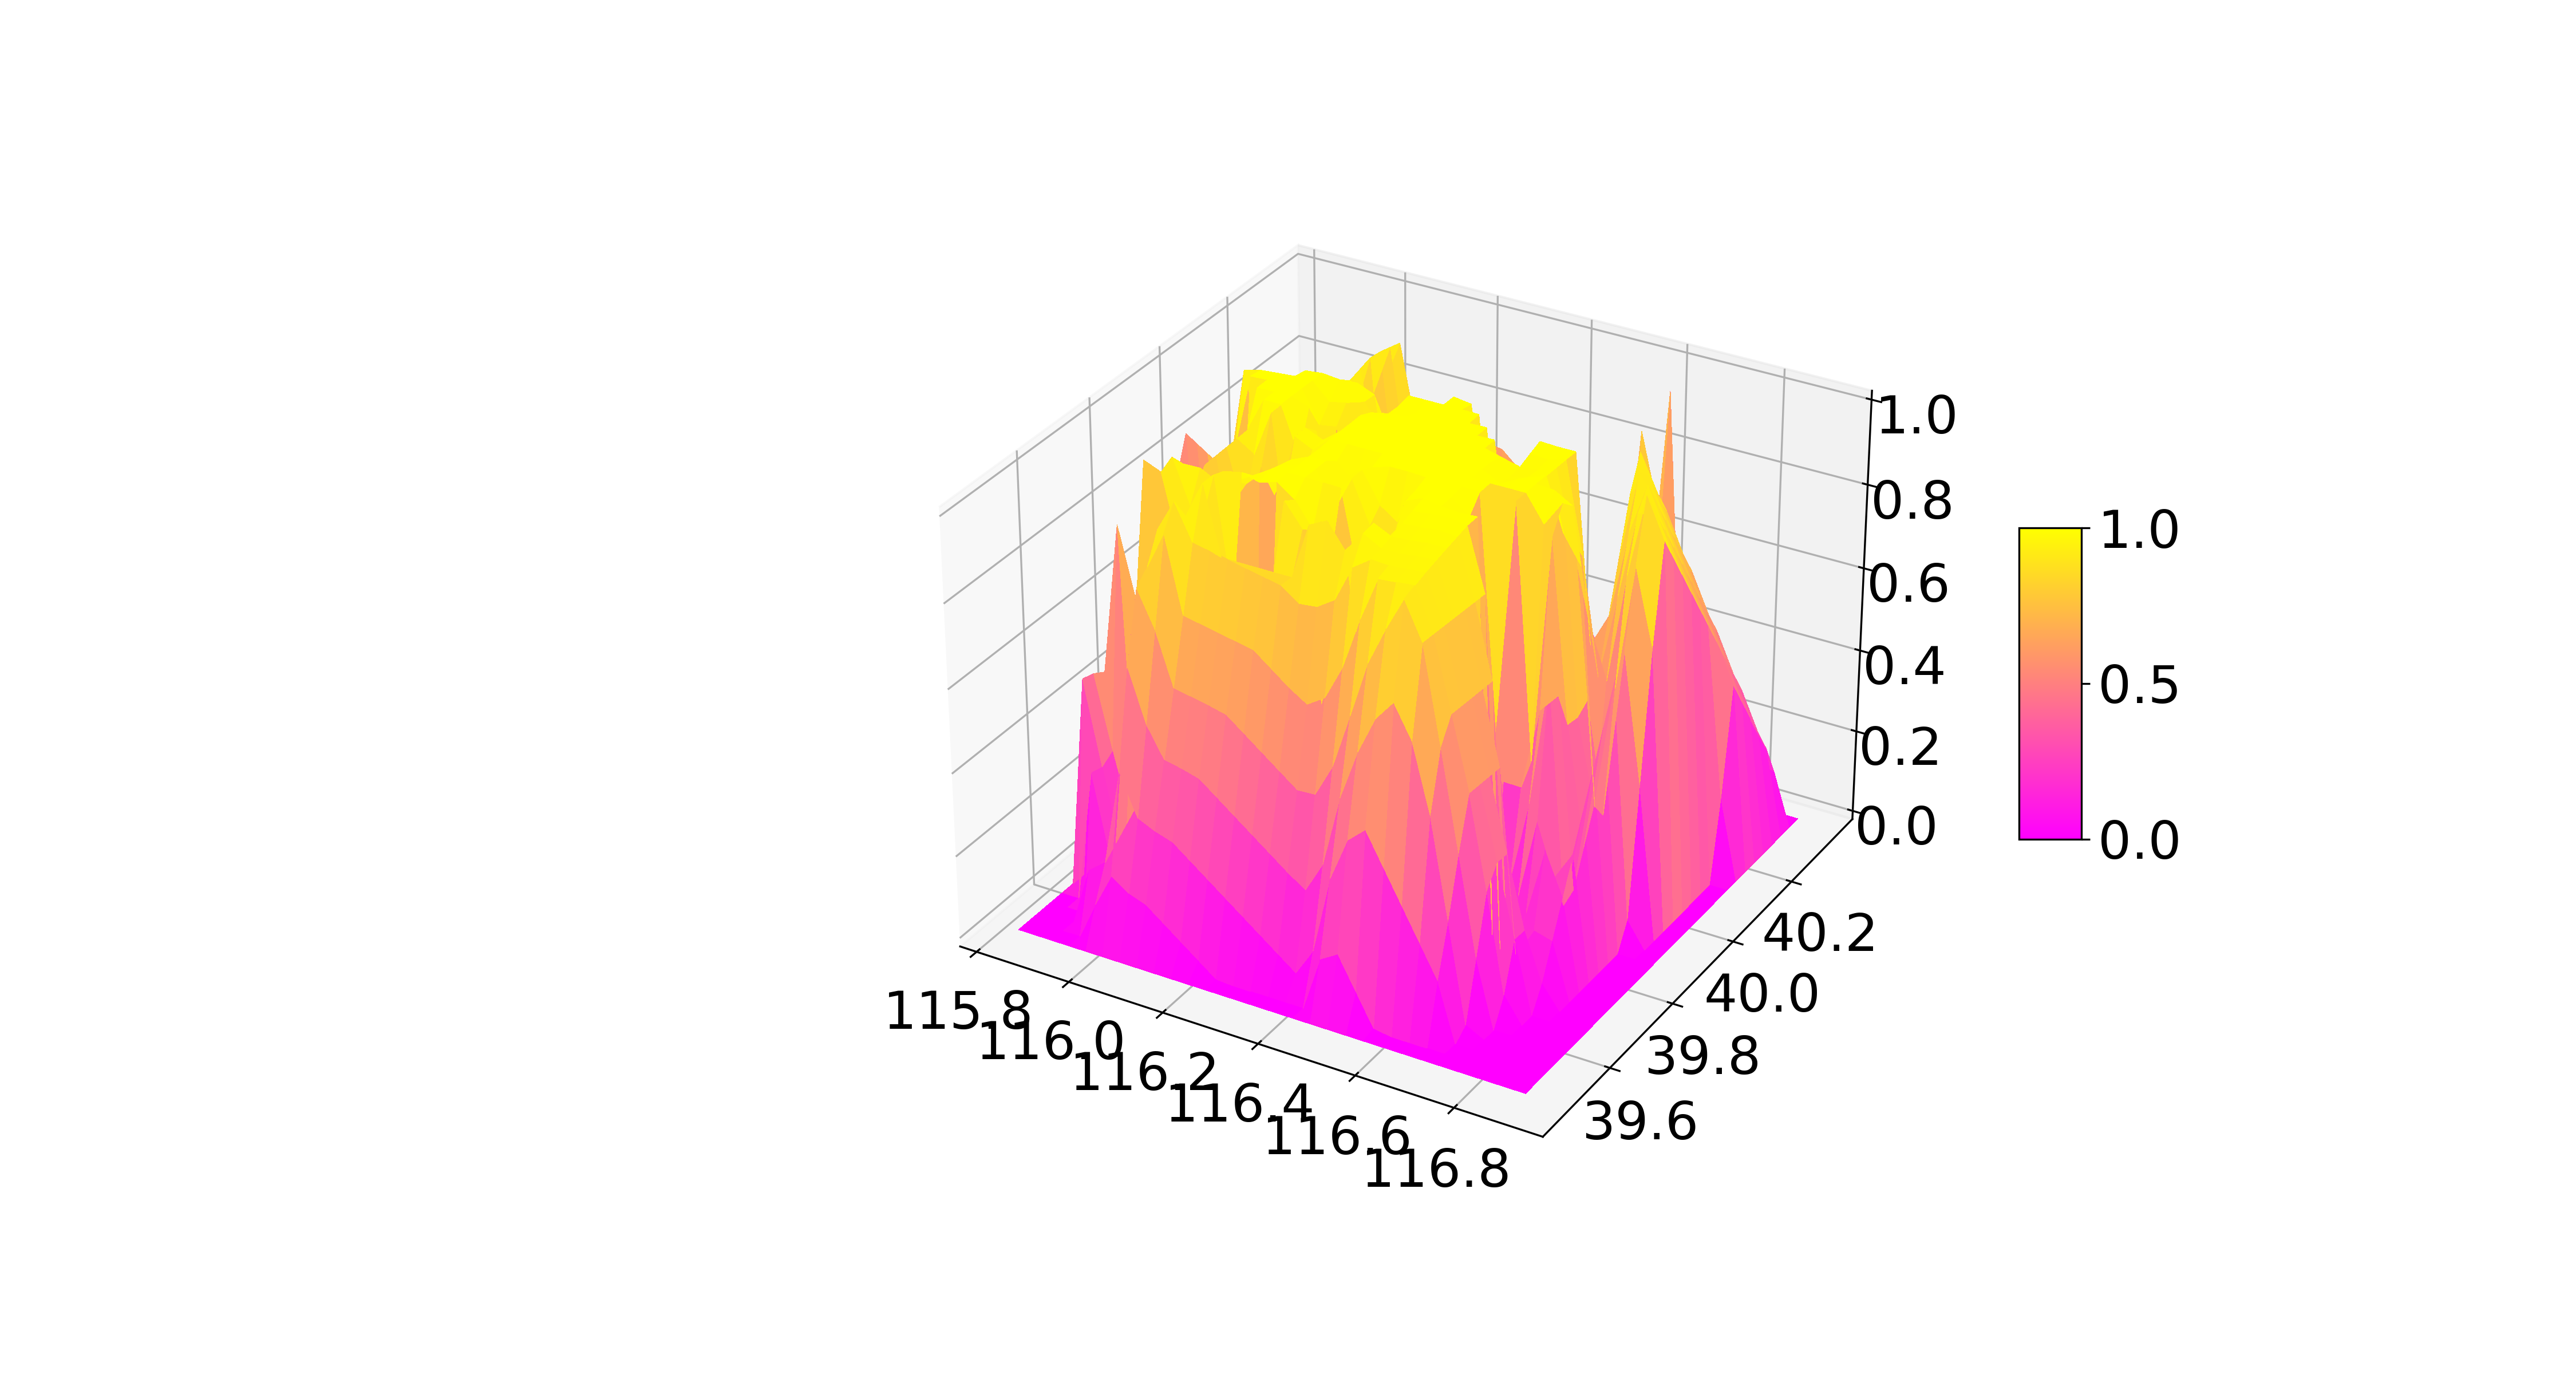
\includegraphics[width=\linewidth]{POIs_coverages_0,00142857_lambda_3D_grid.png}
		\caption{Meshgrid ottenuta per $\lambda = 1/700$}
	\end{subfigure}
	\begin{subfigure}[b]{\linewidth}
		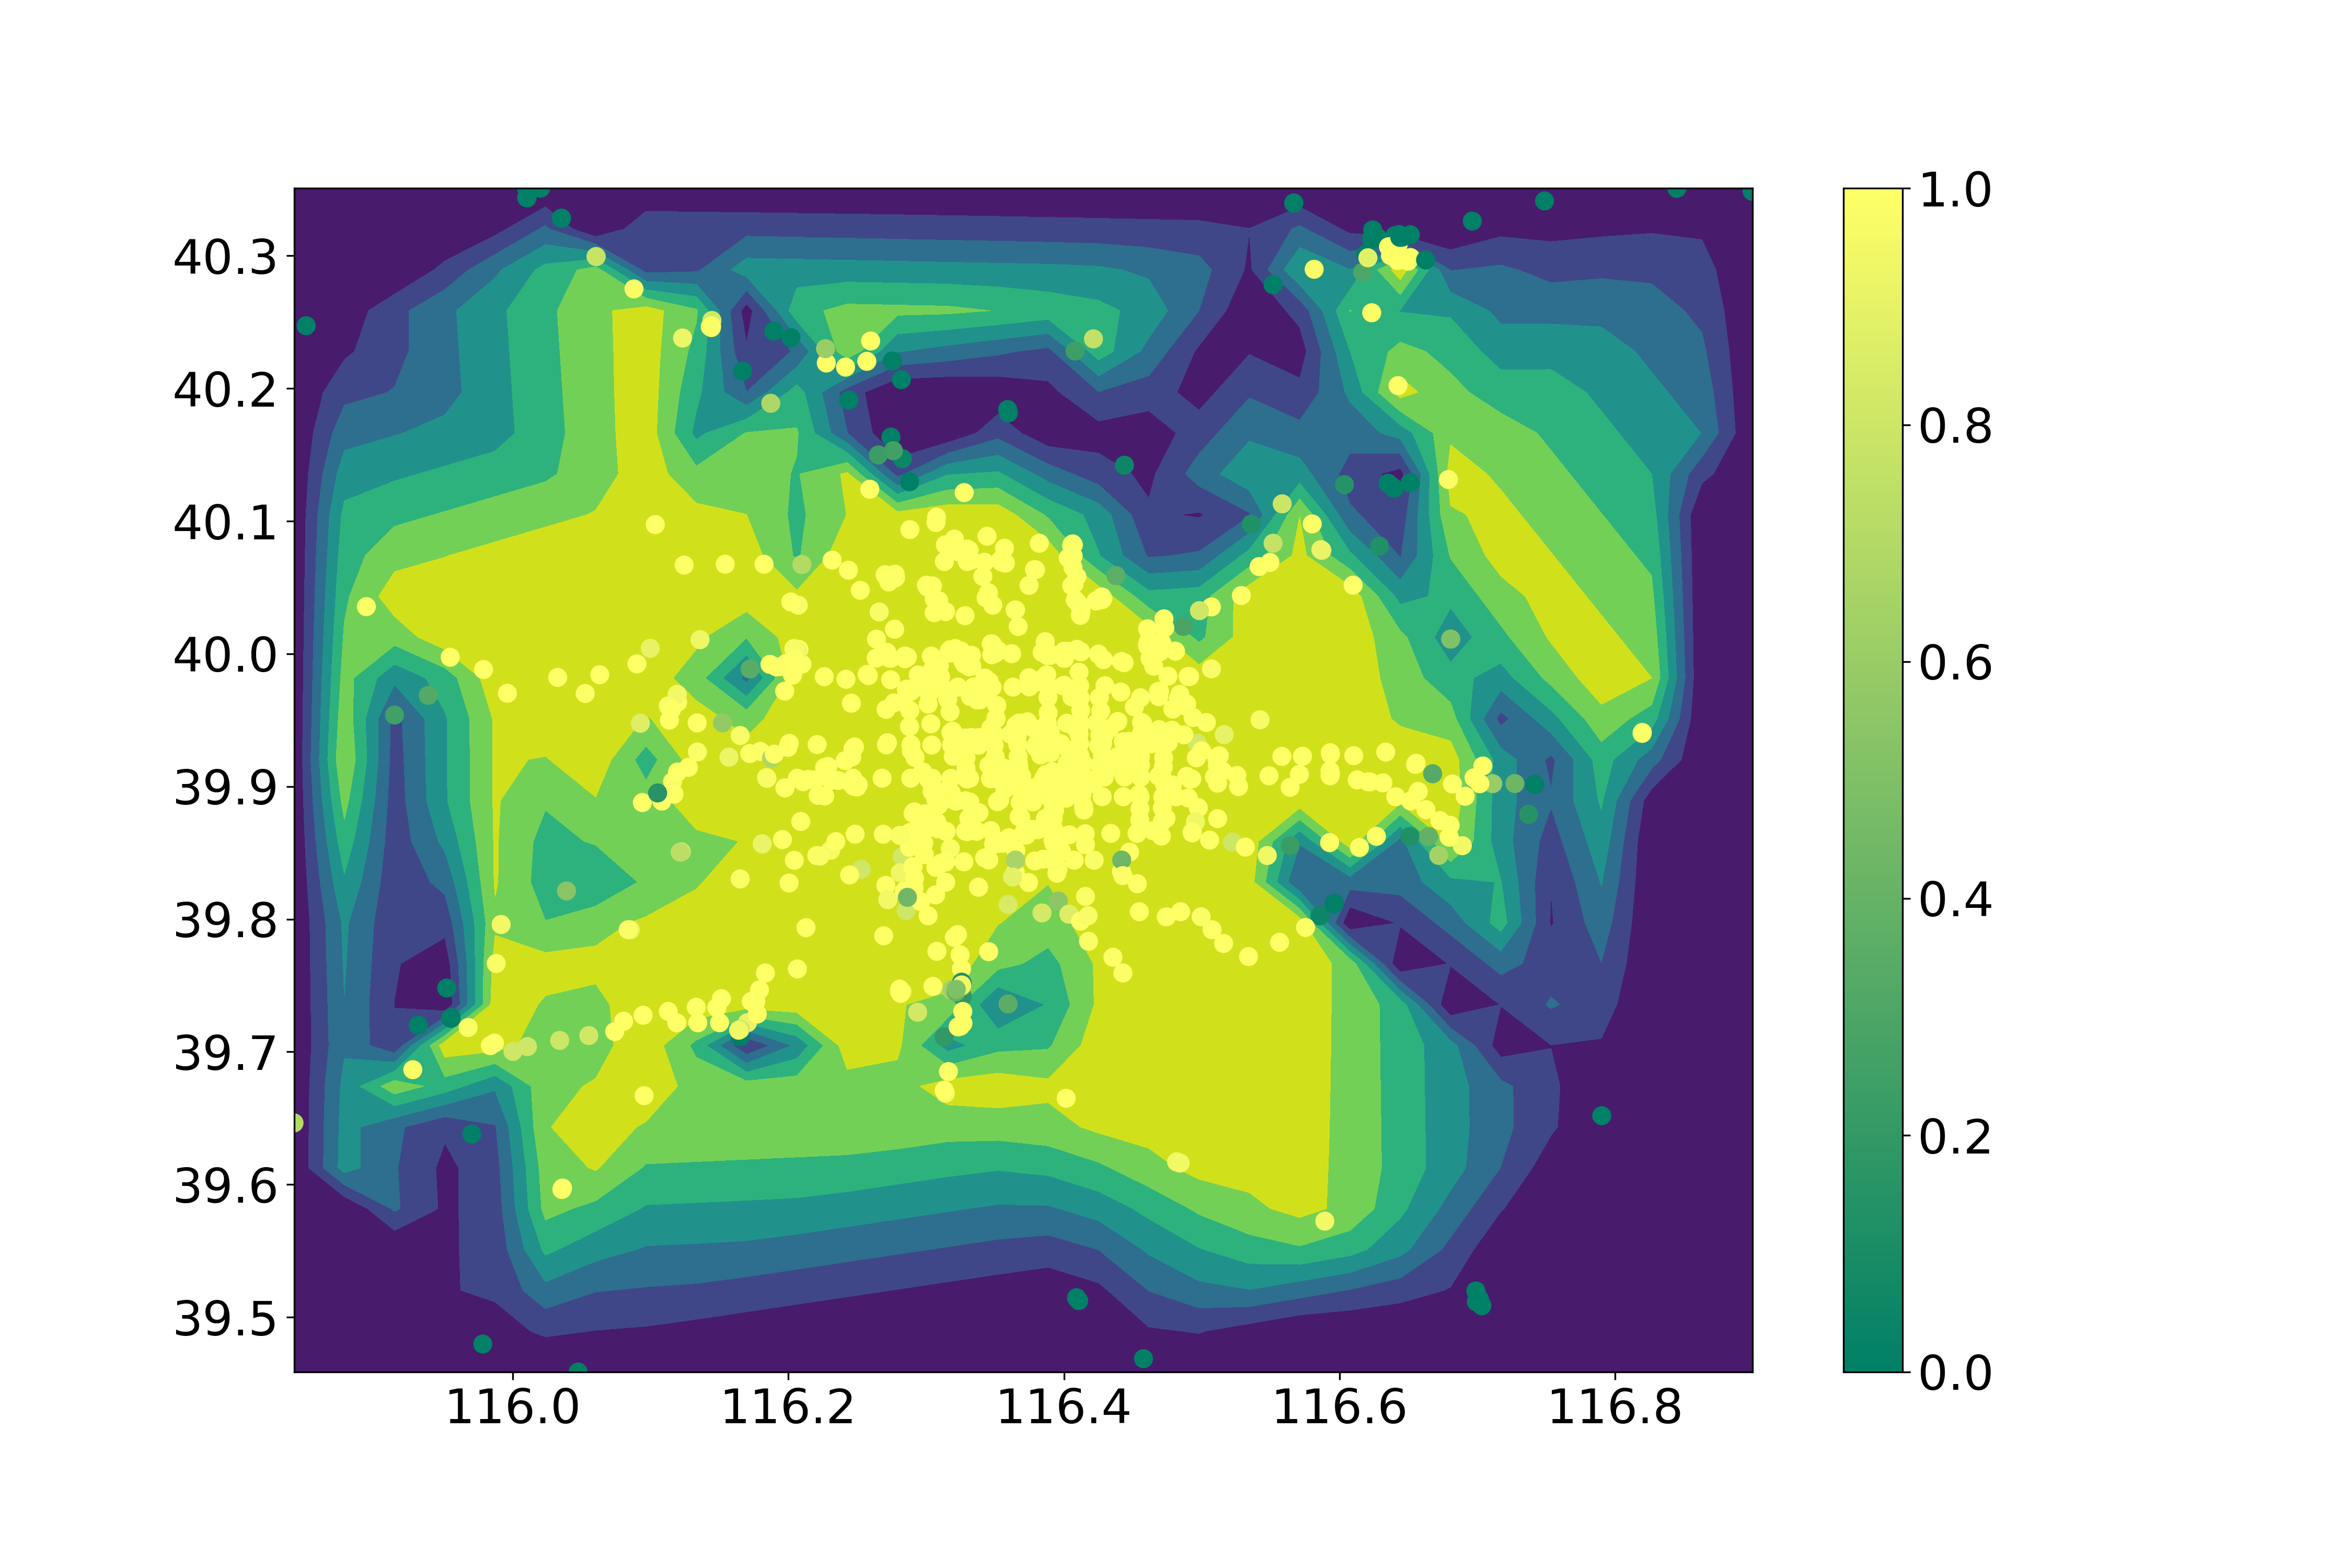
\includegraphics[width=\linewidth]{POIs_coverages_0,00142857_lambda_heatmap.png}
		\caption{Mappa di calore ottenuta per $\lambda = 1/700$}
	\end{subfigure}
	\caption[Risultati POIs, $\lambda = 1/700$]{I risultati ottenuti applicando il modello ai punti di interesse con $\lambda = 1/700$}
	\label{fig:POIs_coverage3}
\end{figure}

\section{Analisi dei risultati ottenuti}

Procediamo adesso con una analisi dei risultati ottenuti per ciascuno scenario e, più in generale, per tutta la sperimentazione.

Le meshgrid e le mappe di calore mostrano la Data Coverage in relazione alle diverse locazioni di raccolta dati. 
La differente scelta delle locazioni ha chiaramente influenzato la mappa di Data Coverage risultante; questo è particolarmente evidente nel caso degli scenari sui flussi di traffico e sui punti di interesse, in cui la relativa sparsità delle locazioni, e la loro assenza nelle zone periferiche della città, porta a dei risultati peculiari.
Ciononostante è bene ricordare che, per i fini specifici del monitoraggio dei flussi di traffico e dei punti di interesse, non siamo interessati a zone con assenza di traffico umano, di conseguenza il risultato ci sembra soddisfacente, ed in linea con le aspettative per ciascuno scenario.
Nelle mappe di calore riguardanti lo scenario di monitoraggio ambientale, si riescono a distinguere bene zone periferiche affatto trafficate, poiché la natura delle locazioni, posizionate a griglia equispaziata, ci permette di valutare con efficacia la Data Coverage in tutta la zona di sensing. Il centro di Pechino ha una Data Coverage praticamente certa e ben distribuita, come si nota dalle figure. 

Fatte queste considerazioni, risulta normale che, ove le locazioni diventino più sparse e distanti dalle traiettorie, la Data Coverage decresca molto rapidamente fino ad arrivare a valori nulli, nelle zone in cui non sono presenti locazioni.
Nei grafici sono evidenti zone con picchi negativi di Data Coverage racchiusi all'interno di aree con una Data Coverage pressoché perfetta.
Questi picchi negativi sono dovuti alla mancanza di traiettorie in quelle specifiche zone, e ci suggeriscono la possibilità di ampliare la strategia di raccolta con piani ad hoc per le suddette zone.

In tutti e tre gli scenari si nota una differenza minima al variare di $\lambda$. Questo è dovuto probabilmente al fatto che le traiettorie, pur aumentate, risultano essere insufficienti a modellare con precisione i pattern di spostamento di persone reali. Per aggiungere realismo alle traiettorie si potrebbero introdurre dei punti di fermata intermedi tra il punto di partenza e quello di arrivo di ciascuna traiettoria sintetica.

Infine, ci sembra opportuno soffermarci brevemente sui limiti del modello.
Poiché $\lambda$ deve modellare il valore di collaboratività degli utenti, è evidente che tale parametro debba essere necessariamente una semplificazione della realtà: con i dati forniti da GeoLife \cite{zheng1, zheng2, zheng3} non possiamo sapere veramente se un utente sarebbe disposto o meno ad accettare una deviazione.
Un altro limite degno di nota è l'aver usato una distribuzione esponenziale nel modello di coverage. Nulla vieta che la probabilità di Data Coverage segua un andamento di tipo diverso, per questo sarebbe interessante provare il modello con altri tipi di distribuzione.
Un'ultima considerazione riguarda le barriere architettoniche e fisiche: nel modello utilizziamo la distanza da una locazione per calcolare la probabilità che un utente sia disposto a raggiungerla e raccogliere i dati, ma  glissiamo sull'esistenza di eventuali barriere architettoniche e fisiche che potrebbero impedire all'utente di raggiungere agilmente la locazione.
Si pensi ad esempio ad una locazione che si trova sulla riva sinistra di un fiume senza ponti: il modello restituirebbe una probabilità di copertura per l'utente che si trova sulla riva destra, tuttavia la raccolta dati sarebbe impossibile, poiché l'utente non avrebbe modo di attraversare il fiume. La Figura \ref{fig:no_coverage_example} mostra questo tipo di problematica.

\begin{figure}
	\centering 
	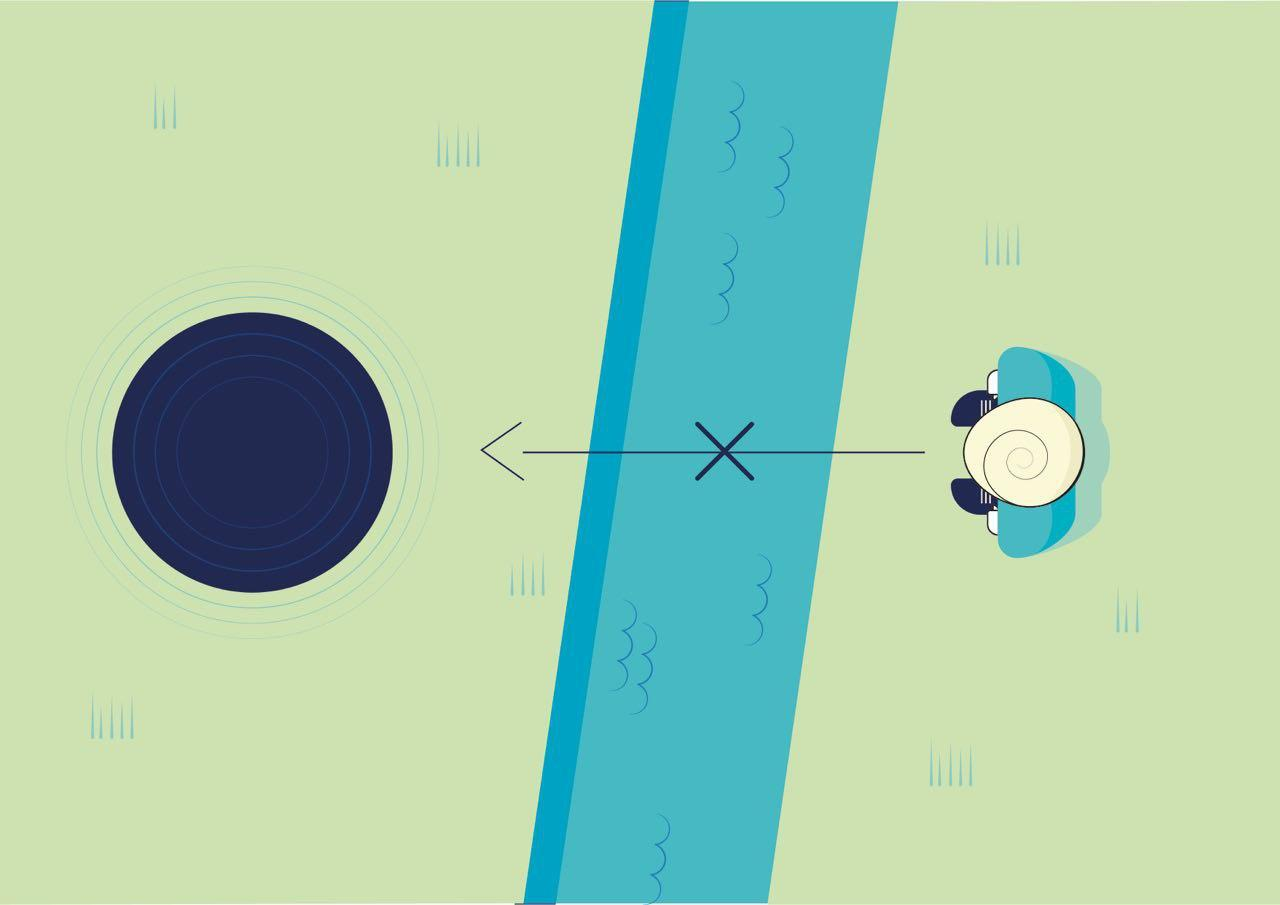
\includegraphics[width=0.7\linewidth]{no_coverage_example.jpg}
	\caption[Esempio di barriera fisica]{Una barriera fisica, in questo caso un corso d'acqua, impedisce all'utente di raggiungere la zona di sensing.}
	\label{fig:no_coverage_example}
\end{figure}

Pur con tutte le semplificazioni citate, i risultati dell'applicazione del modello ci sembrano soddisfacenti, soprattutto in vista di ulteriori sviluppi nella tecnologia del MCS e del miglioramento dei dataset disponibili.
	\chapter{Conclusioni}

Il nostro obiettivo principale è quello di applicare un modello di Data Coverage facilmente replicabile a vari scenari di Mobile Crowdsensing e, contemporaneamente, di sviluppare una strategia efficace per l'arricchimento sintentico dei dataset di mobilità disponibili pubblicamente.
Librerie versatili e complete come scikit-mobility \cite{pappalardo2019scikitmobility} ci hanno aiutato a svolgere compiti affatto banali e a ottenere metriche utili sul nostro dataset. I tool grafici poi, ci hanno permesso di rappresentare risultati di Data Coverage ottenuti grazie al modello descritto nel Capitolo 2 in modo chiaro e diretto.
Grazie a tali librerie, e agli strumenti esplorativi della Data Science, siamo riusciti nel nostro intento di modellare la Data Coverage e di calcolarla sul dataset arricchito, producendo così delle mappe probabilistiche di Coverage che possano essere utilizzate in lavori futuri.
L'implementazione del modello e la sua successiva applicazione a scenari diversi per finalità e composizione è, a nostro avviso, il risultato più interessante di questa tesi.
Ci riteniamo soddisfatti dei risultati che abbiamo raggiunto in questi ambiti, tuttavia ci sono alcuni aspetti del nostro studio che potrebbero essere ampliati e approfonditi in futuro; grazie alla Data Coverage che abbiamo calcolato, infatti, è possibile pianificare uno sviluppo del lavoro che sia guidato da tale metrica.
Vorremmo di seguito descrivere brevemente tre dei possibili sviluppi in questo senso.

\paragraph*{Utilizzo della Data Coverage per il posizionamento di UAV Base Stations}
Grazie alla Data Coverage calcolata, sarà possibile scegliere il posizionamento ottimale per una o più stazioni di ricarica per UAV (unmanned aerial vehicles). Queste stazioni fungeranno da punti di partenza e arrivo per droni a pilotaggio remoto (possibilmente automatico, e schedulato sulla base della evoluzione dinamica della data coverage nella area di sensing) che sorvolino le aree con una Data Coverage pessima o inesistente, al fine di raccogliere loro stessi i dati mancanti.
Tale attività rappresenta la naturale
continuazione di questo lavoro di tesi su cui altri studenti potranno condurre ulteriori attività di ricerca.
Le immagini presenti in Figura \ref{fig:uav_stations} mostrano un possibile posizionamento per le stazioni di ricarica.

\begin{figure}
	\centering
	\begin{subfigure}[b]{\linewidth}
		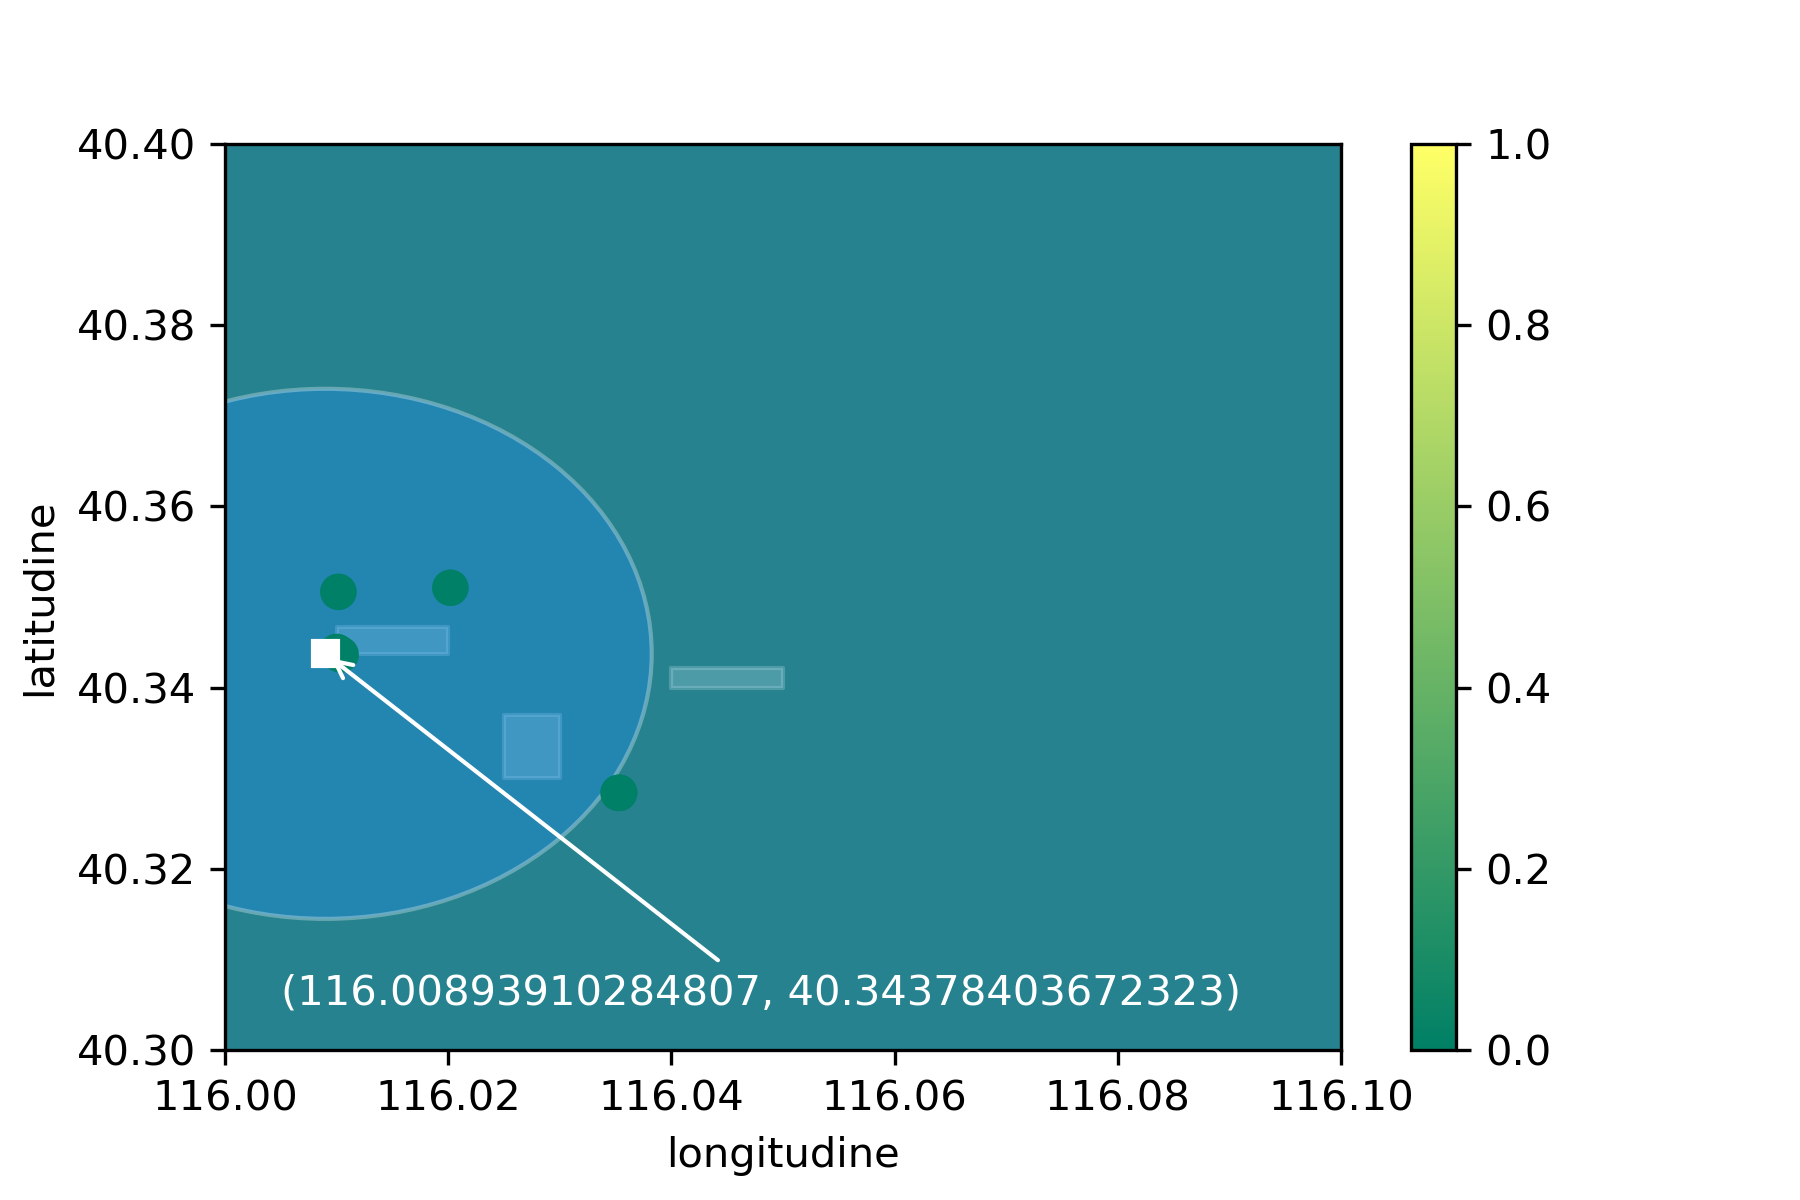
\includegraphics[width=\linewidth]{drone_low_cov_squares.png}
		\caption{Posizionamento su mappa con cattiva Data Coverage. I rettangoli chiari rappresentano zone in cui non è possibile posizionare la stazione di ricarica.}
	\end{subfigure}
	\begin{subfigure}[b]{\linewidth}
		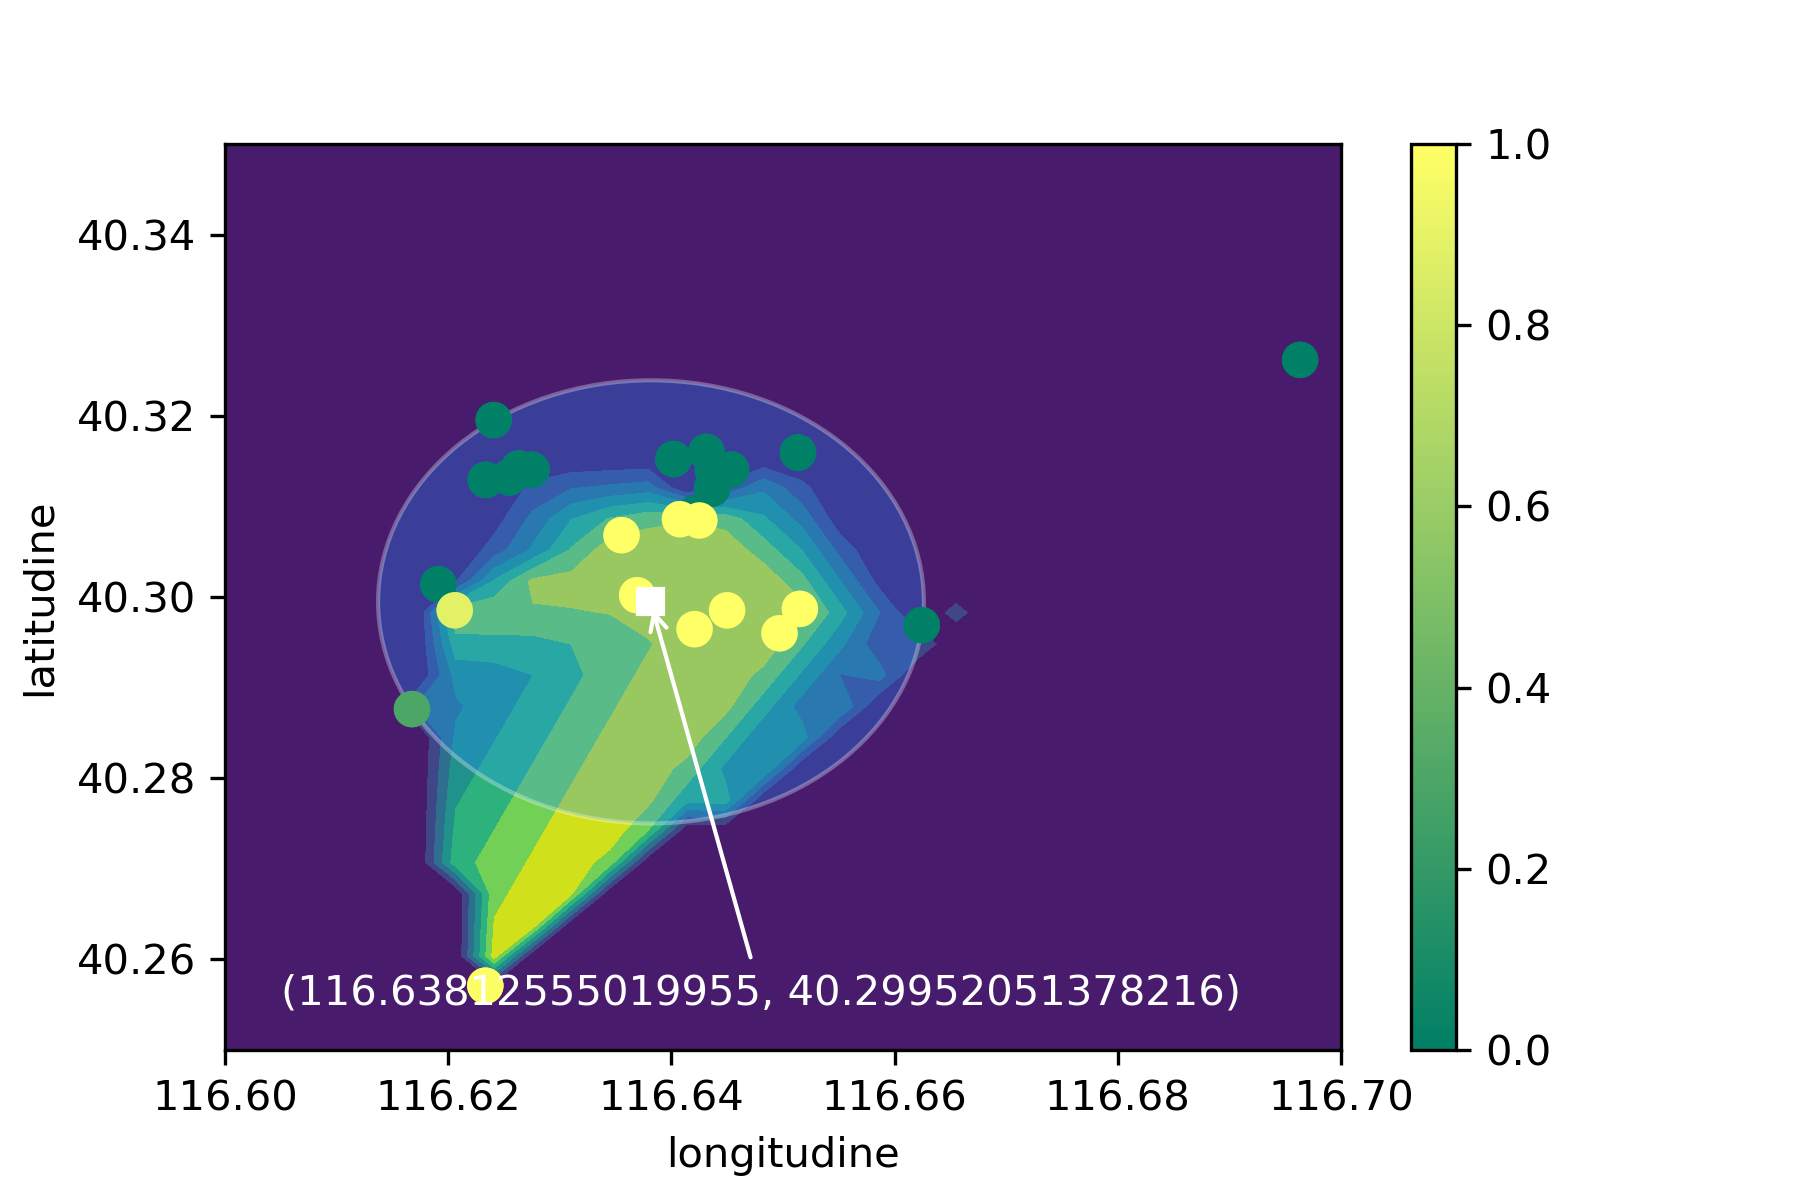
\includegraphics[width=\linewidth]{drone_med_cov.png}
		\caption{Posizionamento su mappa con Data Coverage accettabile.}
	\end{subfigure}
	\caption[Posizionamento di UAV Base Stations]{Esempi di posizionamento di una stazione di ricarica per UAV su una mappa di Data Coverage. I quadrati bianchi rappresentano la posizione della stazione di ricarica, il cerchio attorno ad essi rappresenta il raggio della zona coperta dal drone.}
	\label{fig:uav_stations}
\end{figure}

\paragraph{Calcolo della Coverage a partire dalla mobilità degli utenti tramite strumenti predittivi}
Partendo dalle traiettorie note degli utenti, è possibile sviluppare strumenti predittivi che utilizzino metriche quali la frequenza e la periodicità degli spostamenti dei singoli individui al fine di predirne il posizionamento futuro. Questo permetterebbe lo sviluppo di modelli di Data Coverage predittivi, utili nella pianificazione di campagne di MCS continuative e dinamiche, che sfruttino queste metriche per ottimizzare l'allocazione di risorse umane a materiali in relazione alle necessità future. 

\paragraph{Uso della Data Coverage per ottimizzare la progettazione di architetture di MCS adattive alla mobilità ed alla quantità di dati}
Questo punto si collega strettamente ai due precedenti. La possibilità di predire la Data Coverage futura, assieme alla versatilità dei droni, sono strumenti utili alla progettazione di architetture MCS il più possibile adattive e dinamiche. Nel recente passato, ad esempio, le nostre abitudini giornaliere sono cambiate molto a causa della pandemia di Covid-19 \cite{DiRenzo2020}: le persone tendono a muoversi meno e a evitare assembramenti, riducendo al tempo stesso l'utilizzo di trasporto pubblico. Date queste premesse, è senz'altro interessante teorizzare e sviluppare architetture MCS resilienti a questo tipo di modificazioni strutturali nel comportamento umano.
	\chapter*{Ringraziamenti}

Grazie al Prof. Stefano Chessa per avermi dato fiducia, 
al Dott. Michele Girolami, per la sua pazienza e per avermi insegnato le basi della Data Science,
a Talia che mi sostiene ogni giorno,
ai miei genitori, Andrea e Cristina,
a mio fratello Edoardo,
ai miei zii Stefano e Barbara e al resto della mia famiglia,
a Giacomo per i consigli sempre utili,
a Leonardo per 22 anni di amicizia,
a tutti i miei amici.
	
	\bibliographystyle{ieeetr}
	\bibliography{bibliografia.bib}
	
\end{document}
